\documentclass{article}
\usepackage[utf8]{inputenc}
\usepackage[T2A]{fontenc}
\usepackage[russian]{babel}
\usepackage{amsfonts}
\usepackage{amsmath}
\usepackage{amssymb}
\usepackage{arcs}
\usepackage{fancyhdr}
\usepackage{float}
\usepackage[left=3cm,right=3cm,top=3cm,bottom=3cm]{geometry}
\usepackage{graphicx}
\usepackage{hyperref}
\usepackage{multicol}
\usepackage{stackrel}
\usepackage{xcolor}
\usepackage{epigraph}
\usepackage{tikz}
\usepackage{amsthm}
\usepackage{graphics}
\usepackage{draftwatermark}
\usepackage{ marvosym }
\usepackage{pdfpages}



\def\letus{%
\mathord{\setbox0=\hbox{$\exists$}%
         \hbox{\kern 0.125\wd0%
               \vbox to \ht0{%
                  \hrule width 0.75\wd0%
                  \vfill%
                  \hrule width 0.75\wd0}%
               \vrule height \ht0%
               \kern 0.125\wd0}%
       }%
        }
\def\dbl{\,\,}

\DeclareMathOperator{\sign}{sign}


\newcommand*\lateraleye{%
       \scalebox{0.15}{
    \tikzset{every picture/.style={line width=0.75pt}} 
    \begin{tikzpicture}[x=0.75pt,y=0.75pt,yscale=-1,xscale=1]
    \draw  [line width=1.5]  (300,100.33) .. controls (326,122) and (352,135) .. (378,139.33) .. controls (352,143.67) and (326,156.67) .. (300,178.33) ;
    \draw  [fill={rgb, 255:red, 0; green, 0; blue, 0 }  ,fill opacity=1 ] (308.94,116.33) .. controls (313.87,116.33) and (317.86,125.51) .. (317.85,136.83) .. controls (317.84,148.15) and (313.84,157.33) .. (308.91,157.33) .. controls (303.99,157.32) and (300,148.14) .. (300.01,136.82) .. controls (300.02,125.5) and (304.02,116.32) .. (308.94,116.33) -- cycle ;
    \draw  [draw opacity=0][line width=1.5]  (314.84,166.6) .. controls (311.87,164.64) and (309.14,162.18) .. (306.76,159.24) .. controls (295.12,144.82) and (296.6,124.33) .. (310.07,113.45) .. controls (311.48,112.32) and (312.96,111.33) .. (314.5,110.49) -- (331.14,139.55) -- cycle ; \draw  [line width=1.5]  (314.84,166.6) .. controls (311.87,164.64) and (309.14,162.18) .. (306.76,159.24) .. controls (295.12,144.82) and (296.6,124.33) .. (310.07,113.45) .. controls (311.48,112.32) and (312.96,111.33) .. (314.5,110.49) ;
    \draw  [fill={rgb, 255:red, 255; green, 255; blue, 255 }  ,fill opacity=1 ] (304.43,124.2) .. controls (306.09,124.25) and (307.32,128.01) .. (307.18,132.6) .. controls (307.05,137.19) and (305.59,140.88) .. (303.93,140.83) .. controls (302.27,140.78) and (301.03,137.02) .. (301.17,132.43) .. controls (301.31,127.83) and (302.76,124.15) .. (304.43,124.2) -- cycle ;
    \end{tikzpicture}
    }\,}

\let\vanillaparagraph\paragraph
\let\vanillasubparagraph\subparagraph
\renewcommand{\paragraph}[1]{\vanillaparagraph{#1}\mbox{}\\}
\renewcommand{\subparagraph}[1]{\vanillasubparagraph{#1}\mbox{}\\}

\graphicspath{{../images/}}

\setlength{\parindent}{0pt}

\setcounter{tocdepth}{4}
\setcounter{secnumdepth}{4}

\SetWatermarkText{$\underset{\text{@imodre @snitron}}{\text{ПРОДАМ ГАРАЖ}}$}
\SetWatermarkScale{2}
\SetWatermarkLightness{0.9}

\begin{document}
\DraftwatermarkOptions{stamp=false}
\begin{titlepage}
    \centering
    \vspace*{\baselineskip}
    \rule{\textwidth}{1.6pt}\vspace*{-\baselineskip}\vspace*{2pt}
    \rule{\textwidth}{0.4pt}\\[\baselineskip]
{\LARGE СВЯТОЙ КПК\\ [0.3\baselineskip] \#BlessRNG}\\[0.2\baselineskip]
    \rule{\textwidth}{0.4pt}\vspace*{-\baselineskip}\vspace{3.2pt}
    \rule{\textwidth}{1.6pt}\\[\baselineskip]
    \scshape
    Или как не сдохнуть на 1 семе из-за матана \\
    \vspace*{2\baselineskip}
    Разработали \\[\baselineskip]
    {\Large Тимофей Белоусов\quad @imodre \\ Никита Варламов\quad @snitron \\ Тимофей Цорин \quad @thefattestowl\par}
    \vfill
    v1.3\\
    {\scshape Март 2022-2023} \par
\end{titlepage}

\textbf{Заметки авторов}

В данном конспекте названия всех задач имеют ссылку на своего автора в виде верхнего индекса:
\begin{enumerate}
    \item @imodre
    \item @snitron
    \item @thefattestowl
\end{enumerate}
По любым вопросам и предложениям/улучшениям обращаться в телеграмм к соответвующему автору, или создать Pull Request в \href{https://github.com/snitron/ct-itmo}{Git-репозиторий конспекта (click)}.

\newpage

\begin{flushright}
\emph{Эх\\
Дубинушка\\
Ухнем!}
\end{flushright}

\tableofcontents


\setlength{\parskip}{6pt}%
\newpage
\DraftwatermarkOptions{stamp=true}


\section{Период 1 (Палеозойский)}
\subsection{Важные определения}

\subsubsection{Предел последовательности (\texorpdfstring{$\varepsilon-\delta$}{эпсилон-дельта} определение)\texorpdfstring{$^1$}{}}
\begin{flalign}
\notag
&\letus a \,\text{--- предел последовательности} \, \{x_n\}_{n=1}^\infty&\\
\notag
&\forall \varepsilon > 0 \, \exists N \in \mathbb{N} \, : \, \forall n > N \quad |x_n-a| < \varepsilon&
\end{flalign}
Обозначается $\lim\limits_{n\rightarrow \infty} x_n = a$ ($n\rightarrow\infty$ можно опустить, т.к. а куда ещё ему стремиться в натуральных числах?)

\subsubsection{Метрика, метрическое пространство, подпространство\texorpdfstring{$^1$}{}}
Метрика --- некоторая функция ($\rho: X \times X \rightarrow \mathbb{R}$), определяющая расстояние между элементами в метрическом пространстве. 

Существуют некоторые аксиомы, которым подчиняется метрика:
\begin{enumerate}
    \item $\rho(x, y) = 0 \Leftrightarrow x = y$
    \item $\rho(x, y) = \rho(y, x)$
    \item $\rho(x, z) \le \rho (x, y) + \rho(y, z)$
\end{enumerate}

Метрическое пространство --- пространство, в котором определена метрика (между любыми двумя элементами можно определить расстояние). Обозначается как пара $(X, \rho)$

Подпространство метрического пространства --- метрическое пространство, в котором множество является подмножеством множества исходного пространства, а метрика - сужение исходной метрики на новое множество:
$$
(Y, \rho|_{Y \times Y})\text{, где}\, (X, \rho) \,\text{- исходное пространство, а Y}\, \subset X
$$

\subsubsection{Шар, замкнутый шар, окрестность точки в метрическом пространстве\texorpdfstring{$^1$}{}}
Открытый шар - набор всех точек $x$ в метрическом пространстве $(X, \rho)$, для которых верно $\rho (x, x_0) < r$, где $r$ - радиус шара, $x_0$ - центр шара (Обозн. $B(x_0, r)$).

Замкнутый шар - то же самое, но вместо $<$ стоит $\le$

\subsubsection{Внутренняя точка множества, открытое множество, внутренность\texorpdfstring{$^2$}{}}
\label{ВТМОМВ}
$\left(X, \rho\right)$\textit{ ---  метрическое пространство,} $D \subset X$, $a \in X$

Если $\exists \dbl V_a \subset D \Rightarrow a$ --- \textit{внутренняя точка} множества $D$\\
Если $\forall \, a\in D \dbl a$ --- внутренняя, $\Rightarrow D$ --- \textit{открытое} множество (в $X$)\\
\textit{Внутренностью множества} называется Int $D = \left\{ x \dbl|\dbl x \in D \And x \dbl \text{--- внутренняя}\right\}$\\
Другими словами, \textit{внутренностью D} является:
\begin{enumerate}
    \item объединение всех открытых подмножеств $D$,
    \item максимальное по включению открытое подмножество $D$.
\end{enumerate}

Примечания:
\begin{enumerate}
    \item Int$D$ - открытое множество
    \item Если $D$ открытое $\Leftrightarrow D = $ Int $D$
\end{enumerate}

\subsubsection{Предельная точка множества\texorpdfstring{$^2$}{}}
Если $\forall \dbl r \dbl \dot{V}_a(r) \cap D \ne \varnothing$, то точка $a$ называется \textit{предельной точной множества}

\subsubsection{Замкнутое множество, замыкание, граница\texorpdfstring{$^2$}{}}
Если $D$ содержит все свои \textit{предельные} точки, то такое множество  называется \text{замкнутым}. (Примеры: $X, \varnothing$)

Замыкание $D$ есть: 
\begin{enumerate}
    \item пересечение всех замкнутых множеств, содержащих $D$
    \item минимальное по включению замкнутое множество, содержащее $D$
\end{enumerate}

Граница $D$ - множество граничных точек $D$

\subsubsection{Изолированная точка, граничная точка\texorpdfstring{$^2$}{}}
Если $\exists \dbl r \in \mathbb{R} \dbl : \dbl a \in D \dbl \dot{V_a(r)} \cap D = \varnothing$, то такая точка $a$ называется \textit{изолированной}

Если $\forall \dbl r \in \mathbb{R} \dbl : \dbl a \in D \dbl \dot{V_a(r)}$ сожержит точки как из $D$, так и не из $D$, то такая точка называется \textit{граничной}

\subsubsection{Верхняя, нижняя границы; супремум, инфимум\texorpdfstring{$^2$}{}}

$X \subset \mathbb{R}$

Тогда $\exists M \in \mathbb{R} : \forall x \in X \dbl x \le M$. $M$ --- \textit{верхняя граница}.

$\exists m \in \mathbb{R} : \forall x \in X \dbl x \ge m$. $m$ ---  \textit{нижняя граница}.

\subsubsection{Последовательность, стремящаяся к бесконечности\texorpdfstring{$^1$}{}}
Называется бесконечно большой.
$$
\forall \varepsilon >(<) 0 \, \exists N \,:\, \forall n > N \quad x_n >(<) \varepsilon \Leftrightarrow x_n \rightarrow +\infty(-\infty)
$$
Аналогично, если стремится по модулю, то к беззнаковой бесконечности. 

\newpage
\subsection{Определения}

\subsubsection{Упорядоченная пара\texorpdfstring{$^1$}{}}
Семейство, в котором есть 2 элемента (с учётом порядка)

\subsubsection{Декартово произведение\texorpdfstring{$^1$}{}}
Множество упорядоченных пар. Например $X \times Y$ - все упорядоченные пары, где первый элемент $\in X$, а второй $\in Y$

\subsubsection{Окрестность точки, проколотая окрестность\texorpdfstring{$^1$}{}}
Множество элементов, находящихся на "расстоянии" $< \varepsilon$. Проколотая окрестность \textbf{не} включает сам элемент. В контексте числовой прямой мы можем говорить, что $\{x : |x - x_0| < \varepsilon|\}$ --- проколотая окрестность.

Окрестности обозначаются $V_{x_0}(\varepsilon)$

\subsubsection{Предел последовательности(на языке окрестностей)\texorpdfstring{$^1$}{}}
\begin{flalign}
\notag
&\letus a \text{--- предел последовательности}&\\
\notag
&\forall \varepsilon > 0 \, \exists N\in\mathbb{N} \, : \forall n > N \quad x_n \in V_a(\varepsilon)&
\end{flalign}

\subsubsection{Последовательность\texorpdfstring{$^1$}{}}
Это отображение $D \rightarrow Y$, где $D \in \mathbb{N}$

\subsubsection{Образ и прообраз множества при отображении\texorpdfstring{$^2$}{}}
Отображение - тройка $(X, Y, f)$, где $X, Y$ - множества, а $f$ - некое правило, по которому можно $x \in X$ сопоставить $y \in Y$. Записывается как $f: X \rightarrow Y$

Тогда \textit{образом} множества $A \subset X $ при отображении является множество, такое что:
\begin{equation}
    f(A) = \left\{f(x) \dbl | \dbl x \in A \right\}
\end{equation}

А \textit{прообразом} при $B \subset Y$:
\begin{equation}
    f^{-1}(B) = \left\{x: f(x) \in B \dbl | \dbl x \in X \right\}
\end{equation}

\subsubsection{Инъекция, сюръекция, биекция\texorpdfstring{$^2$}{}}
Если $x_1, x_2 \in X; \dbl x_1 \neq x_2 \Rightarrow f(x_1) \neq f(x_2)$, то такое отображение называется \textit{инъективным (инъекция)}. Другими словами, $f(x) = y$ имеет не более одного решения в $X$

Если $f(X) = Y$, то такое отображение называют \textit{сюръективным (сюръекция)}. Другими словами, $\forall y \in Y \dbl \exists x \in X : f(x) = y$

Если у нас выполняется \textit{инъекция} $+$ \textit{сюръекция}, то такое отображение называют \textit{биективным (биекция)}. Другими словами, для $\forall y \in Y$ найдётся $x \in X$, причём этот $x$ --- единственный.


\subsubsection{Векторнозначная функция, её координатные функции\texorpdfstring{$^1$}{}}
\begin{flushright}
\emph{"У векторнозначной функции векторные значения"}\\
--- Капитан Очевидность
\end{flushright}
\begin{flalign}\notag
&f: X \rightarrow \mathbb{R}^m (\mathbb{C}^m)&
\end{flalign}

Также, можно $f$ записать как $(f_1, f_2, \ldots, f_m)$. $f_i$ и есть координатная функция

\subsubsection{График отображения\texorpdfstring{$^2$}{}}

Пусть дано отображение $(X, Y, f)$. Тогда \textit{графиком} $\Gamma_f$ будет называться множество упорядоченных пар в декартовой системе координат, таких что:

\[\Gamma_f = \left\{(x, y) \in X \times Y : f(x) = y \right\}\]

\subsubsection{Композиция отображений\texorpdfstring{$^2$}{}}

Пусть дано $f: X \rightarrow Y, g: Y \rightarrow Z$. Тогда \textit{композицией} отображений $g \circ f$ будет называться такое отображение $h: X \rightarrow Z$, что:

\[\forall x \in X : h(x) = (g \circ f)(x) = g(f(x))\]

\subsubsection{Сужение и продолжение отображений\texorpdfstring{$^2$}{}}

Пусть задано отображение $f: X \rightarrow Y$. Тогда \textit{сужением}
его на $A \subset X$ будет называться отображение $g = f|_A$, такое что:

\[g: A \rightarrow Y, \forall a \in A : g(x) = f(x)\]

Однако, теперь $f$ для $g$ будет являться \textit{продолжением} ($g$ определена на подмножестве $X$)

\subsubsection{Описание внутренности множества\texorpdfstring{$^2$}{}}
Достаточно подробно определено в\\ \nameref{ВТМОМВ}

\subsubsection{Описание замыкания множества в терминах пересечений\texorpdfstring{$^1$}{}}
$\letus G$ --- произвольное множество.
$$
\overline{G} = \underset{F\supset G, F \text{замк.}}{\bigcap} F
$$
Эквивалент определения "замыкание - пересечение всех замкнутых надмножеств"

\subsubsection{Аксиомы вещественных чисел\texorpdfstring{$^1$}{}}
В $\mathbb{R}$ есть 2 операции:
\begin{enumerate}
    \item Сложение: $+: \mathbb{R} \times \mathbb{R} \rightarrow \mathbb{R}$
    \item Умножение: $\cdot: \mathbb{R} \times \mathbb{R} \rightarrow \mathbb{R}$
\end{enumerate}

\paragraph{Аксиомы поля}
\subparagraph{Аксиомы сложения}
\begin{enumerate}
    \item Ассоциативность: $(a + b + c = a + (b + c)$
    \item Коммутативность: $a + b = b + a$
    \item Нейтральный элемент: $a + 0 = a$
    \item "Обратный элемент": $\exists a' : a + a' = 0$
\end{enumerate}

\subparagraph{Аксиомы умножения}
\begin{enumerate}
    \item Ассоциативность $a(bc) = (ab)c$
    \item Коммутативность $ab = ba$
    \item Нейтральный элемент: $1 \cdot a = a$
    \item Обратный элемент: $\forall a \ne 0 \exists a' : a\cdot a' = 1$
\end{enumerate}

Ещё их объединяет дистрибутивность: $a(b+c) = ab + ac$

\paragraph{Аксиомы порядка}
Когда говорим про порядок, имеем в виду операцию сравнения
\subparagraph{Аксиомы}
\begin{enumerate}
    \item Рефлексивность $a \le a$
    \item Транзитивность $a \le b, b \le c \Rightarrow a \le c$
    \item Антисимметричность $a \ne b \Rightarrow (a \le b) \ne (b \le a)$
    \item Связь сложения и порядка $x \le y \Rightarrow x + z \le y + z$
    \item Связь умножения и порядка $x \ge 0, y \ge 0 \Rightarrow x \cdot y \ge 0$
\end{enumerate}

\subsubsection{Аксиома Кантора, аксиома Архимеда\texorpdfstring{$^1$}{}}
\paragraph{Аксиома Кантора}
$$\letus [a_i, b_i]; [a_{i+1}, b_{i+1}] \subset [a_i, b_i]$$
$$
\bigcap_{i=1}^\infty [a_i, b_i] \ne \varnothing
$$

\paragraph{Аксиома Архимеда}
$$
\forall a, b \in \mathbb{R}, a > 0 \exists n \in \mathbb{N} : a\cdot n > b
$$

\subsubsection{Пополненное множество вещественных чисел, операции и порядок в нем\texorpdfstring{$^2$}{}}

$\overline{\mathbb{R}} = \mathbb{R} \cup \{-\infty, \infty\}$. Казалось бы, а что ещё? Ну, немного есть.

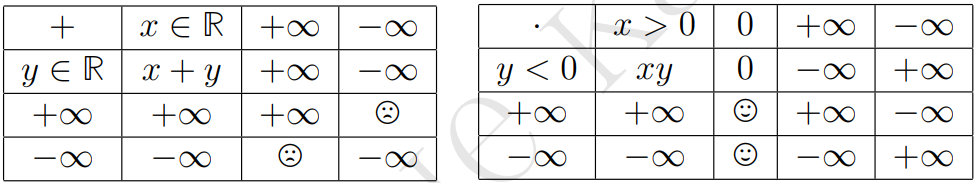
\includegraphics[scale=0.55]{../images/added_R.png}

$\Frowny$ --- операция не определена.

$\Smiley$ --- операция не определена, но в некоторых случаях нам на это пофиг (типа, площадь прямоугольника со сторонами $\infty$ и 0 равна 0)

Неопределённости: $\frac{0}{0}, \frac{\infty}{\infty}, 1^\infty, 0^0, \infty^0, 0 * \infty$

Причём: $-\infty < \infty$ (и ещё можно перечислить операции из таблички)

\subsubsection{Техническое описание супремума\texorpdfstring{$^1$}{}}
$$
b = \sup X = 
\begin{cases}
\exists M \in \mathbb{R} : \forall x \in X \dbl x \le M\\
\forall \varepsilon > 0 \dbl \exists x \in X : M - \varepsilon < x
\end{cases} 
$$

$$
a = \inf X = 
\begin{cases}
\exists m \in \mathbb{R} : \forall x \in X \dbl x \ge m\\
\forall \varepsilon > 0 \dbl \exists x \in X : m - \varepsilon > x
\end{cases} 
$$

\subsubsection{Линейное пространство\texorpdfstring{$^1$}{}}
Также его называют \textit{векторным пространством}. Это пространство, в котором определено множество векторов $X$ и поле $K$.

В этом пространстве определены 2 операции (умножение вектора на число (элемент поля) и сложение векторов):
\begin{enumerate}
    \item $X\times K \rightarrow X$
    \item $X\times X \rightarrow X$
\end{enumerate}

и 7 аксиом:

$\letus x, y, z \in X, \lambda, \gamma \in K$
\begin{enumerate}
    \item $(x + y) + z = x + (y + z)$
    \item $x + y = y + x$
    \item $0 \cdot x = \theta$
    \item $\lambda \cdot (x + y) = \lambda \cdot x + \lambda \cdot y$
    \item $(\lambda + \gamma) \cdot x = \lambda \cdot x + \gamma \cdot x$
    \item $\lambda \cdot (\gamma \cdot x) = (\lambda \cdot x) \cdot \gamma$
    \item $1 \cdot x = x$
\end{enumerate}

\subsubsection{Норма, нормированное пространство\texorpdfstring{$^1$}{}}
Норма - функция, получающая по вектору его "длину". $p: X \rightarrow \mathbb{R}_+$, где $X$ - линейное пространство. Часто обозначают как $||x||$ Имеет 3 свойства:
\begin{enumerate}
    \item $||x|| = 0 \Leftrightarrow x = \theta$
    \item $||\lambda x|| = \lambda ||x||$
    \item $||x + y|| \le ||x|| + ||y||$
\end{enumerate}

Есть ещё полунормы (они не подчиняются 1 свойству). У них есть ещё 4 свойства:
\begin{enumerate}
    \item $p(\sum\limits_{i=1}^n \lambda_i \cdot x_i) \le \sum\limits_{i=1}^n |\lambda_i| \cdot p(x_i)$
    \item $p(\theta) = 0$ (в обратную сторону не работает в отличие от нормы)
    \item $p(-x) = p(x)$
    \item $p(x-y) \ge |p(x) - p(y)|$
\end{enumerate}

Нормированное пространство обозначается парой (X, p)

\subsubsection{Ограниченное множество в метрическом пространстве\texorpdfstring{$^1$}{}}
Ограниченное множество $X$ в метрическом пространстве --- множество, где $\exists x_0 \exists R \quad X \subset B(x_0, R)$

\subsubsection{Скалярное произведение\texorpdfstring{$^1$}{}}
Это отображение $X \times X \rightarrow \mathbb{R}$, где $X$ --- линейное пространство. Обозначается $(x, y).\, x, y \in X$ Существует 3 свойства, определяющие скалярное произведение:
\begin{enumerate}
    \item $(x, y) = (y, x)$
    \item $(\lambda \cdot x + \gamma \cdot y, z) = \lambda \cdot (x, z) + \gamma \cdot (y, z)$
    \item $(x, x) = 0 \Leftrightarrow x = \theta$, иначе $>0$
\end{enumerate}

Свойства скалярного произведения:
\begin{enumerate}
    \item $(x, y + z) = (x, y) + (x, z)$
    \item $(\lambda \cdot x, y) = \lambda \cdot (x, y)$
    \item $(\theta, y) = (x, \theta) = 0$
    \item $|(x, y)|^2 \le (x, x)(y, y)$ (\nameref{КБШ})
    \item $\sqrt{(x, x)}$ - норма, порождённая скалярным произведением.
\end{enumerate}

\newpage
\subsection{Важные теоремы}

\subsubsection{Теорема о двух городовых\texorpdfstring{$^1$}{}}
\textbf{Формулировка:}

$x_n \rightarrow a, z_n \rightarrow c, y_n \rightarrow b, x_n \le y_n \le z_n, a = c \Rightarrow b = a$

\textbf{Доказательство:}

По теореме о предельном переходе в неравенствах для последовательностей, $a \le b \le c$. 

Допустим $b \ne a$. Тогда $\exists N : \forall n > N \quad |x_n - a| \le \frac{|a - b|}{2} \And |y_n - b| \le \frac{|a - b|}{2} \And |z_n - a| \le \frac{|a - b|}{2} \Rightarrow$ $z_n$ и $y_n$ не пересекаются. Но поскольку $z_n \ge y_n$, а $a < b$, у нас противоречие.

\subsubsection{Теорема Кантора о стягивающихся отрезках\texorpdfstring{$^2$}{}}

\textbf{Формулировка}

Пусть дана система вложенных отрезков $[a_1, b_1] \supset [a_2, b_2] \supset \ldots$

И при этом $(b_n - a_n) \rightarrow_{n \rightarrow \infty} 0$

Тогда $\exists ! c \in \bigcap_{n = 1}^\infty{[a_n, b_n]}$ и при этом $a_n \rightarrow c$ и $b_n \rightarrow c$

\textbf{Доказательство}

$\rhd$ Для $\forall n \in \mathbb{N} \dbl a_n \le c \le b_n$. Вычтем из обоих сторон $a_n : 0 \le c - a_n \le b_n - a_n$. Слева 0, справа б.м. последовательность, следовательно $c - a_n \rightarrow_{n \rightarrow \infty} \Rightarrow a_n \rightarrow c$. Для $b_n$ аналогично.

Единственность $c$ можно доказать:
\begin{enumerate}
    \item по теореме о единственности предела
    \item Пусть $c, d \in \bigcap_{n = 1}^\infty{[a_n, b_n]}$. Тогда $\forall n \in \mathbb{N} : a_n \le c \le b_n$ и $a_n \le d \le b_n$. Вычтем их друг из друга, получим $a_n - b_n \le c - d \le b_n - a_n$. Предельно переходим и получаем $0 \le c - d \le 0 \Rightarrow c = d$
\end{enumerate}
$\lhd$


\subsubsection{Теорема об арифметических свойствах предела последовательности в нормированном пространстве и в \texorpdfstring{$\mathbb{R}$}{R}\texorpdfstring{$^1$}{}}

\textbf{Формулировка:}

$(X, p)$ - нормированное пространство\\
$\letus x_n \rightarrow x_0, y_n \rightarrow y_0.\, x, y, x_0, y_0 \in X$\\
$\{\lambda\in \mathbb{R}\}_{n=1}^\infty, \lambda_n \rightarrow \lambda_0$
\begin{enumerate}
    \item $x_n + y_n \rightarrow x_0 + y_0$
    \item $x_n - y_n \rightarrow x_0 - y_0$
    \item $\lambda_n \cdot x_n \rightarrow \lambda_0 \cdot x_0$
    \item $||x_n|| \rightarrow ||x_0||$
    \item Для $\mathbb{R}$: $\frac{x_n}{y_n} \rightarrow \frac{x_0}{y_0}$
\end{enumerate}

\textbf{Доказательство:}

\begin{enumerate}

\item \begin{flalign}
\notag &\exists N_1 \in \mathbb{N} : \forall n > N_1 \quad ||x_n - x_0|| < \frac{\varepsilon}{2}&\\
\notag &\exists N_2 \in \mathbb{N} : \forall n > N_2 \quad ||y_n - y_0|| < \frac{\varepsilon}{2}&\\
\notag &N := \max(N_1, N_2)&\\
\notag &||x_n + y_n - (x_0 + y_0)|| = &\\
\notag &=||(x_n - x_0) + (y_n - y_0)|| \underset{\text{н-во треугольника}}{\le} ||(x_n - x_0)|| + ||(y_n - y_0)|| \le \frac{\varepsilon}{2} + \frac{\varepsilon}{2} = \varepsilon&
\end{flalign}

\item Банально, сведём к первому+третьему $||x_n - y_n|| = ||x_m + (-1)y_n|| \rightarrow x_0 + (-1)y_n = x_0 - y_n$

\item $||\lambda_n x_n - \lambda_0 x_0|| = ||\lambda_n x_n + \lambda_n x_0 - \lambda_n x_0 - \lambda_0 x_0|| = ||\underset{\text{огр.}}{\lambda_n} \underset{\text{б.м.}}{(x_n - x_0)} + \underset{\text{огр.}}{x_0} \underset{\text{б.м.}}{(\lambda_n - \lambda_0)}|| \rightarrow 0$

\item $| ||x_n|| - ||x_0|| | \underset{\text{Треугольник для полунорм}}{\le} ||\underset{\text{б.м.}}{x_n - x_0}|| \rightarrow 0$

\item 
\begin{flalign}
\notag &\frac{x_n}{y_n} = x_n\frac{1}{y_n} \rightarrow x_0\frac{1}{y_0} = \frac{x_0}{y_0}&\\
\notag &\text{Но это не работает, т.к. мы не знаем куда стремится} \frac{1}{y_n}&\\
\notag &y_n \,\text{огр., т.к.} \,y_0 \ne 0\,\text{, а}\, y_n \,\text{сходящаяся (по т. об ограниченности сх. посл.)}&\\
\notag &\left|\frac{1}{y_n} - \frac{1}{y_0}\right| = \left|\frac{y_0-y_n}{y_n y_0}\right| = \left|\underset{\text{огр.}}{\frac{1}{y_n}}\underset{\text{огр.}}{\frac{1}{y_0}}\underset{\text{б.м.}}{\frac{y_0-y_n}{1}}\right|\rightarrow 0&
\end{flalign}

\end{enumerate}


\subsubsection{Теорема об арифметических свойствах предела последовательности (в \texorpdfstring{$\overline{\mathbb{R}}$}{R с чертой}).\texorpdfstring{\\}{} Неопределённости\texorpdfstring{$^1$}{}}
\textit{Теорема об арифметических свойствах предела последовательности (в $\overline{\mathbb{R}}$)}

\textbf{Формулировка}

$a, b \in \overline{\mathbb{R}}, x_n \rightarrow a, y_n \rightarrow b$
\begin{enumerate}
    \item $x_n \pm y_n \rightarrow a\pm b$
    \item $x_n \cdot y_n \rightarrow a\cdot b$
    \item $\frac{x_n}{y_n} \rightarrow \frac{a}{b}$ (Разумеется, $y_n, b \ne 0$)
\end{enumerate}
Это работает только когда пределы не создают неопределённости. Они как раз представлены дальше

\textbf{Доказательство}
$\rhd$
Положим $x_n \rightarrow +\infty, y_n \rightarrow b$
\begin{enumerate}
    \item $\forall \varepsilon > 0 \exists N : \forall n > N \quad x_n > \varepsilon - b \Rightarrow x_n + y_n > \varepsilon$ (работает т.к. $y_n$ огр. снизу)
    \item $\forall \varepsilon > 0 \exists N : \forall n > N \quad x_n > \frac{\varepsilon}{b} \Rightarrow x_n \cdot y_n > \varepsilon$ (работает т.к. $b \ne 0$)
    \item $\forall \varepsilon > 0 \exists N : \forall n > N \quad x_n > \varepsilon \cdot b \Rightarrow \frac{x_n}{y_n} > \varepsilon$
\end{enumerate}
$\lhd$

\textit{Неопределённости}

Я не понимаю, что тут это делает. Вроде как определение, без доказательств, но записано как теорема...
\begin{enumerate}
    \item $\infty + -\infty$
    \item $\pm \infty \cdot 0$
    \item $\frac{\pm \infty}{\pm \infty}$
    \item $\frac{0}{0}$
\end{enumerate}


\newpage
\subsection{Теоремы}

\subsubsection{Законы де Моргана\texorpdfstring{$^2$}{}}
\textbf{Напоминалка}
\begin{align}
\bigcup_{\alpha \in A}{X_\alpha} &= \left\{ x : \exists \alpha \in A \,\, x \in X_a\right\}\\
\bigcap_{\alpha \in A}{X_\alpha} &= \left\{ x : \forall \alpha \in A \,\, x \in X_a\right\} 
\end{align}

\textbf{Формулировка:}
\begin{equation*}
    \left\{X_\alpha\right\}_{\alpha \in A}\textit{ - семейство множеств, }Y\textit{ - множество. Тогда: }
\end{equation*}
\begin{align}
Y \setminus \bigcup_{\alpha \in A}{X_\alpha} &= \bigcap_{\alpha \in A}{\left(Y \setminus X_\alpha\right)}\\
Y \setminus \bigcap_{\alpha \in A}{X_\alpha} &= \bigcup_{\alpha \in A}{\left(Y \setminus X_\alpha\right)}\\
Y \cap \bigcup_{\alpha \in A}{X_\alpha} &= \bigcup_{\alpha \in A}{\left(Y \cap X_\alpha\right)}\\
Y \cup \bigcap_{\alpha \in A}{X_\alpha} &= \bigcap_{\alpha \in A}{\left(Y \cup X_\alpha\right)}
\end{align}

\textbf{Доказательство:}
\begin{enumerate}
    \item $\rhd$ Рассмотрим закон (1). Обозначим левую часть за $\mathbb{L}$, а правую за $\mathbb{R}$. Тогда $x \in \mathbb{L}$
    означает, что $x \in Y$ и $x \notin \cup_{\alpha \in A} X_\alpha$. По определению \textbf{объединения}, это значит, что $x \in Y$ и $x \notin X_\alpha$ для $\forall \alpha \in A$. Вуаля, по опрeделению \textbf{пересечения} получается, что $x \in \mathbb{R}$. $\lhd$ \\ (2) доказывается аналогично.
    \item $\rhd$ Рассмотрим закон (3). Обозначим левую часть за $\mathbb{L}$, а правую за $\mathbb{R}$. Тогда $x \in \mathbb{L}$
    означает, что $x \in Y$ и $\exists \alpha_0 \in A \,\,:\,\, x \in X_{\alpha_0}$. Иными словами: $\exists \alpha_0 \in A \,\,:\,\, x \in Y \cap X_{\alpha_0}$. Воу, получилось определение \textbf{объединения} для $\mathbb{R}$. $\lhd$ \\ (4) доказывается аналогично.
\end{enumerate}

\subsubsection{Единственность предела и ограниченность сходящейся последовательности\texorpdfstring{$^1$}{}}
\paragraph{Единственность предела:}

\subparagraph{Формулировка:}
$\letus a$ и $b$ --- пределы последовательности $x_n$ $\Rightarrow a = b$

\subparagraph{Доказательство:}

Положим, $a \ne b$ 
\begin{flalign}
\notag &\varepsilon := |a - b| / 2&\\
\notag &\exists N_1 : \forall n > N_1 \quad |x_n - a| < \varepsilon&\\
\notag &\exists N_2 : \forall n > N_2 \quad |x_n - b| < \varepsilon&\\
\notag &N:= \max(N_1, N_2) + 1&\\
\notag &|x_N - a| < \varepsilon \And |x_N - b| < \varepsilon \,\text{, что невозможно, т.к.}\, V_a(\varepsilon) \,\text{и}\, V_b(\varepsilon) \, \text{не пересекаются.}&
\end{flalign}

\paragraph{Ограниченность сходящейся последовательности}

\subparagraph{Формулировка:}
Сходящаяся последовательность ограничена.

\subparagraph{Доказательство:}
Тривиально. Возьмём предел ($a$) последовательности. Возьмём любой $\varepsilon$. 
Для него мы можем узнать $N$, для которого все элементы находятся ближе данного $\varepsilon$. 
Далее возьмём $\max\limits_{i=1}^N|x_i - a|$. 
Это и будет радиусом шара, в котором находятся все элементы последовательности


\subsubsection{Теорема о предельном переходе в неравенствах для последовательностей и для функций\texorpdfstring{$^1$}{}}
\textbf{Формулировка:}

$x_n < y_n, \, x_n \rightarrow a, y_n \rightarrow b \Rightarrow a \le b$

\textbf{Доказательство:}
\begin{flalign}
\notag &\varepsilon := |a - b| / 2&\\
\notag &\exists N_1 : \forall n > N_1 \quad |x_n - a| < \varepsilon&\\
\notag &\exists N_2 : \forall n > N_2 \quad |y_n - b| < \varepsilon&\\
\notag &N:= \max(N_1, N_2)&\\
\notag &\forall n > N \quad |x_n - a| < \varepsilon \And |y_n - b| < \varepsilon, \, \text{а поскольку эти 2 окрестности не пересекаются и}&\\ 
\notag &x_n < y_n\,\text{, то}\, a < b&
\end{flalign}
Для функций аналогично


\subsubsection{Бесконечно малая последовательность\texorpdfstring{$^1$}{}}
\textbf{Формулировка:}

Произведение бесконечно малой последовательности на ограниченную равно бесконечно малой последовательности.

\textbf{Доказательство:}
\begin{flalign}
\notag &\letus x_n \rightarrow 0, \sup |y_n| = K&\\
\notag &\forall \varepsilon > 0 \, \exists N \in \mathbb{N} : \forall n > N \quad |x_n| < \frac{\varepsilon}{\max(K, 1)} \Rightarrow |x_n \cdot y_n| < \varepsilon&
\end{flalign}


\subsubsection{Открытость открытого шара\texorpdfstring{$^2$}{}}
\textbf{Формулировка:}

Открытый шар --- открыт.

\textbf{Доказательство:}

$B(a, r) = \left\{ x \in X : \rho(a, x) < r\right\}$ \textsc{BASED.}

$\rhd$

Пусть $b \in B(a, r)$. Тогда $B(b, r - \rho(a, b)) \subset B(a, r)$ (это надо доказать).

Докажем! Пусть $x \in B(b, r - \rho(a, b))$. Тогда (по определению открытого шара) $\rho(x, b) < r - \rho(a, b)$

$\rho(x, a) \le \rho(x, b) + \rho(b, a) < r$ \textit{ВЖУХ, и неравенство треугольника!}

Следовательно, $\rho(x, a) < r \Rightarrow x \in B(a, r) \Rightarrow B(b, r - \rho(a, b)) \subset B(a, r)$

Следовательно, для любой (произвольной) точки $b$ существует такая окрестность (шар), что $B(b, r - \rho(a, b)) \subset B(a, r) \Rightarrow b$ --- внутренняя.
Тогда все точки внутри открытого шара --- внутренние, и, следовательно, по определению он --- открытое множество.
$\lhd$

\subsubsection{Теорема о свойствах открытых множеств\texorpdfstring{$^2$}{}}

\textbf{Формулировка}
\begin{align}
    \bigcup_{\alpha \in A} &G_\alpha \textit{--- открытое множество}\\
    \bigcap_{k = 1}^{n} &G_k \textit{--- открытое множество}
\end{align}

\textbf{Доказательство}

(9) $\rhd$ Возьмём $\alpha \in A; \dbl x \in G_\alpha$. Так как $G_\alpha$ --- открытое, следовательно, $\exists B(x, r) \subset G_\alpha$. А раз он содержится в одном множестве, логично, что он уже тем более содержится в их объединении. $\lhd$

(10) $\rhd$ Возьмём $x \in \bigcap_{k = 1}^{n} G_k $. Так как этот $x$ содержится в каждом из множеств $G_k$, существует $n$ шаров $B(x, r_k)$, причём каждый шар является подмножеством $G_k$. Давайте введём $r = \min_{k = 1}^n{r_k}$. Тогда шар $B(x, r)$ точно содержится в каждом $G_k$, а, следовательно, и в их пересечении. $\lhd$

\textit{Примечание:}

Пересечение бесконечного количества открытых множеств не обязательно открыто! Пример:

$$
\bigcap_{n=1}^\infty{\left(-\frac{1}{n},\frac{1}{n}\right)} = \left\{0\right\}
$$

\subsubsection{Теорема о связи открытых и замкнутых множеств\texorpdfstring{\\}{} Свойства замкнутых множеств\texorpdfstring{$^2$}{}}

\paragraph{Теорема о связи открытых и замкнутых множеств}
\textbf{Формулировка}

$G$ --- открыто $\Leftrightarrow$ $G^c$ --- замкнуто

\textbf{Доказательство}

\textit{Всё это верно в силу случайности выбираемых точек!}

$\fbox[\Leftarrow] \rhd$ Возьмём $x \in G$. Т.к. $G^c$ --- замкнуто, а $x \notin G^c$, следовательно, $x$ не является предельной точкой для $G^c$ (значит, что $\exists r \in \mathbb{R} : \dot{V_x(r)} \cap G = \varnothing$). Причём окрестность можно взять и не выколотую, т.к.  $x \notin G^c$. Тогда, $V_x \cap G^c = \varnothing$. Но по определению дополнения это значит, что $V_x \subset G$! Следовательно, $x$ --- внутренняя точка для $G \Rightarrow$ оно открытое. $\lhd$

$\fbox[\Rightarrow] \rhd$ Возьмём $x$ --- предельную точку для $G^c$. То есть, любая $\dot{V_x} \cap G^c \neq \varnothing$. Следовательно, $x$ не является внутренней для $G$ (потому что внутренняя точка входит в множество с какой-то окрестностью полностью, а таких окрестностей нету). Следовательно, $x \notin G$, т.к. оно открыто и содержит только внутренние точки. А раз точка не принадлежит множеству, то точно принадлежит его дополнению. $\lhd$

\paragraph{Свойства замкнутых множеств}
\textbf{Формулировка}

$G_a$ --- \textit{замкнутые}

\begin{align}
    \bigcap_{\alpha \in A}&{G_a} \textit{--- замкнуто}\\
    \bigcup_{k=1}^{n}&{G_a} \textit{--- замкнуто}
\end{align}

\textbf{Доказательство}

Вуаля, применяем законы де Моргана и предыдущую теорему:
\begin{equation*}
X \setminus \bigcup_{\alpha \in A}{G_\alpha^c} = \bigcap_{\alpha \in A}{X \setminus G_\alpha^c} = \bigcap_{\alpha \in A}{G_\alpha}
\end{equation*} 

\begin{equation*}
X \setminus \bigcap_{k=1}^{n}{G_\alpha^c} = \bigcup_{k=1}^{n}{X \setminus G_\alpha^c} = \bigcup_{k=1}^{n}{G_\alpha}
\end{equation*} 

\textit{Примечание:}

Объединение бесконечного числа замкнутых множеств не обязательно замкнуто! Пример:

\begin{equation*}
\bigcup_{q \in \mathbb{Q}}{\left\{q\right\}} = \mathbb{Q} \text{ не замкнуто в } \mathbb{R}
\end{equation*} 

\subsubsection{Аксиома Архимеда. Плотность множества рациональных чисел в \texorpdfstring{$\mathbb R$}{R}\texorpdfstring{$^2$}{}}

\paragraph{Свойства замкнутых множеств}
\textbf{Формулировка}

\begin{equation*}
    \forall x > 0, y > 0 \in \mathbb{R} \dbl \exists n \in \mathbb{N} : nx > y
\end{equation*}

(следовательно, существуют сколь угодно большие натуральные числа)

\textbf{Доказательство (аксиомы, лол) ПОКА НЕ ЗНАЮ, КАК-ТО ЧЕРЕЗ СУПРЕМУМ}

\paragraph{Плотность множества рациональных чисел в \texorpdfstring{$\mathbb R$}{R}}
\textbf{Формулировка}

Множество $A \subset X$ всюду плотно в $X$, если $\forall x, y, x < y (x, y) \cap A \neq \varnothing$

$\mathbb{Q}$ всюду плотно в $\mathbb{R}$

\textbf{Доказательство}

$\rhd$ Пусть $x, y \in \mathbb{R}, x < y$. Тогда $\frac{1}{y - x} > 0$ и (по аксиоме Архимеда) $\exists n \in \mathbb{N} : n > \frac{1}{y - x} \Rightarrow \frac{1}{n} < y - x$. Пусть $c = \frac{[nx] + 1}{n} 
\left(c \in \mathbb{Q}\right)$

\[c \le \frac{nx + 1}{n} = x + \frac{1}{n} < x + y - x < y \]
\[c > \frac{nx + 1 - 1}{n} = x\]

Следовательно $c \in (x, y)$ $\lhd$

\subsubsection{Неравенство Бернулли\texorpdfstring{$^2$}{}}

\textbf{Формулировка}

$\forall x \in \mathbb{R} > -1  \dbl n \in \mathbb{N} \dbl (1 + x)^n \ge 1 + nx$

\textbf{Доказательство}

$\rhd$ По индукции!

База (\textsc{BASED}):

$n = 1 \Rightarrow 1 + x \ge 1 + x$

Предположение: $(1 + x)^n \ge 1 + nx$

Переход:
\[(1 + x)^{(n + 1)} = (1 + x)(1 + x)^n \ge (1 + x)(1 + nx) = 1 + nx + x + nx^2 = 1 + (n + 1)x + nx^2 \ge 1 + (n + 1)x\]$\lhd$

\subsubsection{Теорема о существовании супремума\texorpdfstring{$^2$}{}}

\textbf{Формулировка}

\textit{Примечание: тут докажем про ограниченное сверху (супремум) множество, для инфимума аналогично}

Всякое непустое ограниченное сверху подмножество $X \subset \mathbb{R}$ имеет верхнюю грань.

\textbf{Доказательство}

$\rhd$
Так как множество ограничено сверху, то $\exists M \in \mathbb{R} : x \in X \dbl x \le M$. Супер. Возьмём $x_0 \in X$ и создадим отрезок $[x_0, M] = [a_1, b_1]$ ($x_0 \le M$ по определению верхней грани). Заметим, что этот отрезок удовлетворяет двум свойствам:

$$
\text{1) } [a_1, b_1] \cap X \neq \varnothing \quad \text{ и } \quad \text{2) } (b_1, +\infty) \cap X = \varnothing
$$

Шикарно. Теперь выберем точку $d_i = \frac{a_{i-1} + b_{i-1}}{2}$. Если справа нету элементов множества $X$, то смещаем $b_i$ в $d_i$. Если справа элементы есть, то смещаем $a_i$ в $d_i$. Таким образом, мы бинпоиском подбираемся всё ближе и ближе к супремуму (двигаем отрезочек вправа). Причём все наши отрезки --- вложенные! И свойства 1) и 2) так же выполняются. 

ACHTUNG! Наши отрезки ещё и стягиваются! И действительно, ведь $\frac{b_i - a_i}{2^{n - 1}}$ стремится к 0. Следовательно, по теореме Кантора о стягивающихся отрезках, существует всего одна точка $c$, к которой стремятся $a_n$ и $b_n$.

Проверим, что $c\text{ -- }\sup X$. По построению $\forall x \in X : x \le b_n \underset{\text{по теореме о предельном переходе в неравенствах}}{\Rightarrow} x \le c$. Значит, $c$ -- верхняя граница.

Теперь докажем, что для $\forall \varepsilon > 0 \dbl \exists x \in X : c - \varepsilon < x$. Так как $a_n \rightarrow c$, то $c - a_n < \varepsilon \Rightarrow c - \varepsilon < a_n$. То есть, с некоторого натурального $n$ все члены последовательности будут больше $c - \varepsilon$ при заданном $\varepsilon$. А так как выполнялось свойство 1), то найдётся $x \in [a_n, b_n] \subset X$.
$\lhd$

\subsubsection{Лемма(ы) о свойствах супремума\texorpdfstring{$^2$}{}}

\textbf{Формулировка}

\begin{align}
    D \subset E \subset X &\Rightarrow \sup D \le \sup E\\
    \forall \lambda \in \mathbb{R} > 0&: \sup{\lambda D} = \lambda \sup D\\
    \sup {-D} &= -\inf{D}
\end{align}

\textbf{Доказательство}

(13) $\rhd$ Заметим, что $\sup E$ является верхней гранью для $D$ (т.к. $D \supset E$). Следовательно, $\sup D \le \sup E$ $\lhd$

(14) $\rhd$ Для всякого $x \in D$ верно, что $x \le \sup D$. Домножим на $\lambda \Rightarrow \lambda x \le \sup \lambda D \Rightarrow \sup{\lambda D} = \lambda \sup{D}$ $\lhd$

(15) $\rhd \sup -D : \forall x \in -D \dbl x \le \sup{-D}$. Домножим на $(-1) \Rightarrow -x \ge -\sup{-D}$. Тогда $-\sup{-D}$ является нижней границей для $D \Rightarrow -\sup{-D}=\inf{D} \Rightarrow \sup{-D}=-\inf{D} \dbl \lhd$

\subsubsection{Теорема о пределе монотонной последовательности\texorpdfstring{\\}{}(Вейерштрасс in da house)\texorpdfstring{$^2$}{}}

\textbf{Формулировка}

Если последовательность $x_n$ монотонна и ограничена сверху (снизу --- аналогично), то она имеет конечный предел

\textbf{Доказательство}
$\rhd$
Поскольку $x_n$ ограничена, то $\exists M = \sup E$, причём $\forall \varepsilon > 0 \exists x_n : M - \varepsilon < x_n$.

Так как она ещё и монотонна, что $\forall n \in \mathbb{N} \exists N \in \mathbb{N} : x_N \ge x_n$. Mix it!

\[\forall \varepsilon > 0 :  M - \varepsilon < x_n \le x_N \le M < M + \varepsilon\]

Получается, что в $\varepsilon$-окрестности точки $M$ лежит бесконечно большое количество элементов $\{x_n\} \Rightarrow M$ --- предел последовательности.
$\lhd$

\subsubsection{Определение числа e, соответствующий замечательный предел\texorpdfstring{$^2$}{}}

\textbf{Формулировка}

$x_n = \left(1 + \frac{1}{n}\right)^n$ сходится

\textbf{Доказательство}

Заведём $y_n = \left(1 + \frac{1}{n}\right)^{(n + 1)}$. Очевидно, что эта последовательность ограничена снизу единичкой.

Но это ещё не всё! Она ещё и убывающая. Докажем!

\[\frac{y_{n-1}}{y_n} = \frac{\left(\frac{n}{n-1}\right)^n}{\left(\frac{n+1}{n}\right)^{n+1}} = \left(\frac{\frac{n}{n-1}}{\frac{n+1}{n}}\right)^{n+1}\frac{1}{\frac{n}{n-1}} = \left(\frac{n^2}{n^2 - 1}\right)^{n + 1}\frac{n - 1}{n} = \left(1 + \frac{1}{n^2 - 1}\right)^{n + 1}\frac{n - 1}{n}\]

\[\ge_{\text{по неравенству Бернулли}} \left(1 + \frac{n + 1}{n^2 - 1}\right)\frac{n - 1}{n} = 1\]

Ура, монотонна + ограничена $\Rightarrow$ имеет предел. А по теореме об арифметических свойствах предела $x_n = \frac{y_n}{1 + \frac{1}{n}}$ и $x_n$ имеет предел.

\[\lim{\left(1 + \frac{1}{n}\right)^n} = e\]

\subsubsection{Неравенство Коши-Буняковского в линейном пространстве, норма, порождённая скалярным произведением\texorpdfstring{$^1$}{}}
\label{КБШ}
\paragraph{Неравенство Коши-Буняковского}

\textbf{Формулировка:}

$|(a, b)|^2 \le (a, a) \cdot (b, b). a, b \in X$ (линейное пространство).

\textbf{Доказательство:}
\begin{flalign}
\notag &(a + \lambda b, a + \lambda b) = \lambda(a, b) + (a, a) + \lambda(b, a) + \lambda^2 (b, b) = 
(a, a) + 2\lambda(a, b) + \lambda^2(b, b)&\\
\notag &\letus \lambda = -\frac{(a, b)}{(b, b)}&\\
\notag &(a, a) - \frac{2(a,b)^2}{(b, b)} + \frac{(a, b)^2}{(b, b)} =
(a, a) - \frac{(a, b)^2}{(b, b)}=\frac{(a, a)(b, b) - (a, b)^2}{(b, b)}&
\end{flalign}
Т.к. $(a + \lambda b, a + \lambda b) \ge 0$ и знаменатель $(b, b) \ge 0$, то и числитель ($(a, a)(b, b) - (a, b)^2 \ge 0$) $\Rightarrow (a, a)(b, b) \ge (a, b)^2$

\paragraph{Норма, порождённая скалярным произведением}

\textbf{Формулировка:}

$p(a) = \sqrt{(a, a)}$ --- норма.

\textbf{Доказательство:}
\begin{enumerate}
    \item $||a|| = 0 \Leftrightarrow a = \theta$. Очевидно из свойств скалярного произведения.
    \item $||\lambda a|| = |\lambda| ||a||$. Так же очевидно.
    \item $||a + b|| \le ||a|| + ||b||$. $||a + b|| = \sqrt{(a + b, a + b)}.||a + b||^2 = (a + b, a + b) = (a, a) + (a, b) + (b, a) + (b, b) \le(a, a) + \sqrt{(a, a)}\sqrt{(b, b)} + \sqrt{(a, a)}\sqrt{(b, b)} + (b, b) = (a, a) + 2\sqrt{(a, a)}\sqrt{(b, b)} + (b, b)$. $(||a|| + ||b||)^2 = (a, a) + 2\sqrt{(a, a)}\sqrt{(b, b)} + (b, b)$
\end{enumerate}


\subsubsection{Леммы о непрерывности скалярного произведения и покоординатной сходимости в \texorpdfstring{$\mathbb{R}^n$}{n-мерном R}\texorpdfstring{$^1$}{}}
\paragraph{Непрерывность скалярного произведения}

\textbf{Формулировка:}

$X$ - линейное пространство со скалярным произведением. $\exists$ норма, порождённая скалярным произведением.
\begin{flalign}
\notag &x_n \rightarrow x_0&\\
\notag &y_n \rightarrow y_0&\\
\notag &(x_n, y_n) \rightarrow (x_0, y_0)&
\end{flalign}

\textbf{Доказательство:}
\begin{flalign}
\notag &|(x_n, y_n) - (x_0, y_0)| = |(x_n, y_n) - (x_0, y_n) + (x_0, y_n) - (x_0, y_0)| \le&\\
\notag&\le|(x_n, y_n) - (x_0, y_n)| + |(x_0, y_n) - (x_0, y_0)| = |(x_n-x_0, y_n)| + |(x_0, y_n-y_0)| \underset{\text{КБШ}}{\le}&\\ \notag&\le\underset{\text{б.м.}}{||x_n-x_0||}\cdot\underset{\text{огр.}}{||y_n||} + \underset{\text{огр.}}{||x_0||} \cdot \underset{\text{б.м.}}{||y_n-y_0||}\rightarrow 0&
\end{flalign}


\paragraph{Покоординатная сходимость в \texorpdfstring{$\mathbb{R}^n$}{n-мерном R}}

\textbf{Формулировка:}

$x^{(n)}_k$, где $(n)$ - индекс последовательности, $k \in \{1, 2, \ldots, m\}$ - номер координаты в $\mathbb{R}^m$. Метрика Евклидова.

$x^{(n)} \rightarrow a \Leftrightarrow \forall k \quad x^{(n)}_k \rightarrow a_k$

\textbf{Доказательство:}

Common:
$$
\forall k |x_k-a_k| \underset{\text{1 слагаемое}}{\le} \sqrt{\sum_{k=1}^m(x_k - a_k)^2} \le \sqrt{m} \max_{k=1}^m(x_k - a_k)
$$

$\Rightarrow$

$$
\forall k |x_k-a_k| \underset{\text{1 слагаемое}}{\le} \sqrt{\sum_{k=1}^m(x_k - a_k)^2} \underset{\text{метрика}}{\rightarrow} 0 \Rightarrow \forall k x_k \rightarrow a_k
$$

$\Leftarrow$

$$
\sqrt{\sum_{k=1}^m(x_k - a_k)^2} \le \sqrt{m} \max_{k=1}^m|x_k - a_k| \underset{\text{все слагаемые} \rightarrow 0}{\rightarrow} 0
$$




\newpage



\section{Период 2 (Мезозойский)}
\subsection{Важные определения}
\subsubsection{Определения предела отображения (3 шт)\texorpdfstring{$^2$}{}}

\begin{enumerate}
    \item По Коши на $\varepsilon - \delta$ языке:
    \[\forall \varepsilon > 0 \dbl \exists \delta > 0 : \forall x \in D \setminus \{a\} : \rho_X(a, x) < \delta : \rho_Y(f(a), A) < \varepsilon\]
    \item По Коши на языке окрестностей:
    \[\forall V_A \exists \dot{V_a} :
     F(V_a \cap D) \subset V_A\]
     \item По Гейне на языке последовательностей:
     \[\forall \{x_n\}, x_n \in D \setminus \{a\}, x_n \rightarrow a : f(\{x_n\}) \rightarrow A\]
\end{enumerate}

TL;DR отсюда следует и определение предела \textit{функции}: Пусть $f: D \subset \mathbb{R} \rightarrow \mathbb{R}, a \in \mathbb{R}$ --- предельная точка $D$, $A \in \mathbb{R}$.

Тогда $A$ --- предел функции $f$ в точке $a$.


\subsubsection{Компактное множество\texorpdfstring{$^2$}{}}

Если множество $K \subset \bigcup_{\alpha \in A}G_\alpha$, то  семейство множеств $\left\{G_\alpha\right\}_{\alpha \in A}$ называется \textit{покрытием} множества $K$. Если при этом все множества $G_\alpha$ ещё и открытые, то такое покрытие называют открытым.

Подмножество $K$ метрического пространства $X$ называется \textit{компактным}, если из любого открытого покрытия можно извлечь конечное подпокрытие.

\[\forall \left\{G_\alpha\right\}_{\alpha \in A} : K \subset \bigcup_{\alpha \in A}G_\alpha, G_\alpha \textit{ --- открытые в } X, \quad \exists \alpha_1, \alpha_2 \ldots \alpha_n : K \subset \bigcup_{k = 1}^nG_{\alpha_k}\]


\subsubsection{Непрерывное отображение (4 определения)\texorpdfstring{$^1$}{}}
$f : D \subset X \rightarrow Y$
\begin{enumerate}
    \item Дешёвое: существует конечный предел в точке $x_0$ и равен образу в этой точке (работает только для предельных точек)
    \item $\varepsilon-\delta$: $\forall \varepsilon > 0 \exists \delta > 0 : \forall x \in D \setminus \{x_0\}: \rho_X(x, x_0) < \delta \quad \rho_Y(f(x), f(x_0)) < \varepsilon$
    \item Окрестности: $\forall V_{f(x_0)} \exists \dot{V}_{x_0} : \forall x \in \dot{V}_{x_0} \quad f(x) \subset V_{f(x_0)}$
    \item Последовательности: $\forall \{x_n \in D\setminus\{x_0\}\} \rightarrow x_0 \quad f(x_n) \rightarrow f(x_0)$
\end{enumerate}

\subsubsection{о маленькое\texorpdfstring{$^2$}{}}

Пусть $X$ --- метрическое пространство, $f: D \subset X \rightarrow \mathbb{R} (\mathbb{C}). a$ --- предельная точка $D$, и тогда если $\exists \dbl \varphi: D \rightarrow \mathbb{R} (\mathbb{C}) : f(x) = \varphi(x)g(x)$, причём $\exists V_a$ такая что $\varphi(V_a \cap D)$ --- бесконечно малая при всех допустимых $x$, то тогда говорят что $f(x)$ бесконечно малая по сравнению с $g(x)$ при $x \rightarrow a$.

\subsubsection{Эквивалентные функции, таблица эквивалентных\texorpdfstring{$^2$}{}}

Пусть $X$ --- метрическое пространство, $f: D \subset X \rightarrow \mathbb{R} (\mathbb{C}). a$ --- предельная точка $D$, и тогда если $\exists \dbl \varphi: D \rightarrow \mathbb{R} (\mathbb{C}),  : f(x) = \varphi(x)g(x)$, --- при всех $x \in V_a \cap D$, то тогда говорят что $f(x)$ эквивалентна по сравнению с $g(x)$ при $x \rightarrow a$. ($\varphi(x) \rightarrow 1$)

\[\sin x \approx \arcsin x \approx \tan x \approx \arctan x \approx e^x - 1 \approx x\] при $\varphi \rightarrow 1$.


\subsubsection{Функция, дифференцируемая в точке\texorpdfstring{$^1$}{}}
\label{ФункДифТоч}
Пусть $f: \langle a, b \rangle \rightarrow \mathbb{R}, x_0 \in \langle a, b \rangle$

Есть 2 определения:
\begin{enumerate}
\item 
Если $\exists \lim\limits_{\Delta x \rightarrow 0} \frac{f(x + \Delta x) - f(x)}{\Delta x} = k \in \mathbb{R}$, то $f$ дифференцируема в $x_0$, а $k$ --- производная в точке $x_0$

\item
Если $\exists A \in \mathbb{R} : f(x) = f(x_0) + A(x - x_0) + o(x - x_0)$, то $f$ дифференцируема в $x_0$, а $A$ --- производная в точке $x_0$. 
$o(x - x_0)$ означает, что при приближении $x$ к $x_0$ погрешность формулы $\rightarrow 0$
\end{enumerate}

\subsubsection{Производная\texorpdfstring{$^1$}{}}
Имхо, всё уже определено в \nameref{ФункДифТоч}

\newpage
\subsection{Определения}

\subsubsection{Топологическое пространство, топология\texorpdfstring{$^2$}{}}

$X$ --- множество, тогда \textit{топологическим пространством} называется пара множество --- система его подмножеств $(X, W)$, если выполнены следующий условия ($W \subset 2^X$):

\begin{enumerate}
    \item \[\varnothing, X \in W\]
    \item \[\forall \{G_k\}_{k = 1}^n \bigcap_{k = 1}^n{G_k} \in W\]
    \item \[\forall \{G_\alpha\}_{\alpha \in A} \bigcup_{\alpha \in A}{G_\alpha} \in W\]
\end{enumerate}

Тогда видно, что элементы $W$ --- \textbf{открытые множества}.

\textit{Примеры:}

$W = \{\varnothing, X\}$ --- антидискретная топология

$W = 2^X$ --- дискретная топология

\textit{Задать топологию в $X \Leftrightarrow$} задать систему подмножеств $W$, удовлетворяющую вышеприведённым свойствам.

\textit{Окрестностью точки в топологическом пространстве} называют открытое множество, содержащее эту точку.

\subsubsection{Топологическое определение предела последовательности\texorpdfstring{$^2$}{}}

\textit{Казалось бы, у нас тут определение, но как бы не так!} \Smiley

$X, Y$ --- топологические пространства. $f: X \rightarrow Y, \lim_{x \rightarrow a}{f(x)} = L$

Тогда $\forall U^*_L \dbl V^*_a : \forall x \in V^*_a : f(x) \in U^*_L$

У вас может сложиться ощущение, чем же это отличается от обычного предела отображения по Коши в терминах окрестностей? А вот чем! Тут вместо обычных окрестностей использованы топологические окрестности (открытые множества вокруг точки)!

Но это был бы не матан, если бы мы что-то не доказали. Поэтому докажем эквивалентности этого определения и обычного определения в терминах окрестностей: 

$\forall U_L \dbl V_a : \forall x \in V_a : f(x) \in U_L$

$\rhd$

$\Rightarrow$

Так как наши окрестности в топологическом определении --- просто какие-то открытые множества, мы можем всегда применять логическую подмену: будем считать, что обычные окрестности --- просто открытые шарики. Тогда из любого открытого шарика с центром в точке $a$ (внутренней) можно выдрать открытый шарик (т.к. по определению он входит туда с какой-то окрестностью). Тогда валидно взять $U^*_L = U_L$ и $\forall V^*_a \dbl \exists V_a \subset V^*_a$ и тогда наше определение сведётся к обычному по Коши.

$\Leftarrow$

То же самое: нам даны теперь не открытые множества, а открытые шарики (окрестности). Так давайте возьмём любое открытое множество вокруг нашей окрестности и всё сойдётся.

$\lhd$

\subsubsection{Метризуемое топологическое пространство\texorpdfstring{$^2$}{}}

\textit{Метризуемое топологическое пространство} --- такое пространство, когда можно задать метрику на $X$ и при этом все условия существования топологического пространства останутся валидными (все открытые множества останутся открытыми в смысле этой метрики). (топология которого порождена этой метрикой)

\subsubsection{Секвенциальная компактность\texorpdfstring{$^2$}{}}

Пространство называется \textit{секвенциально компактным}, если из любой его последовательности можно извлечь сходящуюся подпоследовательность.

$K$ --- секвенциально компактно $\Leftrightarrow$ $\forall \{x_n\} \subset K \dbl \exists {k_1, k_2, \ldots} (k_i \in \mathbb{N}\text{ и возрастает}) : {x_{k_i}} \rightarrow_{i \rightarrow \infty} x_0 \in K$

\subsubsection{Предел по множеству\texorpdfstring{$^2$}{}}

$f: D \subset X \rightarrow Y, D_1 \subset D, a$ --- предельная точка $D_1$

Тогда предел по множеству $D_1$ в точке $a : \lim_{x \rightarrow a}{f|_{D_1}(x)}$

\subsubsection{Односторонние пределы\texorpdfstring{$^1$}{}}
Это предел при $x\rightarrow x_0$ слева (то есть предел на $D \cap (\infty, x_0)$ (note: без самой $x_0$). Обозначают $\lim\limits_{x\rightarrow x_0 - 0}$

Справа аналогично

\subsubsection{Непрерывность слева\texorpdfstring{$^1$}{}}
Это непрерывность, в которой забили на предел справа. То есть отображение непрерывно на $D \cap (-\infty, x_0]$. Сама $x_0$ тут включена, т.к. всё-таки предел должен быть ей равен для обеспечения непрерывности.

\subsubsection{Разрыв, разрывы первого и второго рода\texorpdfstring{$^1$}{}}
Разрыв --- нарушение условия непрерывности. Есть разные:
\begin{enumerate}
    \item Устранимые разрывы (1 рода, где просто какая-то точка тупо выколота, а дальше всё непрерывно, без скачков), пределы слева и справа равны, но не равны $f(x_0)$
    \item Скачки (1 рода, односторонние пределы конечны, но не равны)
    \item \textit{Атомный пиздец} (2 рода, как минимум 1 односторонний предел не существует/бесконечен)
\end{enumerate}

\subsubsection{О большое\texorpdfstring{$^2$}{}}

Пусть $X$ --- метрическое пространство, $f: D \subset X \rightarrow \mathbb{R} (\mathbb{C}). a$ --- предельная точка $D$, и тогда если $\exists \dbl \varphi: D \rightarrow \mathbb{R} (\mathbb{C}) : f(x) = \varphi(x)g(x)$, причём $\exists V_a$ такая что $\varphi(V_a \cap D)$ --- ограничена при всех допустимых $x$, то тогда говорят что $f(x)$ ограниченна по сравнению с $g(x)$ при $x \rightarrow a$.

\subsubsection{Асимптотически равные (сравнимые) функции\texorpdfstring{$^2$}{}}

Пусть $X$ --- метрическое пространство, $f: D \subset X \rightarrow \mathbb{R} (\mathbb{C}). x \in D$ или $x \rightarrow x_0$

Тогда если $f(x) = O(g(x))$ и $g(x) = O(f(x))$, то тогда
 такие функции называют \textit{сравнимыми} ($f \asymp g$)
 
\subsubsection{Асимптотическое разложение\texorpdfstring{$^2$}{}}

Пусть $X$ --- метрическое пространство, $D \subset X, x_0$ --- предельная точка $D, f: D \rightarrow \mathbb{R} (\mathbb{C})$ и на ней задана конечная или счётная система функций, каждая из которых бесконечно мала по сравнению с предыдущей. 

\[k \in [1, 2, \ldots, n] \text{ или } k \in \mathbb{Z}_+ \qquad g_k = o(g_{k - 1}), x \rightarrow x_0\]

\[f(x) = \sum_k^n{c_ig_i(x) + o(g_n(x))}\]

Причём, чем больше $n$, тем точнее разложение.

\subsubsection{Наклонная асимптота графика\texorpdfstring{$^1$}{}}
Асимптоты бывают вертикальными (когда есть бесконечный предел в конечной точке), горизонтальными (когда есть конечный предел в бесконечности) и наклонными.

Всё определение в том, что наклонные асимптоты можно задать классической функцией вида $y = kx + b$. 

Для общего развития: это можно даже посчитать: 
$$
k = \lim_{x\rightarrow +\infty} \frac{f(x)}{x}
$$
$$
b = \lim_{x\rightarrow +\infty} f(x) - kx
$$

\subsubsection{Касательная прямая к графику функции\texorpdfstring{$^1$}{}}
Это банально уравнение прямой в точке, где угловой коэффициент --- это производная:
$$
y = f'(x_0)(x - x_0) + f(x_0)
$$

\subsubsection{Замечательные пределы\texorpdfstring{$^3$}{}}
\paragraph{Первый замечательный предел}
\begin{equation}
\lim_{x\to 0} \frac{\sin{x}} {x} = 1 \notag
\end{equation}
\begin{proof}
см. \ref{first_lim}
\end{proof}
\paragraph{Следствия}
\begin{eqnarray}
\lim_{x\to 0} \frac{1 - \cos{x}} {x^2} = \frac{1}{2} \notag\\
\lim_{x\to 0} \frac{\arcsin{x}} {x} = 1 \notag \\
\lim_{x\to 0} \frac{\tg{x}} {x} = 1 \notag \\
\lim_{x\to 0} \frac{\arctg{x}} {x} = 1 \notag
\end{eqnarray}

\paragraph{Второй замечательный предел}
\begin{equation}
\lim_{x\to\infty} \left( 1 + \frac{1} {x} \right) ^x = e\notag
\end{equation}
\begin{proof}
Вспоминаем, что число $e$ определялось как предел последовательности:
\begin{equation}
e = \lim_{n\to\infty}\left(1 + \frac{1} {n} \right) ^n \notag
\end{equation}
Теперь возьмем $\{x_n\}: x_n \to \infty$ и докажем, что 
\begin{equation}\label{second_lim}
f(x_n) \to e.
\end{equation}
\item 1. Пусть $\forall n$ $ x_n \in \mathbb{N}$. Возьмем $\varepsilon > 0$ и по определению $e$ найдем $K$ такое, что $\forall k > K |f(k) - e| < \varepsilon$, но, начиная с некоторого номера, $x_n > K$, тогда $|f(x_n) - e| < \varepsilon$ означает выполнение \eqref{second_lim}.
\item 2. Пусть $x_n \to +\infty$, тогда, начиная с некоторого номера $x_n \geq 1$, т.е. не умалая общности можно считать, что все $x_n \geq 1$. Уменьшая или увеличивая основание и показатель степени, получим неравенства
\begin{equation}
\left(1 + \frac{1}{[x_n] + 1}\right)^{[x_n]} \leq \left( 1 + \frac{1}{x_n}\right)^{x_n} \leq \left( 1 + \frac{1} {[x_n]}\right)^{[x_n] + 1},\notag
\end{equation}
которые перепишем в  виде
\begin{equation}
\frac{f([x_n] )+ 1} {1 + \frac{1}{[x_n] + 1}} \leq f(x_n) \leq \left( 1 + \frac{1}{[x_n]}\right)f([x_n])\notag
\end{equation}
Так как $\{[x_n]\}$ и $\{[x_n] + 1\}$ - последовательные натуральные числа, стремящиеся к $+\infty$, то по пункту 1 $f([x_n]) \to e $ и $f([x_n]) + 1 \to e$. Следовательно, крайние части в неравенстве выше стремятся к $e$, значит и $f(x_n) \to e$
\item 3. Пусть $x_n \to -\infty$, тогда $y_n = -x_n \to +\infty$ и $y_n - 1 \to +\infty$. Теперь пользуемся предыдущими пунктами
\begin{equation}
f(x_n) = \left(1 + \frac{1} {-y_n}\right)^{-y_n} = \left(\frac{y_n} {y_n - 1}\right)^{y_n} = \left(1 + \frac{1} {y_n - 1}\right) f(y_n - 1) \to e \notag
\end{equation}
\item 4. Пусть $x_n \notin [-1, 0], x_n \to \infty$, а в остальном последовательность произвольна. Если число отрицательных (положительных) членов последовательности конечно, то $x_n \to +\infty (-\infty)$, то уже доказано, что $f(x_n) \to e$. Теперь, если в последовательности бесконечно много и положительных и отрицательных членов, то разобьем натуральный ряд на две подпоследовательности $\{n_k\}$ и $\{m_l\}: x_{n_k} > 0, x_{m_l}< -1$. По доказанному $f(x_{n_k})\to e, f(x_{m_l})\to e$. Следовательно, $f(x_n) \to e$.
\end{proof}
\paragraph{Третий замечательный предел}
\begin{equation}
\lim_{x\to 0} \frac{\log_a (1+x)}{x} = \frac{1} {\ln x}, \qquad a > 1, a \neq 0 \notag
\end{equation}
В частности,
\begin{equation}
\lim_{x\to 0} \frac{\ln(1 + x)} {x} = 1 \notag
\end{equation}
\begin{proof}
Т.к. $\log_a(1+x) = \frac{\ln(1+x)} {\ln a}$, достаточно доказать равенство только для натурального логарифма.
\begin{equation}
\lim_{x\to 0} \frac{\ln(1 + x)} {x} = \lim_{x\to 0} \ln(1+x)^{1/x} = \ln \lim_{x\to 0}(1 + x)^{1/x} = \ln e = 1\notag
\end{equation}
\end{proof}
\paragraph{Четвертый замечательный предел}
\begin{equation}
\lim_{x\to 0} \frac{(1 + x)^\alpha - 1} {x} = \alpha, \qquad \alpha \in \mathbb{R} \notag
\end{equation}
\begin{proof}
\item $\alpha = 0$ --- тривиально.
\item $\alpha \neq 0.$ Возьмем последовательность $\{x_n\}: x_n \to 0, x_n \neq 0$. НУО $|x_n| < 1$. В силу непрерывности и строгой монотонности степенной функции $y_n = (1+ x_n)^\alpha - 1 \to 0, y_n \neq 0.$ При этом
\begin{equation}
\alpha \ln{(1 + x_n)} = \ln{(1 + y_n)}\notag
\end{equation}
Теперь используем доказанный замечательный предел
\begin{equation}
\frac{(1 + x_n)^\alpha - 1} {x_n} = \frac{y_n} {x_n} = \frac{y_n} {\ln{( 1 + y_n)}} \alpha \frac{\ln{(1 + x_n)}} {x_n} \to \alpha. \notag
\end{equation}
\end{proof}

\paragraph{Пятый замечательный предел}
\begin{equation}
\lim_{x\to 0} \frac{a^x - 1} {x} \ln{a} \qquad a > 0\notag
\end{equation}
В частности, 
\begin{equation}
\lim_{x\to 0} \frac{e^x - 1} {x} = 1\notag
\end{equation}
\begin{proof}
\item $a = 0$ --- тривиально.
\item $a \neq 0$. Возьмем последовательность $\{x_n\}: x_n \to 0, x_n \neq 0$. НУО $|x_n| < 1$. В силу непрерывности и строгой монотонности степенной функции  $y_n = a^{x_n} - 1\to 0, y_n \neq 0$. При этом
\begin{equation}
x_n\ln{a} = \ln{(1 + y_n)}\notag
\end{equation}
Снова врубаем замечательные пределы выше
\begin{equation}
\frac{a^{x_n} - 1} {x_n} = \frac{y_n} {x_n} = \frac{y_n} {\ln{(1 + y_n)}} \ln{a} \to \ln{a}. \notag
\end{equation}
\end{proof}

\newpage
\subsection{Важные теоремы}
\subsubsection{Теорема о характеристике компактов в \texorpdfstring{$\mathbb{R}^m$}{m-мерном R}\texorpdfstring{$^1$}{}}
\label{КомпХарR}
\subparagraph{Формулировка}
Эти определения эквивалентны:
\begin{enumerate}
    \item $K$ ограничено и замкнуто
    \item $K$ компактно
    \item Из любой последовательности в $K$ можно выделить сходящуюся подпоследовательность, предел которой $\in K$
\end{enumerate}

\subparagraph{Доказательство}
$1 \Rightarrow 2$
$\rhd$
Если $K$ ограничено, то существует замкнутый параллелепипед, в который можно его засунуть. По простейшим свойствам компактов, замкнутое подмножество компакта компактно, а сам параллелепипед компактен по лемме.
$\lhd$

$2 \Rightarrow 3$
$\rhd$
$\{x_n\}_{n=1}^\infty \in K$ - какая-то последовательность.Рассмотрим область значений этой последовательности $D$. Если она конечна, то мы можем выбрать стационарную подпоследовательность (когда-то же значения начнут повторяться).

Если она бесконечна, то рассмотрим предельные точки $K$. Если они есть, то они в ней содержатся (remember, $K$ компактно $\Rightarrow$ замкнуто). Пойдём от противного: если их нет (а $D$ бесконечна), то мы имеем дело с бесконечным числом изолированных точек, что уже звучит жестоко.

А теперь главный мув: мы сможем найти такое открытое покрытие множества, что каждая такая изолированная точка будет покрыта своим персональным множеством (оно будет открыто, т.к. окрестность этой точки нам включать можно, но в нём будет только сама эта точка). Поскольку у нас их бесконечное число, то конечного подпокрытия не существует $0_0$. Противоречие!

Так, а что если предельные точки есть? Ну так всё просто - уменьшаем $\varepsilon$ и в новой уменьшенной окрестности добавляем точку последовательности. Получается, она как раз к этой точке и стремится
$\lhd$

$3 \Rightarrow 1$
$\rhd$
Докажем от противного:

Пусть $K$ неограниченно. Тогда $\exists \{x_n\} \rightarrow \infty$. Мы знаем, что любая подпоследовательность сходящейся последовательности стремится туда же. $\infty \notin x_n$. Противоречие!

Пусть $K$ незамкнуто. Тогда $\exists a$ --- предельная точка, $\notin K$. Тогда $\exists \{x_n\}$, стремящаяся к этой предельной точке. Такая же проблема.
$\lhd$


\subsubsection{Теорема о пределе монотонной функции\texorpdfstring{$^1$}{}}
\subparagraph{Формулировка}
$f: D \subset\mathbb{R} \rightarrow \mathbb{R}$

Рассмотрим предельную точку $x_0 \in (-\infty, +\infty]$. Левая не включена, а правая включена, т.к. мы хотим рассмотреть левый предел на $\mathbb{R}$ без черты. (Для правого всё аналогично).

\begin{enumerate}
    \item Если $f$ возрастающая и ограничена сверху на $(-\infty, x_0) \cap D$, то существует конечный предел $\lim_{x\rightarrow x_0-0}$.
    
    \item Если $f$ убывающая и ограничена снизу на $(-\infty, x_0) \cap D$, то существует конечный предел $\lim_{x\rightarrow x_0-0}$.
\end{enumerate}

\subparagraph{Доказательство}
$\rhd$

$D_1 := (-\infty, x_0) \cap D$

На самом деле, то, что мы отрезали всё, что справа от $x_0$ (левый предел) --- это нам сильно поможет, т.к. мы теперь можем тупо взять $\sup$ и доказать, что он и является нашим пределом. 

$$
\exists k := \sup_{x \in D_1} f(x) \Rightarrow \forall \varepsilon > 0 \exists a \in D_1 : f(a) \in (k-\varepsilon, k)
$$
Ну а поскольку $f$ монотонно возрастает, $\forall x \in (a, x_0) \quad f(x) \in (k-\varepsilon, k)$

Следим за руками: мы только что для какого-то $\varepsilon$ предъявили дельту ($|a - x_0|$), внутри которой выполняется условие предела. Поздравляю всех, мы нашли предел!

$\lhd$


\subsubsection{Теорема о замене на эквивалентную при вычислении пределов.\texorpdfstring{\\}{} Таблица эквивалентных\texorpdfstring{$^2$}{}}

\textbf{Формулировка}

$X$ --- метрическое пространство, $f, \tilde{f}, g, \tilde{g}: D \subset X \rightarrow \mathbb{R} (\mathbb{C}), x_0$ --- предельная точка $D$.

\[f(x) ~ \tilde{f}(x), \quad g(x) ~ \tilde{g}(x) \qquad x \rightarrow x_0\]

Тогда справедливо следующее:

\begin{enumerate}
    \item \[\lim_{x \rightarrow x_0}{f(x)g(x)} = \lim_{x \rightarrow x_0}{\tilde{f}(x)\tilde{g}(x)}\]
    \item Если $x_0$ --- предельная точка области определения $\frac{f}{g}$, то \[\lim_{x \rightarrow x_0}{\frac{f(x)}{g(x)}} = \lim_{x \rightarrow x_0}{\frac{\tilde{f}(x)}{\tilde{g}(x)}}\]
\end{enumerate}

\textbf{Доказательство}

$\rhd$

По определению эквивалентности, $f = \varphi\tilde{f}$ и $g = \psi\tilde{g}$, где на неких $V_{x_0}$ и $U_{x_0} : \varphi$ и $\psi$ стремятся к 1. Тогда на $W_{x_0} = V_{x_0} \cap U_{x_0} \dbl \varphi$ и $\psi$ стремятся к 1. Значит, на $W_{x_0} \cap D$ выполняется $fg = (\varphi\psi) \tilde{f}\tilde{g}$. Тогда по теореме об арифметических свойствах предела, предел $\lim_{x \rightarrow x_0} fg = A$ (если существует). Аналогично, $\lim_{x \rightarrow x_0} \tilde{f}\tilde{g} = A$ (если существует, однако верно и если и там и там не существует). Для частного --- то же самое, только $W_0 \cap D$ надо ещё сузить, чтобы $\varphi\psi$ не обращалось в 0.

$\lhd$


\subsubsection{Теорема о топологическом определении непрерывности\texorpdfstring{$^2$}{}}

\textbf{Формулировка}

$X, Y$ --- топологические пространства, $f: X \rightarrow Y$.

Отображение непрерывно $\Leftrightarrow$ прообраз любого открытого множества открыт. $\forall G \in Y : f^{-1}(G)$ --- открытое множество в $X$.

\textbf{Доказательство}

$\rhd$

$\Leftarrow$

Если прообраз пуст, то всё ништяк, т.к. открытое множество --- открытое. Если же не пустое, то $f(x) = y$, если $y \in G$, то $x \in f^{-1}(x)$. Значит, по определению непрерывности отображения в точке $x$ в терминах окрестностей $\forall V_y \dbl \exists \dot{V}_x : f(\dot{V}_x \cap D) \subset V_y)$. Тогда по нашим условиям, $V_y \subset G$, т.к. $y$ --- внутренняя, то есть входит с окрестностью. Тогда, $\dot{V}_x \subset f^{-1}(V_y) \subset f^{-1}(G) \Rightarrow f^{-1}(G)$ --- открытое.

$\Rightarrow$

Пусть $f(x_0) = y$, тогда $\forall V_y$ --- открытое, тогда $f^{-1}(V_y)$ --- тоже открытое и содержит $x_0$ (только что доказали). Значит, $\forall V_y \dbl \exists \dot{V}_{x_0} : f(\dot{V}_{x_0} \cap D) \subset V_y$. Тогда по определению, $f$ --- непрерывно.

$\lhd$

\subsubsection{Теорема Вейерштрасса о непрерывном образе компакта. Следствия\texorpdfstring{$^2$}{}}

\textbf{Формулировка}

$X, Y$ --- метрические пространства. $f: X \rightarrow Y, f$ --- непрерывно на $X$. Тогда, если $X$ --- компактен, то и $f(X)$ --- компакт.

\textbf{Доказательство}

$\rhd$

Пусть $f(X) \subset \bigcup_{\alpha \in A}G_\alpha$, где $G_\alpha$ --- открыты в $Y$. По теореме о топологическом определении непрерывности, $f^{-1}(G_\alpha)$ --- открытое. Так как $X$ --- компактен, то среди прообразов множеств этого открытого покрытия $f^{-1}(G_\alpha)$ мы сможем выбрать конечное подпокрытие $X$. А раз сможем выбрать конечное подпокрытие, состоящее из прообразов, то и конечное покрытие из образов тоже сможем. Значит, из первоначального открытого покрытия образа $f(X)$ возможно выбрать конечное подпокрытие. А значит, что $f(X)$ --- компактен.

$\lhd$

\textbf{Следствия}

\begin{enumerate}
    \item Непрерывный образ замкнут и ограничен (а вот и Джонни!) по характеристикам компактов (наверное)
    \item \textbf{(1 теорема Вейерштрасса): } Функция, непрерывная на отрезке --- ограничена.
    \item $X$ --- компактно. $f: X \rightarrow \mathbb{R}, f$ --- непрерывно на $X$. Тогда $\exists \min_{x \in X}{f(x)}, \max_{x \in X}{f(x)}$
    
    \textit{Доказательство}
    
    Ну, во первых, $f(X)$ --- компактно, а, следовательно, замкнуто и ограничено. Логично, что $\exists \sup f(X) = b$. Осталось проверить, что $\max = b$. $b \in f(X)$ т.к. оно замкнуто. Теперь докажем, что супремум равен максимуму. По техническому определению супремума, $\forall n \in \mathbb{N} \exists x_n : b - \frac{1}{n} < x_n \le b$. (тут мы взяли вместо $\varepsilon : \frac{1}{n}$, видимо, просто для удобства. Раз для этой херни всё сломается --- то для произвольного $\varepsilon$ уж и подавно). Ну и вот, по построению и по теореме о двух городовых, $x_n$ стремится к $b$. Получается, что в замкнутом множестве действительно максимум есть и он равен супремуму. Для минимума аналогично.
    
    \item \textbf{(2 теорема Вейерштрасса): }
    $f: [a, b] \rightarrow \mathbb{R}, f\text{--- непрерывное на }X,\dbl \exists \min\limits_{x \in X}{f(x)}, \max\limits_{x \in X}{f(x)}$
\end{enumerate}


\subsubsection{Теорема Больцано--Коши о промежуточном значении\texorpdfstring{$^1$}{}}
\subparagraph{Формулировка}
$f\in C(\mathbb{R} \rightarrow \mathbb{R}), f(a) = A, f(b) = B, A < B$
$$
\forall C \in (A, B) \exists c \in (a, b) : f(c) = C
$$

\subparagraph{Доказательство}
Бинпоиск)

Возьмём $c := \frac{b-a}{2}$. Рассмотрим $[a, c]$ и $[c, b]$. Если $f(c) = C$, то мы выиграли $\Smiley$.

Иначе, если $f(c) > C$, возьмём $c' := \frac{c-a}{2}$, рассмотрим $[a, c']$

Иначе, если $f(c) < C$, возьмём $c' := \frac{b-c}{2}$, рассмотрим $[c', b]$

Продолжим этот процесс рекурсивно. Если мы искомой точки не найдём никогда, мы получим последовательность стягивающихся отрезков $\{[a_n, b_n]\}$. Для каждого из них верно то, что $a_n < c < b_n$ По теореме Кантора, у их пересечения есть единственная общая точка. Следовательно, эта точка и есть искомая $c : f(c) = C$


\subsubsection{Теорема о непрерывности монотонной функции. Следствие о множестве точек разрыва\texorpdfstring{$^1$}{}}
\label{НепрМонФун}
\subparagraph{Формулировка}
$f: \langle a, b \rangle \rightarrow R$ монотонна

\begin{enumerate}
    \item $f$ не может иметь разрывов второго рода
    \item $f(\langle a, b \rangle)$ промежуток $\Leftrightarrow f$ непрерывна
\end{enumerate}

\subparagraph{Доказательство}
\begin{enumerate}
\item $\rhd$
Итак, не умаляя общности положим, что $f$ возрастает, и (также не умаляя общности) докажем существование левого предела в точке $x_0 \in (a, b)$

Возьмём точку $x_1 \in (a, x_0)$. Зачем? Чтобы потом оценить снизу конечным числом, без бесконечностей. +понадобится во 2 пункте.

По теореме о пределе монотонной функции (она у нас ограничена сверху на $(a, x_0)$), $\exists$ конечный левый предел $\lim\limits_{x\rightarrow x_0-0}f(x) = f(x_0-)$

Получается, $f(x_1) \le f(x_0-) \le f(x_0)$ (сделали предельный переход). Вообще эта строчка вроде не особо нужна, т.к. мы уже как бы доказали, что есть конечный односторонний предел.

Аналогично доказывается правый предел. $\Rightarrow$ правого разрыва не существует.
$\lhd$

\item $\rhd$
$\Leftarrow$ Уже доказано в \nameref{СохрПромеж}

$\Rightarrow$

Ну, положим она таки не непрерывна. Тогда $\exists x_0 : \lim\limits_{x\rightarrow x_0-0} f(x) \ne f(x_0)$ (опять не умаляя общности положим, что проблема именно с левым пределом. Для правого всё аналогично.

По монотонности мы знаем, что $\forall x < x_0 \quad f(x) \le f(x_0)$. Ну а т.к. множество значений --- промежуток, то $\forall y \in (f(a), f(x_0)) \exists x\in (a, x_0) : f(x) = y$. 

То, что левый предел конечен мы уже знаем. По монотонности, если он не равен $f(x_0)$, то он $< f(x_0)$

Отлично, теперь у нас $f(x_1) < f(x_0-) < f(x_0)$. Возьмём какой-нибудь $y \in (f(x_0-), f(x_0))$ (он существует по аксиоме Архимеда). И теперь давайте проверим, в какой части нашего интервала области значений он лежит:

Попробуем $\langle a, x_0)$. Получим промежуток $\langle f(a), f(x_0-)]$. \textbf{ОЙ!} Но ведь $y$ строго $>f(x_0-)$ 

Так, у нас осталось попробовать промежуток $[x_0, b \rangle$. Получим $[f(x_0), f(b) \rangle$. \textbf{ОЙ!} $y$ снова потерялся, т.к. он $< f(x_0)$ 

Делаем вывод: мы покрыли всю область определения и значений в виде интервала, но наш $y$ туда не вошёл \Frowny \Frowny \Frowny

Получили противоречие, следовательно $f(x_0-) = f(x_0)$. Для правого всё то же самое.
$\lhd$
\end{enumerate}

\subsubsection{Теоремы Лагранжа и Коши. Следствия об оценке приращения и о пределе производной\texorpdfstring{$^2$}{}}

\textbf{Формулировка}

\textit{Лагранж:}

$f: <a, b> \rightarrow \mathbb{R}$, непрерывна и дифференцируема на $(a, b)$. Тогда $\exists c \in (a, b): \frac{f(b) - f(a)}{b - a}=f^\prime(c)$.

\textit{Коши:}

$f, g: <a, b> \rightarrow \mathbb{R}$, непрерывны и дифференцируемы на $(a, b), g^\prime \neq 0$ на $(a, b)$. Тогда $\exists c \in (a, b): \frac{f(b) - f(a)}{g(b) - g(a)}=\frac{f^\prime(c)}{g^\prime(c)}$.

\textbf{Доказательство}

$\rhd$

$F(x) = f(x) - kg(x)$. Подберём $k$, чтобы $F(a) = F(b)$.

$f(a) - kg(a) = f(b) - kg(b) \Rightarrow k = \frac{f(a) - f(b)}{g(a) - g(b)}$, причём $g(a) - g(b)$ не равно нулю по условию и по теореме Ролля (иначе производная обращалась бы в ноль). Тогда по теореме Ролля для $F \exists c \in (a, b): F^\prime(x) = 0 \Rightarrow F^\prime(c) = f^\prime(x) - kg^\prime(x) = 0 \Rightarrow k = \frac{f^\prime(c)}{g^\prime(c)}$

$\lhd$

\textbf{Следствия}

Условия все те же

\begin{enumerate}
    \item Если $|f^\prime(x)| \le M$, то $|f(b) - f(a)| \le M|b - a|$
    
    Доказательство: врубаем Лагранжа: $\frac{|f(b) - f(a)|}{|b - a|} = |f^\prime(c)| \Rightarrow |f(b) - f(a)| = |f^\prime(c)| * |b - a| \le M * |b - a|$
    \item Если $f: [x_0, x_0 + h]$, дифференцируема и непрерывна на $[x_0, x_0 + h \rangle, \exists \lim_{x \rightarrow x_0 + 0}{f^\prime(x)} = A \in \overline{\mathbb{R}}$, тогда $\exists f^\prime_+(x_0) = A$
    
    Доказательство: $\Delta > 0 : f^\prime_+(x_0) = \lim_{\Delta \rightarrow + 0}{\frac{f(x_0 + \Delta) - f(x_0)}{\Delta}} = \lim_{\Delta \rightarrow 0}{f^\prime(c_\Delta)} = A$, где $x_0 < c_\Delta < x_0 + \Delta$
\end{enumerate}
\newpage

\subsection{Теоремы}
\subsubsection{Теорема об открытых и замкнутых множествах в пространстве\texorpdfstring{\\}{} и в подпространстве\texorpdfstring{$^2$}{}}

\textbf{Формулировка}

$X, Y$ - ПРОСТРАНСТВА!!!!!

Пусть $(X, \rho)$ --- метрическое пространство. $D \subset Y \subset X$.

\begin{enumerate}
    \item $D$ открыто в $Y \Leftrightarrow \exists G$ --- открытое в $X : D = G \cap Y$
    \item $D$ замкнуто в $Y \Leftrightarrow \exists F$ --- замкнутое в $X : F = G \cap Y$
\end{enumerate}

\textbf{Доказательство}

$\rhd$

1) $\Leftarrow$

Пусть дано $G$ --- открытое в $X : D = G \cap Y$. Возьмём $a \in D$. Так как $G$ открыто в $X$, получается, что $\exists V_a^X$. Тогда $V_a^Y = V_a^X \cap Y$ --- окрестность $a$ в $Y$. Получается, $a$ --- внутренняя в $D$. А так как мы выбрали точку $a$ случайно, то $D$ --- открытое в $Y$.

$\Rightarrow$

$a \in D, D$ --- открыто в $Y$, следовательно, существует $V_a^Y = B_a^Y \subset D \subset Y$. Тогда давайте обозначим $G = \bigcup_{a \in D} B_a^X$ (пока непонятно зачем, но скоро станет). Заметим, что $G$ --- открытое в $X$, так как объединяются открытые шары, которые, как известно, открыты. Тогда проверим:

\[G \cap Y = \left(\bigcup_{a \in D} B_a^X\right) \cap Y \underset{\text{законы де Моргана}}{=} \bigcup_{a \in D}{B_a^X \cap Y} = \bigcup_{a \in D}{B_a^Y} = D \]

Ура, получилось, всё канает!

2) По доказанному ранее и по связи замкнутых и открытых множеств, замкнутость $D$ в $Y$ равносильна открытости $Y \setminus D$ в $Y$. 

Тогда по доказанному ранее $\exists F$ --- замкнутое в $X : F = G \cap Y \Leftrightarrow \exists G$ --- открытое в $X : Y \setminus D = G \cap Y$. Заметим, что $Y \setminus D = G \cap Y \Leftrightarrow D = F \cap Y (G = F^c)$
$\lhd$

\subsubsection{Теорема о компактности в пространстве и в подпространстве\texorpdfstring{$^2$}{}}

\textbf{Формулировка}

Пусть $(X, \varrho)$ --- метрическое пространство. $K \subset Y \subset X$, причём $K$ компактно в $Y$. Тогда компактность $K$ в $Y$
 равносильна компактности в $X$.
 
\textbf{Доказательство}

$\Leftarrow$ $\rhd$ Пусть $K$ компактно в $X$. Тогда возьмём покрытие множествами $V_\alpha$ такими, что они открыты в $Y$. Тогда для каждого такого множества будет верно (по предыдущей теореме) $V_\alpha = G_\alpha \cap Y$, где $G_\alpha$ открыто в $X$. Тогда:

\[K \subset \bigcup_{\alpha \in A} V_\alpha \subset \bigcup_{\alpha \in A} G_\alpha\]

Тогда извлечём из ${G_\alpha}$ конечное подпокрытие $: K \subset \bigcup_{k = 1}^n G_\alpha$ Но, тогда по приведённому выше и т.к. $K \subset Y$:

\[K \subset \bigcup_{k = 1}^n{(G_\alpha \cap Y)} = \bigcup_{k = 1}^n{V_\alpha} \]

Значит, существует конечное открытое подпокрытие $K$ в $Y$. $\lhd$

$\Rightarrow$ $\rhd$ Возьмём покрытие $K$ в $Y: {G_\alpha}$, причём $G_\alpha$ --- открытые в $X$. По предыдущей теореме $V_\alpha = G_\alpha \cap Y$, причём $V_\alpha$ открыты в $Y$. Тогда выберем конечное подпокрытие ${Y_k}_{k=1}^n$ (в силу компактности $K$ в $Y$). А так как $V_k \subset G_k$, то существует открытое конечное подпокрытие в $X$, следовательно, $K$ компактно в $X$. $\lhd$

\subsubsection{Простейшие свойства компактных множеств\texorpdfstring{$^2$}{}}

\textbf{Формулировка}

$(X, \rho)$ --- метрическое пространство, $K \subset X$

1) Если $K$ --- компактно, то оно замкнуто и ограничено.

2) Если $X$ --- компактно, а $K$ --- замкнуто, $K$ --- компактно.

\textbf{Доказательство}

1) $\rhd$ Докажем, что $K^c$ --- открыто, тогда будет логично, что $K$ --- замкнуто. $a \in K^c$, докажем, что $a$ --- внутренняя. Для $\forall q \in K$ положим $r = \frac{\rho(a, q)}{2}$ и введём $V_a = B(a, r)$ и $W_q = B(q, r)$. $V_a \cap W_q = \varnothing$. Тогда $\{W_q\}_{q \in K}$ --- открытое покрытие компакта $K$. Извлекаем конечное подпокрытие $\{W_k\}_{k = 1}^n, K \subset \bigcup_{k = 1}^n = W$, причём $\bigcap_{k = 1}^n V_a = V$ --- окрестность точки A. Но, $V \cap W = \varnothing$, а уж тем более, $V \cap K = \varnothing$. Значит, $a$ --- внутренняя точка $K^c$.

Теперь докажем, что $K$ --- ограничено. Возьмём $a \in X$ и рассмотрим покрытие $K$ открытыми шарами $\{B(a, r_i)\}_{i = 1}^\infty$. Извлечём из него конечное подпокрытие $\{B(a, r_i)\}_{i = 1}^n$. Тогда логично, что $K$ содержится в шаре $B(a, \max_{i = 1}^n{r_i})$, а, следовательно, ограничено.

$\lhd$

2) $\rhd$ Возьмём открытое покрытие множества $K: \{G_\alpha\}_{\alpha \in A}$. Логично, что $G_\alpha \cup K^c$ 
образуют открытое покрытие $X$ (т. к. $K^c$ --- открыто, в силу замкнутости $K$). Извлечём из него конечное подпокрытие $\{G_k \cup K^c\}_{k = 1
}$. Но, оно же и будет конечным открытым покрытием для $K$! Значит, оно --- компактно $\lhd$


\subsubsection{Лемма о вложенных параллелепипедах\texorpdfstring{$^1$}{}}
\textbf{Формулировка}
$a, b \in R^m$, $\{[a^{(i)}, b^{(i)}]\}_{i=1}^\infty$ --- последовательность вложенных $m$-мерных параллелепипедов

$$
\forall k\in [1, m] \, \forall i \quad a^{(i)}_k \le a^{(i+1)}_k \le \ldots \le b^{(i+1)}_k \le b^{(i)}_k
$$

$$
\bigcap_{i=1}^\infty [a^{(i)}, b^{(i)}] \ne \varnothing
$$

\textbf{Доказательство}

$\rhd$ Тривиально. По аксиоме Кантора, пересечение каждого отрезка (мы рассматриваем покоординатно параллелепипеды как набор вложенных отрезков) непусто. Следовательно, пересечение многомерного случая непусто. $\lhd$


\subsubsection{Компактность замкнутого параллелепипеда в \texorpdfstring{$\mathbb{R}^m$}{m-мерном R}\texorpdfstring{$^1$}{}}
\subparagraph{Формулировка}
Замкнутый параллелепипед в $\mathbb{R}^m$ компактен.

\subparagraph{Доказательство}
\textit{Summary:} Хотим свести к задаче на вложенные параллелепипеды от противного.

$\rhd$Положим, он не компактен. Тогда разобъём его покоординатно на пополам (каждое ребро посередине). Получим $2^m$ параллелепипедов. Верхняя оценка его размеров (диагональ) $\lambda$ уменьшится в 2 раза. 

Поскольку, он некомпактен, существует какая-то из этих частей, не являющаяся компактной. Тогда повторим описанную процедуру с ней рекурсивно и получим бесконечную последовательность вложенных некомпактных параллелепипедов. 

Вуаля, предыдущая лемма только что нам говорила, что пересечение этого семейства непусто, а т.к. покрытие его открыто, то любая точка входит вместе с какой-то окрестностью.

А поскольку $\lambda \rightarrow 0$, мы можем подобрать такое $N$, что $\forall n > N$ вложенный параллелепипед будет полностью покрыт одной этой окрестностью. $\lhd$

\subsubsection{Эквивалентность определений Гейне и Коши\texorpdfstring{$^2$}{}}

\textbf{Формулировка}

Определения по Коши и Гейне --- эквивалентны. (swag)

\textbf{Доказательство}

1) Пусть $A$ --- предел $f$ в точке $a$ по Коши. Тогда докажем, что $A$ --- также и предел по Гейне. Вспомним определение Коши: $\forall \varepsilon > \dbl \exists \delta > 0 : \rho_X(x, a) < \delta : \rho_Y(f(x), A) < \varepsilon$. Тогда давайте подгоним определение по Гейне под условие для $\delta$ и тогда по Коши всё будет работать! Таким образом, $\forall \{x_n\}, x_n \in D \setminus \{a\}, x_n \rightarrow a$. По определению предела \textbf{последовательности} (опять по Коши, bruh), $\forall \varepsilon = \delta > 0 \exists n \in \mathbb{N} : \rho(x_n, a) < \delta$. Ура, всё работает! Значит и условие $\rho_Y(f(x), A) < \varepsilon$ тоже работает, и всё шикарно!

2) У нас есть предел по Гейне. Докажем, что он же и по Коши! Докажем это от противного: пусть это не так. Отрицнём определение по Коши, тогда утверждается, что если предела не существует, то $\rho(f(x), A) \ge \varepsilon^*$. Тогда, пусть $\delta = \frac{1}{n}$ для каждого $n \in \mathbb{N} : x_n \in D \setminus \{a\}, \rho_X(x_n, a) < \frac{1}{n} : \rho(f(x_n), A) \ge \varepsilon^*$ (так как мы отрицнули, это обязано так работать, то есть для каждого нашего $\delta$ обязательно найдётся такое $n$). Давайте теперь рассмотрим, собственно говоря, саму $\{x_n\}$. По теореме о 2 городовых $0 < \rho_X(x_n, a) < \frac{1}{n}$ при $: x_n \rightarrow_{n \rightarrow \infty} a$. Тогда по Гейне, $f(x_n) \rightarrow A$. Но тогда по определению предела последовательности $\{f(x_n)\}$ по Коши, для $\varepsilon^*$ существует такой $n \in \mathbb{N}$, что $\rho(f(x_n), A) < \varepsilon^*$. Опачки, а мы строили диаметрально противоположно Значит, это туфта, и $A$ таки предел и по Коши!


\subsubsection{Единственность предела, локальная ограниченность отображения, имеющего предел, теорема о стабилизации знака\texorpdfstring{$^2$}{}}

\textsc{BASED:} $X, Y$ --- метрические пространства, $f: D \subset X \rightarrow Y$

\paragraph{Единственность предела}
\textbf{Формулировка}

$a$ --- предельная точка $D$. $A, B \in Y, f(x) \rightarrow_{x \rightarrow a} A$ и $f(x) \rightarrow_{x \rightarrow a} B \Rightarrow A = B$.

\textbf{Доказательство}

$\rhd$

По Гейне. $\forall \{x_n\} \subset D \setminus \{a\}, x_n \rightarrow a, f(x_n) \rightarrow A$. По теореме о единственном пределе для последовательностей $f(x_n) \rightarrow A = B$

$\lhd$

\paragraph{Локальная ограниченность отображения, имеющего предел}
\textbf{Формулировка}

Существует такая окрестность точки $a \dbl V_a$, что $f(V_a \cap D) \subset B^Y$

\textbf{Доказательство}

$\rhd$

Давайте возьмём $B(A, 1) \subset Y$ и рассмотрим 2 случая. Пусть $a \notin D$, тогда по определению на языке окрестностей найдётся такая $\dot{V}_a$, что $f(\dot{V}_a \cap D = V_a \cap D) \subset B(a, 1)$. Если же $a \in D$, тогда просто увеличим радиус до $R = 1 + \rho(f(a), A)$ и тогда точно $f(V_a \cap D) \subset B(A, R)$ 

$\lhd$

\paragraph{Теорема о стабилизации знака}
\textbf{Формулировка}

$\exists B \neq A \in Y: \forall x \in \dot{V_a} \cap D : f(x) \neq B$

\textbf{Доказательство}

$\rhd$

Ох, хорошо жилось без него, но всё же вспомним старину Коши! $\forall \varepsilon > 0 : \rho(f(x), A) < \varepsilon$. Так возьмём же такой $\varepsilon < \rho(f(x), B)$ и увидим, что всё шикарно работает! 

$\lhd$

\textit{Следствие для $\mathbb{R}$} 

$f(x) > 0$ при $A > 0$ (и наоборот для отрицания!)

\subsubsection{Арифметические свойства пределов отображений.\texorpdfstring{\\}{} Формулировка для R с чертой\texorpdfstring{$^2$}{}}

\textsc{BASED:} $X$ --- метрическое пространство, $Y$ --- нормированное пространство, $a$ --- предельная точка $D$, $f, g: D \subset X \rightarrow Y; \dbl A, B \in Y \dbl f(x) \rightarrow A, g(x) \rightarrow B$

\textbf{Формулировка}

Все эти пределы существуют при $x \rightarrow a$: 

\begin{enumerate}
    \item $f(x) + g(x) \rightarrow A + B$
    \item $f(x)g(x) \rightarrow AB$
    \item $f(x) - g(x) \rightarrow A - B$
    \item $\lambda(x)f(x) \rightarrow \lambda A$
    \item $||f(x)|| \rightarrow ||A||$
    \item \textit{для $\mathbb{R}$} $|f(x)| \rightarrow |A|$
    \item \textit{для $\mathbb{R}$ и $B \neq 0$} $\frac{f(x)}{g(x)} \frac{A}{B}$
\end{enumerate}

\textbf{Доказательство}

\Smiley\Smiley\Smiley\Smiley

По Гейне!!!! (и доказанным для последовательностей свойствам).

Например, для 1: $\forall \{x_n\} \subset D \setminus \{a\}, x_n \rightarrow a$. Тогда $f(x_n) \rightarrow A, g(x_n) \rightarrow B \Rightarrow f(x_n) + g(x_n) \rightarrow A + B$

Остальное аналогично.

(Единственное, нужно отметить, что для (7) важно, что функция определена как минимум на $\dot{V}_a \cap D$)

\textbf{Формулировка для $\overline{\mathbb{R}}$}

1, 2, 3, 6, 7 --- верны также и в $\overline{\mathbb{R}}$, если это имеет смысл (не возникают неопределённости)


\subsubsection{Принцип выбора Больцано-Вейерштрасса\texorpdfstring{$^1$}{}}
\label{ПВБВ}
\subparagraph{Формулировка}
В $R^m$ из любой ограниченной последовательности можно выбрать сходящуюся подпоследовательность.

\subparagraph{Доказательство}
$\rhd$
Поскольку последовательность ограничена, то $\exists$ замкнутый параллелепипед $I$, в который мы можем её запихать $\Rightarrow$ это параллелепипед компактен (см. \nameref{КомпХарR}) $\Rightarrow \forall \{x_n\} \exists \{n_\alpha\} : x_{n_\alpha} \rightarrow a \in I$
$\lhd$


\subsubsection{Сходимость в себе и её свойства\texorpdfstring{$^1$}{}}
\label{СВСИЕС}
\subparagraph{Формулировка}
Последовательность сходится в себе, если
$$
\forall \varepsilon > 0 \, \exists N \, :\, \forall n, l > N \quad \rho(x_n, x_l) < \varepsilon
$$
\textit{Синонимы:}
последовательность Коши, фундаментальная последовательность

\textit{Свойства:}
\begin{enumerate}
    \item В любом метрическом пространстве сходящаяся последовательность сходится в себе
    \item Но наоборот это работает только в $\mathbb{R}^m$ (сходящаяся в себе сходится)
\end{enumerate}

\subparagraph{Доказательство}
$\rhd$
\begin{enumerate}
\item
\begin{flalign}
\notag &x_n \rightarrow a&\\
\notag &\forall \varepsilon > 0 \, \exists N \, :\, \forall n, \underset{\text{допишем}}{l} > N \quad \rho(x_n, a), \rho(x_l, a) < \frac{\varepsilon}{2}&\\
\notag &\rho(x_n, x_l) \le \rho(x_n, a) + \rho(a, x_l) = \frac{\varepsilon}{2} + \frac{\varepsilon}{2} = \varepsilon&
\end{flalign}

\item \textit{Summary:} Доказать ограниченность, по Больцано-Вейерштрасса найти сходящуюся подпоследовательность, доказать, что исходная тоже сходится по 2 определениям
\begin{flalign}
&\forall \varepsilon > 0\, \exists N \, : \, \forall n, l > N \quad |x_n - x_l| < \frac{\varepsilon}{2}&\\
\notag &\varepsilon:=1 \text{, тогда}\, B(x_{N+1}, \max(1, x_1, x_2, \ldots, x_N)) \supset \{x_n\}_{n=1}^\infty \Rightarrow x_n \,\text{огр.} \underset{\text{ПВБВ}}{\Rightarrow} \exists {n_k} \, : \, x_{n_k} \rightarrow a&\\
&\forall \varepsilon > 0 \, \exists K \, : \, \forall k > K \quad |x_{n_k} - a| < \frac{\varepsilon}{2}&\\
\notag &M:= \max(N+1, K+1)&
\end{flalign}
Вот здесь важно. Мы выбрали $M$ как индекс ПОДПОСЛЕДОВАТЕЛЬНОСТИ, для которого верно всё-всё-всё

Т.к. $n_k$ возрастает, первые $N$ элементов как минимум покрывают первые N элементов исходной последовательности.
\begin{flalign}
\notag &n_M \ge n_{N+1} \ge N+1 \Rightarrow \text{(16) выполняется и для}\, x_{n_M}\text{. Подытожим:}&\\
\notag &|x_n - a| \underset{\text{треугольник}}{\le} |x_{n_M} - x_n| + |x_{n_M} - a| < \frac{\varepsilon}{2} + \frac{\varepsilon}{2} = \varepsilon&
\end{flalign}
P.S. ПВБВ --- \nameref{ПВБВ}

\end{enumerate}
$\lhd$

\subsubsection{Критерий Коши для последовательностей и отображений\texorpdfstring{$^1$}{}}
\subparagraph{Формулировка}
Те же свойства сходимости в себе, но уже про отображения. 

$\letus X, Y$ --- метрическое пространство. $Y$ полное (reminder: это значит, что в нём сходимость последовательности в себе равносильна сходимости к конечному пределу (в обе стороны)).

Критерий Коши утверждает, что отображение $f: D \subset X \rightarrow Y$ сходится в себе $\Leftrightarrow$ сходится к конечному пределу $A$. Разумеется, в предельной точке $a$

\subparagraph{Доказательство}
$\Rightarrow$

$\rhd$

Задача перейти к последовательностям любой ценой. Если бы у нас уже был конечный предел, то сработало бы "по Гейне". Сейчас всё сложнее. Запишем определение "сходимости в себе":
$$
\forall \varepsilon > 0 \exists V_a \subset D : \forall x, x' \in V_a \quad \rho(x, x') < \varepsilon
$$
Теперь надо как-то получить из этого последовательность прообразов, стремящуюся к $a$
$$
\{x_n\} \rightarrow a
$$
Для этой последовательности мы можем найти такое $N$, что все точки будут лежать в любой окрестности $V_a$, а значит, расстояние между образами любых 2 элементов этой последовательности будет $< \varepsilon$. Другими словами, последовательность образов $f(x_n)$ и будет сходиться в себе, а там уже всё доказано в \nameref{СВСИЕС}
$$
\exists N : \forall n > N \quad x_n, x_l \in V_a \Rightarrow \rho(f(x_n), f(x_l)) < \varepsilon \Rightarrow \{f(x_n)\} \, \text{сходится в себе}
$$

$\lhd$

$\Leftarrow \rhd$

Вообще по идее можно проще (в 2 слова): по Гейне :)

$$
\forall V_A \subset Y \, \exists V_a \subset D : \forall x_n, x_l \in V_a \quad f(x_n), f(x_l) \in \dot{V_A}
$$
$$
\rho(f(x_n), f(x_l)) \le \rho(f(x_n), A) + \rho(f(x_l), A) = \varepsilon
$$

$\lhd$


\subsubsection{Свойства непрерывных отображений: арифметические, стабилизация знака, композиция\texorpdfstring{$^1$}{}}
\paragraph{Арифметические}
\subparagraph{Формулировка}
$X$ --- метрическое, $Y$ --- нормированное, $\lambda \in \mathbb{R}$

$f, g: D \subset X \rightarrow Y$

$f + g, f - g, \lambda \cdot f, || f ||$ непрерывны.
\subparagraph{Доказательство}
$$
\lim_{x\rightarrow x_0} f(x) = f(x_0)
$$
$$
\lim_{x\rightarrow x_0} g(x) = g(x_0)
$$
Теперь арифметические свойства отображений:
$$
\lim_{x\rightarrow x_0} f(x) + g(x) = f(x_0) + g(x_0)
$$
А это в точности определение непрерывности. Если $x_0$ предельная --- то это всё работает без изменений. А если изолированная, то там вообще можно смотреть тупо на саму точку, т.к. в окрестности всё-равно ничего не определено. Остальная арифметичка аналогично.

\paragraph{Стабилизация знака}
\subparagraph{Формулировка}
$f: D \rightarrow \mathbb{R}, \lim_{x\rightarrow x_0} f(x) = f(x_0)$
$$
\forall x_0 \in D \setminus \{0\} \exists V_{x_0} : \forall x \in V_{x_0} \quad \sign f(x) = \sign f(x_0)
$$

\subparagraph{Доказательство}
По Гейне $x_n \rightarrow x_0 \quad f(x_n) \rightarrow f(x_0)$

Далее вставляем определение на окрестностях для сходящейся последовательности. Говорим, что $\varepsilon := f(x_0) / 2$ И получаем такую окрестность, что все элементы лежат по одну сторону от нуля в этой окрестности. 

ИМХО у Виныча сложнее

\paragraph{Композиция}
\label{Композиция}
\subparagraph{Формулировка}
$X, Y, Z$ --- метрические пространства. $D \subset X, E \subset Y$ 

$f: D \rightarrow Y, f(D) \subset E, g: E \rightarrow Z, f(x)$ непрерывно в $x_0, g(x)$ непрерывно в точке $f(x_0)$. Тогда $g(f(x))$ Непрерывно в $x_0$

\subparagraph{Доказательство}
$\rhd$
$$
\lim_{x\rightarrow x_0} f(x) = f(x_0) \Rightarrow x_n \rightarrow x_0, \quad f(x_n) \rightarrow f(x_0)
$$

$$
\lim_{x\rightarrow f(x_0)} g(x) = g(f(x_0)) \Rightarrow y_n \rightarrow f(x_0) \quad g(y_n) \rightarrow g(f(x_0))
$$
Заметим, что $f(x_n)$ как раз стремится к $f(x_0)$. Тогда мы можем в качестве $y_n$ взять $f(x_n)$ и всё выполнится: $g(f(x_n)) \rightarrow g(f(x_0))$. Это как раз определение по Гейне для того, что мы хотим получить. $\lhd$


\subsubsection{Непрерывность композиции и соответствующая теорема для пределов\texorpdfstring{$^1$}{}}
\paragraph{Непрерывность композиции}
см. \nameref{Композиция}

\paragraph{Предел композиции}
\subparagraph{Формулировка}
$f: D \subset X \rightarrow Y, g: E \subset Y \rightarrow Z$

$f(D) \subset E$

$$
\lim_{x\rightarrow x_0} f(x) = A
$$

$$
\lim_{x\rightarrow A} g(x) = B
$$

$$
\exists U_{x_0} : \forall x \in U_{x_0} \quad f(x) \ne A \,\text{(а вдруг g(A) не определено?)}
$$

$$
\Rightarrow \lim_{x \rightarrow x_0} g(f(x)) = B
$$

\subparagraph{Доказательство}
По Гейне)

$\rhd$
\begin{flalign}
    \notag &x_n \rightarrow x_0 \quad f(x_n) \rightarrow A&\\
    \notag &y_n \rightarrow A \quad g(y_n) \rightarrow B&\\
    \notag &\text{Действительно, в качестве }\, y_n \,\text{прекрасно подходит}\, f(x_n) \, \text{, т.к. он}\, \rightarrow A&\\
    \notag &f(x_n) \rightarrow A \quad g(f(x_n)) \rightarrow B&
\end{flalign}
$\lhd$


\subsubsection{Теорема единственности асимптотического разложения\texorpdfstring{$^2$}{}}

\textbf{Формулировка}

Пусть $X$ --- метрическое пространство, $f: D \subset X \rightarrow \mathbb{R} (\mathbb{C}), x_0 \in D$ --- предельная точка. $n \in \mathbb{Z}_+, k \in [0 : n], g: \rightarrow \mathbb{R} (\mathbb{C})$. Задана такая система функций $\{g_k\}$ и $\forall V_{x_0} \dbl \exists t \in \dot{V}_{x_0} \cap D \dbl : g_n(t) \neq$. Тогда если существует асимптотическое разложение по системе функций $\{g_k\}$, то оно единственно. Иными словами, в разложениях

\begin{align}
    f(x) &= \sum_{k = 0}^n{c_kg_k(x) + o(g_n(x))}\\
    f(x) &= \sum_{k = 0}^n{d_kg_k(x) + o(g_n(x))}
\end{align}

Тогда $c_k = d_k$.

\textbf{Доказательство}

$\rhd$

\textit{Вот тут мы доказываем странную вещь, я её сам до конца ещё не осознал}


Во-первых, $\forall l < r : g_r = o(g_l)$ (по индукции).
Во-вторых, обозначим за $E_k = \{x \in D, g_k(x) \neq 0\}$. И тогда если бы $g_k(x)$ обращалось бы в тождественный 0, то и её $\varphi$ тоже бы обращалось в 0 (из определения о-малого) на $\dot{V}_a \cap D$. И раз оно не обращается (противоречит условию), то для всех $k x_0$ --- предельная точка для $E_k$.

\textit{А тут норм доказательство}

Пойдём от противного. А пусть это не так. Тогда возьмём самый маленький $k: c_k \neq d_k$ и вычтем соответствующие уравнения (18) и (19).

\[0 = (c_k - d_k)g_k(x) + o(g_k(x))\] поделим на $g_k(x)$
\[d_k - c_k = \frac{o(g_k(x))}{g_k} = o(1)\]

Следовательно, $c_k = g_k$ (не существует такого индекса).

$\lhd$

\subsubsection{Теорема о вписанном \texorpdfstring{$n$}{n}-угольнике максимальной площади\texorpdfstring{$^2$}{}}

\textbf{Формулировка}

Пусть дана окружность радиуса $R$. Тогда набольшее по площади, что мы туда из фигур с $n$ сможем запихнуть, будет правильный $n$-многоугольник.

\textbf{Доказательство}

$\rhd$

Вот возьмём произвольный вписанный многоугольник. Если его стороны не равны, то проведём хорду через вершины точек и выберем точку, максимально удалённую от форды и лежащую на окружности. По сути, заменим на равные стороны. 

\begin{center}
    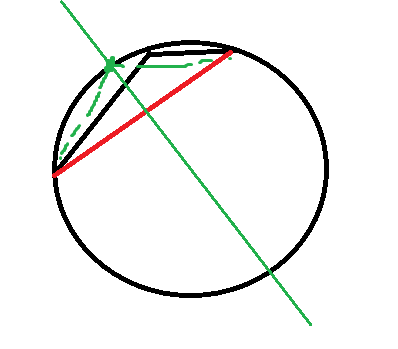
\includegraphics[scale=0.5]{../images/npolygon.png}
\end{center}

Короче, на данном моменте мы убедились, что максмальная площадь вписанного $n$-угольника достигается при его \Maleправильности\Male. Теперь осталось убедиться, что этот максимум вообще достигается.

Заведём функцию для площади многоугольника через центральные углы:

\[S(x) =  S(\alpha_1, \alpha_2 \ldots \alpha_n) = \sum_{i = 1}^n{\frac{1}{2}R\sin\alpha_i}\]

Тогда, заметим, что $0 \le \alpha_i \le \pi$, а так же функцию мы сотворили путём проведения преобразований над элементарными функциями (непрерывными) $\sin \alpha \rightarrow R\sin\alpha \rightarrow \sum_{i = 1}^n{\frac{1}{2}R\sin\alpha_i}$ то и наша функция является непрерывной (по арифм. свойствам). Заметим также, что множество наших векторов аргументов ограничено. Так же оно замкнуто (у нас все ограничения нестрогие). Поэтому множество аргументов --- компакт. А значит, его образ --- тоже и достигает максимума.

$\lhd$

\subsubsection{Лемма о связности отрезка\texorpdfstring{$^2$}{}}

\textbf{Формулировка}

$\langle a, b\rangle \subset \mathbb{R}$ --- отрезок. Тогда неверно, что $\exists V, U \subset{R}$ --- открытые множества, такие что:

\begin{enumerate}
    \item $U \cap V = \varnothing, U \neq \varnothing, V \neq \varnothing$
    \item $\langle a, b\rangle \subset U \cup V$
    \item $\langle a, b\rangle \cap U \neq \varnothing$ и $\langle a, b\rangle \cap V \neq \varnothing$
\end{enumerate}

\textbf{Доказательство}

$\rhd$

От противного. Пусть $\langle a, b\rangle \subset U \cup V, \alpha \in \langle a, b\rangle \cap U, \beta \in  \langle a, b\rangle \cap V$. Тогда пусть $\alpha < \beta$ (\Maleне умоляя общности\Male).Теперь положим $t = \sup{y : [\alpha, y) \subset U}$. Заметим, что множество, из которого мы берём экстремум непустое ($U \neq \varnothing, U$ --- открытое $\rightarrow \exists [\alpha, y) \subset B_\alpha \subset U$) и ограниченное ($U \cap V = \varnothing, y \in U \Rightarrow y < \beta$). Причём, раз $t \in [\alpha, \beta) \Rightarrow \langle a, b\rangle$. Если $t \in U \Rightarrow \exists V_t \subset U$, а мы строили множество границ так, что не существует такой окрестности. Если $t \in V$, то $\exists V_t \subset V$. Но тогда не весь промежуток $[\alpha, \beta)$ входит внутрь $U$, т.к. мешает как раз вот эта $V_t$. Следовательно, существуют точки, которые не накрываются ни одним отрезком.

$\lhd$

\subsubsection{Теорема о бутерброде\texorpdfstring{$^2$}{}}

\textbf{Формулировка}

Кусок колбасы и хлеба (фигуры $A, B \subset \mathbb{R}^2$) можно разрезать ножом (прямой) на части равной площади.

\textbf{Доказательство}

Сформулируем и докажем сначала лемму:

$A \subset \mathbb{R}^2, \Vec{V}$ --- произвольный вектор. Тогда существует прямая с направлением вектора $V$, которая делит прямую на 2 равновеликих фигуры.

$\rhd$

Давайте заведём числовую ось, причём эта ось пусть будет непараллельна $V$. Тогда $\forall t \in Ox : S(x) = S_l - S_r$. Будем через каждую точку числовой прямой $t$ будем проводить прямую, параллельную вектору $V$, и тогда для каждой такой точки будет определена функция как разность площадей левой и правой части фигуры.

\begin{center}
    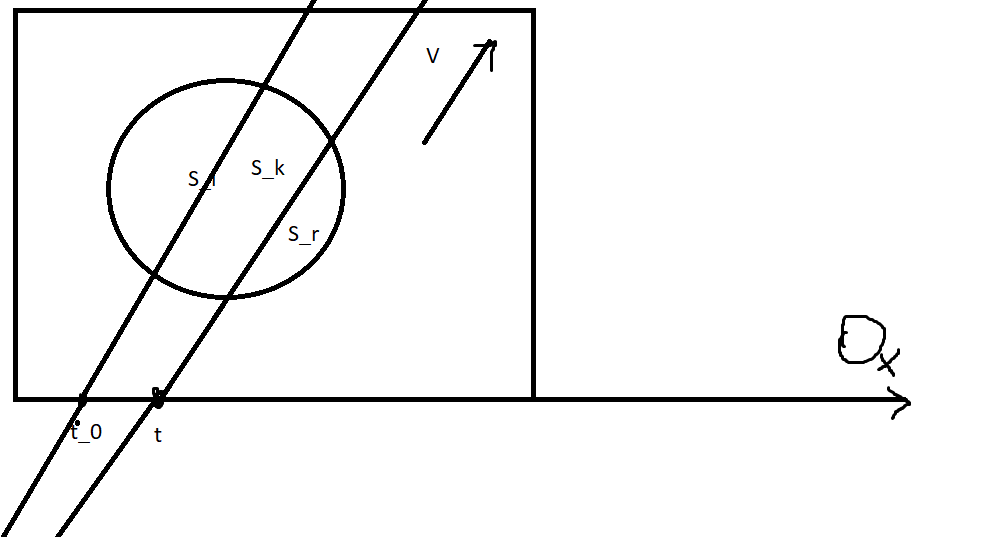
\includegraphics[scale=0.44]{../images/sandwich.png}
\end{center}

Заметим, что $|S(t_0) - S(t)| = |2S_k| \le (t - t0)h_{\text{доски}} \Rightarrow S(t)$ --- непрерывна, следовательно, между $-S$ и $S$ обязательно найдётся точка, в которой $S(t) = 0$ (по теореме о промежуточном значении).

$\lhd$

Теперь введём функцию $g(\varphi) = S^B_l(\varphi) - S^B_r(\varphi)$, это такая функция, которая определена на $\varphi \in [0, 2 * \pi]$ и проводит линию под углом $\varphi$ к оси координат, причём эта линия делит фигуру $A$ на равновеликие части.

Тогда, заметим что

\begin{enumerate}
    \item $g(\varphi + \pi) = -g(\varphi)$ (направление меняется, соответственно, меняется понятие лева и права)
    \item $g(\varphi_1) - g(\varphi_2) \le 4 * \frac{1}{2} * d^2 * |\sin \varphi_1 - \sin \varphi_2|$ (по сути, тоже площадь кусочка) $\Rightarrow g$ --- непрерывна.
\end{enumerate}

Тогда по теореме Больцпно-Коши о промежуточном значении всё получается!


\subsubsection{Теорема о сохранении промежутка\texorpdfstring{$^1$}{}}
\label{СохрПромеж}

\paragraph{Лемма}
\subparagraph{Формулировка}
$E$ выпукло $\Leftrightarrow$ $E$ промежуток

\subparagraph{Доказательство}
$\Leftarrow$ очевидно

$\Rightarrow$

$\letus M = \sup E, m = \inf E$

По определению $\sup$, в любой окрестности будут элементы множества. Таким образом, $(m, M) \subset E$. Также, поскольку $m$ и $M$ ограничивают выпуклое множество, $E \subset [m, M]$. Таким образом, $E$ - промежуток. 

\subparagraph{Формулировка}
Непрерывный образ промежутка --- промежуток. 

\subparagraph{Доказательство}
$f: C(\langle a, b \rangle \rightarrow \mathbb{R})$

$D := \langle a, b \rangle, f(D) = E$. $E$ выпукло по теореме о промежуточном значении (для любого отрезка на промежутке $\langle a, b \rangle$ теорема работает). 

Тогда, очевидно, $E$ --- промежуток. (по лемме чуть выше)


\subsubsection{Теорема Больцано--Коши о сохранении линейной связности\texorpdfstring{$^1$}{}}
\subparagraph{Линейная связность}
Множество в метрическом пространстве называется линейно связным, когда межу любыми 2 точками существует путь.

\subparagraph{Формулировка}
Непрерывный образ линейно-связного множества линейно-связен

\subparagraph{Доказательство}
$f: C(X \rightarrow Y)$, $X, Y$ -- метрические пространства.

$f(D) = E$. $D$ линейно-связно. $\Rightarrow \forall a, b \exists $ путь $g : C([0, 1] \rightarrow D)$, при этом $g(0) = a, g(1) = b$. 

Поскольку образ $g \subset D$, то $\forall x \in [0, 1] \exists f(g(x)) \in E$. При этом $f(g(0)) = f(a), f(g(1)) = f(b)$, то есть это работает для всех точек в $D$ 


\subsubsection{Описание линейно связных множеств в R\texorpdfstring{$^2$}{}}

\textbf{Определения}

$\gamma: [a, b] \rightarrow Y$ --- метрическое пространство. Тогда $\gamma$ --- путь в м.п. $Y$.

$E \subset Y$ --- метрическое пространство, тогда $E$ называется \textit{линейно связным}, если $\forall A, B \in E \dbl \exists \gamma: [a, b] \rightarrow E \text{ непрерывный}, \gamma(a) = A, \gamma(b) = B$

\textbf{Формулировка}

В $\mathbb{R} E$ --- линейно связно $\Leftrightarrow$ $E$ --- промежуток.

\textbf{Доказательство}

$\rhd$

$\Leftarrow$

Очевидно.

Что, не очевидно? А вот так? $t \in [0, 1], t(B - A) \subset [A, B] \subset \langle a, b \rangle$

$\Rightarrow$

$E$ --- не пустое (пустое --- тривиальный случай). Пусть $m = \inf E, M = \sup E$. Проверим, что $(m, M) \subset E$. $t \in (m, M), t \notin E$. Если возьмём $A, B \in E$ такие, что $m \le < A < t < B \le M$. Но в таком случае, $E$ не будет линейно связанным, т.к. $\exists c : \gamma: (a, b) \rightarrow E, \gamma(c) = t$. Тогда $(m , M) \subset E$.

$\lhd$


\subsubsection{Теорема о существовании и непрерывности обратной функции\texorpdfstring{$^1$}{}}
\subparagraph{Формулировка}
$f: C(\langle a, b \rangle \rightarrow \mathbb{R})$

$f$ строго монотонна (положим, возрастает)

Тогда $\exists f^{-1}$ и она строго возрастает и непрерывна

\subparagraph{Доказательство}
$\rhd$
\begin{enumerate}
\item
По определению обратной функции, $f$ обратима, когда является инъекцией. Поскольку $f(\langle a, b \rangle) = \langle m, M \rangle$, где $m = \inf$, $M = \sup$. Ну по \nameref{СохрПромеж}.

Поскольку $f$ строго возрастает, каждое значение на $\langle m, M \rangle$ принимает ровно 1 раз. Тогда это инъекция $\Rightarrow f$ обратима.

\item
Строгая монотонность обратной функции крайне очевидна:
$$
\forall x_1 > x_0 \quad f(x_1) > f(x_0) \Rightarrow \forall y_1 > y_0 \exists x_1 = f^{-1}(y_1), x_0 = f^{-1}(y_0)
$$
Т.к. $f^{-1}$ --- биекция, пара $x_1$ и $y_1$ однозначно определена и, следовательно, сохраняется неравенство $x_1 > x_0$

\item
По определению обратной функции, она является биекцией $\langle m, M\rangle$ в $\langle a, b \rangle$. Так как она монотонна, а её множество определения и значений --- промежутки, то она непрерывна (по \nameref{НепрМонФун}, п.2) 
\end{enumerate}
$\lhd$

\subsubsection{Равносильность двух определений производной. Правила дифференцирования.\texorpdfstring{$^3$}{}}

\paragraph{Равносильность определений дифференцируемости}

\textit{Формулировка: }

Определения дифференцируемости  (внезапно) равносильны

\begin{proof}
\item{$2 \Rightarrow 1$}
т.е. $f(x) = f(x_0) + A(x-x_0) + \varphi(x)(x-x_0)$, где $\varphi(x) \xrightarrow[x\to x_0]{}0$
Теперь все это разносим в разные стороны, делим на $x - x_0$ и получаем 
\begin{equation}
\frac{f(x) - f(x_0)} {x - x_0} = A + \varphi(x) \xrightarrow[x\to x_0]{} A \notag
\end{equation}
Что равносильно определению 1.
\item {$1 \Rightarrow 2$}
Обратно, обозначим 
\begin{equation}
\varphi(x) = \frac{f(x) - f(x_0)} {x - x_0} - A \notag
\end{equation}
Тогда $\varphi(x) \xrightarrow[x\to x_0]{}0$ и выполнено определение 2.
\end{proof}

\paragraph{Производная сумммы и разности}

\textit{Формулировка: }

$(f\pm g)' = f' \pm g'$

\begin{proof}
\begin{equation}
(f\pm g)' = \frac{(f+g)(x+\Delta x) - (f+g)(x)}{\Delta x} = \frac{f(x + \Delta x) - f(x)}{\Delta x} + \frac{g(x + \Delta x - g(x)} {\Delta x} \xrightarrow[\Delta x \to 0]{} f' \pm g' \notag
\end{equation}
\end{proof}

\paragraph{Производная сумммы и разности}

\textit{Формулировка: }

$(fg)'(x) = f'(x)g(x) + f(x)g'(x)$

\begin{proof}
\begin{eqnarray}
\frac{(fg)(x + \Delta x) - (fg)(x)} {\Delta x} = \frac{f(x + \Delta x) - f(x)} {\Delta x} g(x + \Delta x)+ \notag\\
+ f(x) \frac{g + \Delta x) - g(x)} {\Delta x} \xrightarrow[h\to 0] f'(x)g(x) + f(x)g'(x)\notag
\end{eqnarray}
\end{proof}

\paragraph{Производная частного}

\textit{Формулировка: }

$\left(\frac{f}{g}\right)' = \frac{f'(x)g(x) - f(x)g'(x)}{g^2(x)}$

\begin{proof}
\begin{eqnarray}
\frac{\frac{f}{g}(x + \Delta x) - \frac{f}{g}(x)}{\Delta x}=\frac{1}{g(x + \Delta x)(g(x)} \big(\frac{f(x + \Delta x) - f(x)} {\Delta x} g(x) - f(x) \frac{g(x+ \Delta x) - g(x)} {\Delta x}\big) \xrightarrow[h\to 0]{}\notag \\
\xrightarrow[h\to 0]{} \frac{f'(x)g(x) - f(x)g'(x)}{g^2(x)}\notag
\end{eqnarray}
\end{proof}

\paragraph{Производная композиции}

\textit{Формулировка: }

$(f \circ g)'(x) = g'(f(x)) * f'(x)$

\begin{proof}
Из определения 2 можно записать
\begin{eqnarray}
&f(x + \Delta x)=f(x) + f'(x)\Delta x + \alpha(\Delta x)\Delta x \notag \\
&g(y + \Delta y)=g(y) + g'(y)\Delta y + \beta(\Delta y)\Delta y \notag
\end{eqnarray}
где $\alpha$ и $\beta$ в нуле непрерывны и равны нулю. Во второе уравнение подставим\\ $\Delta y = f'(x)\Delta x + \alpha(\Delta x)\Delta x = \tau(\Delta x)$
\begin{eqnarray}
g(f(x + \Delta x)) &=& g(f(x)) + g'(f(x))\big(f'(x)\Delta x + \alpha(\Delta x)\Delta x\big) + \beta(\tau(\Delta x))\tau(\Delta x) =\notag\\
&=& g(f(x)) + g'(f(x))f'(x)\Delta x + \gamma(\Delta x)\Delta x \notag
\end{eqnarray}
где
\begin{equation}
\gamma (\Delta x) = g'(y)\alpha(\Delta x) + \beta(\tau(\Delta x)) \big(f'(x) + \alpha(\Delta x)\big)\notag
\end{equation}
Ясно, что $\gamma(0) = 0, \gamma$ непрерывна в нуле, следовательно, $f \circ g$ дифференцируема в 0 и выполняется требуемое в условии.
\end{proof}

\paragraph{Производная обратной функции}

\textit{Формулировка: }
$(f^{-1})'(f(x)) = \frac{1} {f'(x)}$

\begin{proof}
Вот здесь начинается веселье. Из предыдущих теорем курса мы знаем, что$ f^{-1}$ существует, определена на $P$, строго монотонна и непрерывна. Пусть $y = f(x)$, возьмем $\Delta y \neq 0: y + \Delta y \in P$, положим $\Delta x = f^{-1}(y + \Delta y) - f^{-1}(y) = \tau(\Delta y)$. Тогда $\Delta x \neq 0, x = f^{-1}(y),  x + \Delta x = f^{-1}(y + \Delta y)$ и $f(x + \Delta x) - f(x) = \Delta y$. Составим разностное отношение
\begin{equation}
\frac{f^{-1}(y + \Delta y) - f^{-1}(y)} {\Delta y} = \frac{\tau(\Delta y)} {f(x + \tau(\Delta y)) - f(x)} \notag
\end{equation}
и найдем его предел при $\Delta y \to 0$. По условию ($f$ - дифференцируема)
\begin{equation}
\frac{\Delta x} {f(x + \Delta x) - f(x)} \xrightarrow[h\to 0]{} \frac{1} {f'(x)}\notag
\end{equation}
Но $\tau(k) \xrightarrow[k\to 0]{} 0$ по непрерывности $f^{-1}$ в точке $y$ 	 . Следовательно, по теореме о пределе композиции
\begin{equation}
\frac{f^{-1}(y + \Delta y) - f^{-1}(y)} {\Delta y} \xrightarrow[k\to 0]{} \frac{1} {f'(x)}\notag
\end{equation}
\end{proof}

\subsubsection{Теорема Ферма (с леммой)\texorpdfstring{$^2$}{}}

\textbf{Формулировка (Лемма)}

$f: \langle a, b \rangle \rightarrow \mathbb{R}$, дифференцируема и возрастает в т. $x_0 \in (a, b)$. Тогда $f^\prime(x_0) > 0, \exists \varepsilon > 0 : \forall x \in (x_0 - \varepsilon, x_0) \dbl f(x) < f(x_0)$ и $(x_0, x_0 + \varepsilon) \dbl f(x) > f(x_0)$ (строго возрастает).


\textbf{Доказательство (Лемма)}

Во-первых, $\lim_{x \rightarrow x_0}{\frac{f(x) - f(x_0)}{x - x_0}} = f^\prime(x_0) > 0$

Тогда, по теореме о стабилизации знака:

$x \rightarrow x_0 + 0$ (справа), тогда $f(x) - f(x_0) > 0$

$x \rightarrow x_0 + 0$ (слева), тогда $f(x) - f(x_0) < 0$

Сошлось (вблизи $x_0$).

\textbf{Формулировка (Теорема)}

$f: \langle a, b \rangle \rightarrow \mathbb{R}$, дифференцируема в т. $x_0 \in (a, b), c = \max_{x \in (a, b)} f(x)$. Тогда $f^\prime(x_0) = 0$.

\textbf{Доказательство (Теорема)}

$\rhd$

$f(x) - f(c) \le 0$

$f^\prime(x) = \lim_{x \rightarrow c}\frac{f(x) - f(c)}{x - c}$. Заметим, что $x = c + \Delta x$. Тогда $\lim_{\Delta x \rightarrow 0}{\frac{f(c + \Delta x)}{\Delta x}} = f^\prime(c)$

$\lim_{x \rightarrow c - 0}\frac{f(x) - f(c)}{x - c} \ge 0 \Rightarrow f^\prime \ge 0$

$\lim_{x \rightarrow c + 0}\frac{f(x) - f(c)}{x - c} \le 0 \Rightarrow f^\prime(c) \le 0$

(Всё дело в знаменателе!!!!)

Тогда $0 \le f^\prime(x) \le 0 \Rightarrow f^\prime(c) = 0$

$\lhd$

\subsubsection{Теорема Ролля. Вещественность корней многочлена Лежандра\texorpdfstring{$^2$}{}}

\paragraph{Теорема Ролля}
\textbf{Формулировка}

$f: [a, b] \rightarrow \mathbb{R}$, дифференцируема на $(a, b)$ и непрерывна на $[a, b], f(a) = f(b)$. Тогда $\exists c: f^\prime(x) = 0$

\textbf{Доказательство}

$\rhd$

По теореме Вейерштрасса, $\exists x_0 = \min_{x \in [a, b]}{f(x)}, x_1 = \max_{x \in [a, b]}{f(x)}$. Тогда, по теореме Ферма, если $x_0$ или $x_1$ лежит в $(a, b)$, то нам подходит $c = x_0$ или $c = x_1$. Иначе, если $x_0 = x_1 \Rightarrow$ const. Если не лежит в $(a, b) \Rightarrow x_0 = a, x_1 = b \Rightarrow$ const, тривиально.

$\lhd$

\textit{Следствие}

$f: [a, b] \rightarrow \mathbb{R}$, непрерывна на $[a, b], f(a) = f(b) = 0 \Rightarrow \exists c \in (a, b)$

\paragraph{Вещественность корней многочлена Лежандра}
\textbf{Формулировка}

$L_n(x) = \left((x^2-1)^n\right)^{(n)}$ --- многочлен Лежандра.

Утверждается, что он имеет $n$ вещественных корней на $(-1, 1)$.

\textbf{Доказательство}

$\rhd$

Корень $a$ называется корнем кратности $k$ исходной функции $f(x)$, если $f_1(x) = (x - a)^kf_1(x)$ и $f_1(a) \neq 0$. Заметим, что если $a$ корень кратности $k$ для $f(x)$, то для $f^\prime(x)$ это корень кратности $k - 1$ (доказывается дифференцированием $(x - a)^kf_1(x)$).

Тогда поехали. Для самого многочлена Лежандра существует 2 корня кратности $n: {1, -1}$. Если взять производную, то по теореме Ролля $\exists c \in (a, b)$, следовательно, существует ещё один корень. Наши же первоначальные корни остаются корнями уравнения, но их кратность стала по $n-1$. Тогда всего в сумме у нас получается $2n - 2 + ?$ корней, где $? = 1$, т.к. вообще корней у многочлена первой производной существует не более $2n - 1$. Так продолжаем и дальше, в итоге получаем, что у $k$-й производной есть $k$ корней. Тогда для производной степени $n$ у многочлена Лежандра $n$ вещественных корней.

$\lhd$

\subsubsection{Непрерывность синуса и арксинуса, замечательный предел, производная синуса.\texorpdfstring{$^3$}{}}

\paragraph{Лемма}

\textit{Формулировка: }

$\forall x \in \mathbb{R}$
\begin{equation}
|\sin{x}| \leq |x| \notag
\end{equation}

\paragraph{Непрерывность синуса}

\textit{Формулировка: }

Синус непрерывен на $\mathbb{R}$

\begin{proof}
$\forall x+0 \in \mathbb{R}$
\begin{equation}
\left|\sin{x} - \sin{x_0}\right| = \left|2\sin{\frac{x - x_0} {2}} \cos{\frac{x + x_0} {2}}\right| \leq 2 *  \frac{|x - x_0|} {2} * 1 = |x - x_0| \xrightarrow[x\to x_0] {} 0\notag
\end{equation}
\end{proof}

$\arcsin{}: [-1, 1] \xrightarrow{\text{на}} \left[ -\frac{\pi}{2}, \frac{\pi}{2}\right]$ непрерывна по теореме о непрерывности обратной функции

\paragraph{Первый замечательный предел} \label{first_lim}

\textit{Формулировка: }

\begin{equation}
\lim_{x\to 0} \frac{\sin{ x}} {x} = 1 \notag
\end{equation}

\begin{proof}
При $x \in \left( 0, \frac{\pi}{2}\right)$
\begin{equation}
\sin{x} < x < \tg{x}\notag
\end{equation}
Делим это все на $\sin{x}$ и берем обратные, из-за чего неравенство переворачивается, и получаем
\begin{equation}
\cos{x} < \frac{\sin{x}}{x} < 1\notag
\end{equation}
т.к. все части этого неравенства --- четные функции, то такой переход легитимен. А т.к. $\cos{x}$ стремится к 1 при $ x\to 0$, то по теореме о зажатой функции --- победа.
\end{proof}

\paragraph{Производная синуса}

\textit{Формулировка: }

$(\sin{x})' = \cos{x}$

\begin{proof}
Пользуемся замечательным пределом выше и непрерывностью косинуса
\begin{equation}
\frac{\sin{x + \Delta x} - \sin{x}} {\Delta x} = \frac{2\sin{\frac{\Delta x} {2}} \cos{\left( x + \frac{\Delta x} {2} \right)}} {\Delta x} \xrightarrow[\Delta x \to 0] {} \cos{x} \notag
\end{equation}
\end{proof}
\newpage



\section{Период 3 (Кайнозойский)}
\subsection{Важные определения}

\subsubsection{Множество мощности континуума\texorpdfstring{$^1$}{}}
Множество мощности континуума равномощно $[0, 1] \subset \mathbb{R}$


\subsubsection{Разложения Тейлора основных элементарных функций\texorpdfstring{$^1$}{}}
$$
e^x = 1 + x + \frac{x^2}{2!}+\ldots+\frac{x^n}{n!}+o(x^n)
$$
$$
\sin{x} = x - \frac{x^3}{3!} + \frac{x^5}{5!} + \ldots + (-1)^n\frac{x^{2n+1}}{(2n+1)!} + o(x^{2n+1})
$$
$$
\cos{x} = 1 - \frac{x^2}{2!} + \frac{x^4}{4!} + \ldots + (-1)^n\frac{x^{2n}}{(2n)!} + o(x^{2n})
$$
$$
\ln{(1 + x)} = x - \frac{x^2}{2} + \frac{x^3}{3} - \frac{x^4}{4} + \ldots + (-1)^{n+1}\frac{x^n}{n} + o(x^n)
$$
$$
(1+x)^\alpha = 1 + \alpha x + \frac{\alpha (\alpha - 1)}{2!}x^2 + \frac{\alpha(\alpha-1)(\alpha-2)}{3!}x^3 + \ldots + \binom{\alpha}{n}x^n + o(x^n)
$$


\subsubsection{Выпуклая функция и касательная\texorpdfstring{$^{1 \ 3}$}{}}
$f : \langle a, b\rangle \rightarrow \mathbb{R}$ - выпуклая $\Leftrightarrow$
$$
\forall x, y \in \langle a, b \rangle \quad \forall \alpha \in (0, 1) \quad f(\alpha x + (1-\alpha)y) \le \alpha f(x)+(1-\alpha) f(y)
$$

Вообще это утверждение эквивалентно неравенству Йенсена. Смысл в том, что мы можем зафиксировать любые 2 точки $x$ и $y$ на указанном отрезке, при чём будет верно то, что если мы соединим их прямой (ну то есть получим хорду из $(x, f(x)$ в $y, f(y)$), то эта хорда будет выше, либо равна нашей функции (ну то есть функция как-то идёт сначала вниз, а потом начинает расти и пересекает хорду только в точке $y$. 

Аналогично, есть "вогнутая" функция ($\Leftrightarrow$ "выпуклой сверху").

Также, можем ввести "строго выпуклую функцию". Определение такое же, но хорда должна быть строго выше.

\subsubsection{Теорема Дарбу. Следствия\texorpdfstring{$^3$}{}}

\paragraph{Теорема Дарбу}

\textit{Формулировка: }
    $f$ -  дифференцируема на $[a, b] \Rightarrow \forall C \in (f'(a), f'(b)) \exists c \in (a, b): f'(c) = C$

    \begin{proof}
    \item{1. $f'(a)$ и $f'(b)$ разных знаков, $C = 0$.\\}
    НУО $f'(a) < 0 < f'(b)$. Т.к. $f$ непрерывна на $[a, b]$ то по Вейерштрассу $\exists c \in [a, b]: f(c) = \min_{x\in [a,b]} f(x)$. Если $c\in (a, b)$, то из Ферма $f'(c) = 0$ --- победа. Проверим, что $c \neq b$ и $c \neq a$. Если $c = a$, то $\forall x \in (a, b] \frac{f(x) - f(a)}{x - a} \geq 0 \Rightarrow f'(a) \geq 0$. Противоречие с условием. Аналогично, $c \neq b$
    \item{2. Общий случай\\}
    НУО  $f'(a) < C < f'(b)$. $\varphi(x) = f(x) - Cx$. Тогда 
    \begin{equation}
    \varphi'(a) = f'(a) - C < 0 < f'(b) - C = \varphi'(b) \notag
    \end{equation}
    Из 1. $\Rightarrow \exists c \in (a, b): \varphi'(c) = 0$, т.е. $f'(c) = C$ 
    \end{proof}

\paragraph{Лемма о характеристике промежутков}

\textit{Формулировка: }

    $E \subset \mathbb{R}$. Тогда следующие утверждения равносильны.

    \begin{enumerate}
        \item E --- промежуток
        \item $\forall x,y \in E, [x, y] \subset E$
    \end{enumerate}

    \begin{proof}
    \item{$1. \Rightarrow 2.$} 
    Очевидно
    \item{$2. \Rightarrow 1.$}
    Пусть $E \neq \emptyset$. Обозначим $m$ = inf $E$, $M$ = sup $E$. Очевидно, $E \subset [m, M]$. Покажем, что $(m, M) \subset E$. Пусть $m < z < M$. Тогда из определения граней $\Rightarrow \exists x, y \in E: x < z < y$ По условию $z \in E$
    \end{proof}

    \paragraph{Следствие 1}

    \textit{Формулировка: }

    $f$ --- дифференцируема на $\langle a, b\rangle \Rightarrow f'(\langle a, b\rangle)$ --- промежуток.

    \begin{proof}
    Следует из леммы о характеристике промежутков
    \end{proof}

    \paragraph{Следствие 2}

    \textit{Формулировка: }
    Производная дифференцируемой на промежутке функции не может иметь на нем разрывов второго рода

    \begin{proof}
    Аналогично доказательству теоремы о непрерывности монотонной функции
    \end{proof}

\newpage
\subsection{Определения}

\subsubsection{Классы функций \texorpdfstring{$C^n([a,b])$}{n-гладкое C([a, b])}\texorpdfstring{$^1$}{}}
$f$ называется $n$-гладкой, если имеет $n$ непрерывных производных (формально, $\forall i = 1\ldots n \; \exists \; i$-ая непрерывная производная)

Класс функций $C^n([a,b])$ - это множество $n$-гладких функций на $[a,b]$


\subsubsection{Производная \texorpdfstring{$n$}{n}-го порядка\texorpdfstring{$^1$}{}}
Пусть есть натуральное $n$. $f: X \rightarrow Y$ (где $X$ и $Y$ - м.п.) - дифференцируема в интервале $(a, b)$. Тогда мы можем взять производную $f'(x)$ в этом интервале. Далее индуктивно мы можем рассуждать о полученной производной как о функции. 

Такими темпами мы дойдём до $f^(n)$, что и называют "производной $n$-го порядка"


\subsubsection{Многочлен Тейлора \texorpdfstring{$n$}{n}-го порядка\texorpdfstring{$^1$}{}}
$T_n(f, a)(x) = f(a) + \frac{f'(a)}{1!}(x-a)  + \frac{f''(a)}{2!}(x-a)^2 + \ldots+ \frac{f^{(n)}(a)}{n!}(x-a)^n$


\subsubsection{Счётное множество\texorpdfstring{$^1$}{}}
Множество счётно $\Leftrightarrow$ множество равномощно $\mathbb{N}$. 
То есть можно установить биекцию между $\mathbb{N}$ и множеством


\subsubsection{Выпуклое множество в \texorpdfstring{$\mathbb{R}^m$}{m-мерном R}\texorpdfstring{$^1$}{}}
$A \subset \mathbb{R}^m$ - выпуклое множество в $\mathbb{R}^m$, если 
$$
\forall x, y \in A, \alpha \in [0, 1] \quad \alpha x + (1 - \alpha) y \in A
$$
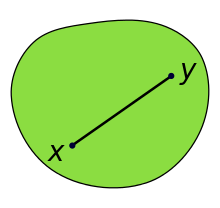
\includegraphics[scale=0.9]{convex}
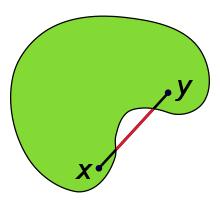
\includegraphics[scale=0.9]{non-convex}


\subsubsection{Надграфик\texorpdfstring{$^1$}{}}
Надграфик функции $f: \langle a, b \rangle \rightarrow \mathbb{R}$ это множество $\{(x, y)|x\in \langle a, b\rangle, y \ge f(x)\}$


\subsubsection{Опорная прямая\texorpdfstring{$^1$}{}}
$A \subset \mathbb{R}^2$ - выпуклое
$l \subset \mathbb{R}^2$ - прямая

$l$ - опорная прямя для $A$, когда выполняется:
\begin{enumerate}
    \item $A$ содержится в одной полуплоскости относительно $l$ (лежит полностью по одну сторону от прямой)
    \item Пересечение прямой и множества непусто ($l \cap A \ne \varnothing$)
\end{enumerate}
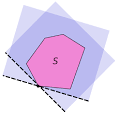
\includegraphics{baseline}


\subsubsection{Равномерная непрерывность\texorpdfstring{$^1$}{}}
Равномерность непрерывности говорит то, что мы можем для $\varepsilon$ найти конкретный $\delta$, который не зависит от аргументов (работает на всей области определения), при котором разность значения функции меньше $\varepsilon$

Формально, 
$$
\forall \varepsilon > 0 \hspace{5pt} \exists \delta > 0 \hspace{5pt} \forall x_1, x_2 \in \langle a, b \rangle : |x_1 - x_2| < \delta \quad |f(x_1) - f(x_2)| < \varepsilon 
$$

Аналогично, это работает для метрических пространств:
$$
\forall \varepsilon > 0 \hspace{5pt} \exists \delta > 0 \hspace{5pt} \forall x_1, x_2 \in \langle a, b \rangle : \rho(x_1 - x_2) < \delta \quad \rho(f(x_1) - f(x_2)) < \varepsilon 
$$

\subsubsection{Локальный экстремум\texorpdfstring{$^3$}{}}
$f:D\subset \mathbb{R} \to \mathbb{R}$ $x_0 \in D$
\begin{enumerate}
\item $x_0 - $ точка локального максимума, если $\exists U(x_0) \forall x \in U(x_0) \cap D\quad f(x) \leq f(x_0)$
\item $x_0 - $ точка строгого локального максимума, если $\exists U(x_0) \forall x \in \dot U(x_0) \cap D\quad f(x) < f(x_0)$
\item Локальный минимум определяется аналогично
\item Локальный экстремум = локальный максимум или локальный минимум
\end{enumerate}

\newpage
\subsection{Важные теоремы}

\subsubsection{Формула Тейлора с остатком в форме Пеано\texorpdfstring{$^2$}{}}

\textbf{Формулировка}

Пусть $f(x)$ дифференцируема в точке $x_0 n$ раз, у неё есть многочлен Тейлора $P_n(x))$, тогда $f(x) = P_n(x) + o((x - x_0))^n$ при $x \rightarrow x_0$.

\textbf{Доказательство}

$\rhd$

У нас есть некое \textit{основное свойство многочлена Тейлора}, которое утверждает, что функция и её многочлен Тейлора $n$ степени, а также их производные до $n$ порядка включительно имеют равное значение в точке $x_0$. Запомним. Тогда определим остаток $R_n(x) = f(x) - P_n(x)$. Перефразируя условие, $R_n(x_0) = R_n^\prime(x_0) = \ldots = R_n^{(n)}(x_0) = 0$. Из непрерывности в точке $x_0$ также следует, что пределы функции $R_n(x)$ и её производных до $n$ при $x \rightarrow x_0$ порядка равны 0. Супер. Тогда нам по сути нужно доказать, что $R_n(x) = o(x - x_0)^n$ при $x \rightarrow x_0 \Leftarrow \lim_{x \rightarrow x_0}\frac{R_n(x)}{(x - x_0)^n}$. По-Лопиталим всё это дело $n - 1$ раз, и получим $\frac{1}{n!}\lim_{x \rightarrow x_0}\frac{R_n^{(n - 1)}(x) - R_n^{(n - 1)}(x_0) (= 0)}{(x - x_0)^n}$ --- а это определение производной $R_n^{(n)}(x) = 0$

$\lhd$

\subsubsection{Формула Тейлора с остатком в форме Лагранжа\texorpdfstring{$^1$}{}}
Определение:

$f \in C^n\langle a, b\rangle, (n+1)$ раз дифференцируема на $(a, b)$

$x, x_0 \in \langle a, b\rangle$. Тогда $\exists c$ между $x$ и $x_0$

$f(x) = f(x_0) + \frac{f'(x_0)(x-x_0)}{1!} + \ldots + \frac{f^{(n)} (x_0)}{n!} (x-x_0)^n + \frac{f^{(n+1)} (c)}{(n+1)!}(x-x_0)^{n+1}$

Доказательство:
$$
\phi(t) = f (x) - T_n(f, t)(x) = f(x) - \left(f(t) + \frac{f'(t)}{1!}(x-t) + \ldots + \frac{f^{(n)}(t)}{n!}(x-t)^n\right)
$$
$$
\phi(x) = 0 
$$
$$
\phi'(t) = -\left(f'(t)+\left(-\frac{f'(t)}{1!}+\frac{f''(t)}{1!}(x-t)\right)+\left(-\frac{f''(t)}{1!}(x-t)+\frac{f'''(t)}{2!}(x-t)^2\right) + \ldots\right) =
$$
$$
=-\frac{f^{(n+1)}(t)}{n!}(x-t)^n
$$

$\psi(t) := (x-t)^{n+1}$. По Т. Коши $\exists c$ между $x$ и $x_0:$
$$
\frac{-R_n(f, x_0)(x)}{-(x-x_0)^{n+1}} = \frac{\phi(x)-\phi(x_0)}{\psi(x)-\psi(x_0)} = \frac{\phi'(c)}{\psi'(c)} = \frac{-\frac{f^{(n+1)} (c) }{n!} (x-c)^n}{-(n+1)(x-c)^n}
$$
Тогда $R_n(f, x_0)(x) = \frac{f^{(n+1)}(x_0)+\theta(x-x_0)}{n!} (1-\theta)^n(x-x_0)^{n+1}$ - ост. в форме Коши

\newpage

\subsection{Теоремы}

\subsubsection{Следствие об оценке сходимости многочленов Тейлора к функции. Примеры\texorpdfstring{$^3$}{}}
\paragraph{Лемма}

\textit{Формулировка: }

Пусть выполнены условия для существования формулы Тейлора с остатком в форме Лагранжа, $M > 0, \forall t\in \langle x, x_0\rangle|f^{(n+1)}(t)| \leq M$. Тогда 
\begin{equation} \label{eq_a}
|R_{n, x_0} f(x)| \leq \frac{M|x - x_0|^{n+1}} {(n+1)!} 
\end{equation}

\begin{proof}
Прямо следует из формы Лагранжа остаточного члена.
\end{proof}

\paragraph{Следствие}

\textit{Формулировка: }

Пусть $f \in C^{(\infty)} \langle a, b\rangle$, и существует $M > 0: \forall n \in \mathbb{N} \text{ и } t \in \langle a, b\rangle$ выполняется неравенство $| f^{(n)}(t)| \leq M$. Тогда $\forall x, x_0 \in \langle a, b\rangle$
\begin{equation} \label{eq_b}
T_{n, x_0} f(x) \xrightarrow[n\to\infty]{}f(x)
\end{equation}

\begin{proof}
Т.к. $\forall K \in \mathbb{R}$ $ \frac{K^n} {n!} \xrightarrow[n\to\infty]{} 0$ и \eqref{eq_a} выполняется для всех $n$ одновременно, получаем $R_{n, x_0}f(x) \xrightarrow[n \to\infty]{} 0 \Leftrightarrow \eqref{eq_b}$
\end{proof}

\paragraph{Пример 1}

\textit{Формулировка: }

Остаток для $e^x$

\begin{proof}
Так как $(e^x)^{(k)} = e^x; (e^x)^{(k)} \arrowvert_{x=0} = 1$, верны равенства
\begin{eqnarray}
e^x = \sum_{k=0}^n \frac{x^k} {k!} + o(x^n) = 1 + x + \frac{x^2} {2} + \frac{x^3} {6} + \frac{x^4} {24} + \dots + \frac{x^n} {n!} + o(x^n),\notag\\
e^x = \sum_{k=0}^n \frac{x^k} {k!} + \frac{e^{\theta x}}{(n+1)!} x^{n+1}, \quad \theta \in(0, 1) \notag
\end{eqnarray}
В частности при $x = 1$
\begin{equation}
e = \sum_{k = 0}^n \frac{1} {k!} + \frac{e^\theta} {(n + 1)!}, \quad \theta \in (0, 1) \notag
\end{equation}
Отсюда получаем оценки 
\begin{eqnarray}
\left|e^x - \sum_{k=0}^n\frac{x^k}{k!}\right| \leq \frac{max\{e^x, 1\}} {(n+1)!} |x|^{n+1},\notag\\
\frac{1} {(n+1)!} < e - \sum_{k=0}^n \frac{1}{k!} < \frac {e} {(n+1)!} < \frac{3} {(n+1)!}\notag
\end{eqnarray}
Следовательно, $\forall x \in \mathbb{R}$
\begin{equation}
e^x = \lim_{n\to\infty} \sum_{k = 0}^n \frac{x^k} {k!}\notag
\end{equation}
и, в частности,
\begin{equation}
e = \lim_{n\to\infty}\sum_{k=0}^n \frac{1}{k!} \notag
\end{equation}
\end{proof}

\paragraph{Пример 2}

\textit{Формулировка: }

Остаток для $\sin{x}$

\begin{proof}
Из формулы 
\begin{equation}
(\sin{x})^{(m)} = \sin{\left(x + \frac{m\pi} {2}\right)}\notag
\end{equation}
при $k \in \mathbb{Z}_+$
\begin{equation}
(\sin{x})^{(2k)} \arrowvert_{x=0} = 0 \qquad (\sin{x})^{(2k + 1)} \arrowvert_{x=0} = (-1)^k\notag
\end{equation}
Поэтому 
\begin{eqnarray}
\sin{x} = \sum_{k=0}^n \frac{(-1)^k} {(2k+1)!} x^{2k+1} + o(x^{2n+2}) = x - \frac{x^3} {6} + \frac{x^5} {120} - \dots + \frac{(-1)^n} {(2n + 1)!} x^{2n+1} + o(x^{2n+2}),\notag \\
\sin{x} = \sum_{k=0}^n \frac{(-1)^k} {(2k+1)!} x^{2k+1} + \frac {\sin{\alpha}} {(2n+3)!} x^{2n+3}\notag
\end{eqnarray}
где $\alpha = \theta x + \frac{(2n + 3)\pi} {2}, \theta \in (0, 1)$.
Отсюда получаем оценку остатка
\begin{equation}
|R_{2n+2, 0} (sin, x )| \leq \frac{|x|^{2n + 3}} {(2n+3!)} \notag
\end{equation}
Поэтому $\forall x \in \mathbb{R}$
\begin{equation}
\sin{x} = \lim_{n\to\infty}\sum_{k=0}^n \frac{(-1)^k} {(2k+1)!} x^{2k+1}\notag
\end{equation}
\end{proof}

\paragraph{Пример 3}

\textit{Формулировка: }

Остаток для $\cos{x}$

\begin{proof}
\begin{equation}
(\cos{x})^{(m)} = \cos{\left(x + \frac{m\pi} {2}\right)}\notag
\end{equation}
\begin{equation}
(\cos{x}^{(2k)}\arrowvert_{x=0} = (-1)^k, \qquad (\cos{x})^{(2k + 1)} \arrowvert_{x=0} = 0\notag
\end{equation}
\begin{equation}
\cos{x} = \sum_{k=0}^n \frac{(-1)^k} {(2k)!} x^{2k} + o(x^{2n+1}) = 1 - \frac{x^2} {2} + \frac {x^4} {24} - \frac{x^6} {720} + \dots + \frac{(-1)^n} {(2n)!} x^{2n} + o(x^{2n+1}),\notag
\end{equation}
\begin{equation}
\cos{x} = \sum_{k=0}^n \frac{(-1)^k} {(2k)!} x^{2k} + \frac {\cos{\beta}} {(2n+2)!} x^{2n+2}\notag
\end{equation}
где $\beta = \theta x + \frac{(2n+2)\pi} {2}, theta \in (0, 1)$. Отсюда
\begin{equation}
|R_{2n+1, 0} (cos, x)| \leq \frac{|x|^{2n+2}}{(2n+2)!}\notag
\end{equation}
Поэтому, $\forall x \in \mathbb{R}$
\begin{equation}
\cos{x} = \lim_{n \to\infty}\sum_{k=0}^n \frac{(-1)^k} {(2k)!} x^{2k}\notag
\end{equation}
\end{proof}

\paragraph{Пример 4}

\textit{Формулировка: }
Остаток для $\ln{\left(1 + x\right)}$

\begin{proof}
Т.к. $\forall k \in \mathbb{N}$
\begin{equation}
(\ln{\left(1 + x\right)})^{(k)} = \frac{(-1)^{k-1}(k-1)!}{(1+x)^k}, \qquad (\ln{\left(1 + x\right)})^{(k)}\arrowvert_{x=0} = (-1)^{k-1}(k-1)!\notag
\end{equation}
а $\ln{1} = 0$, получаем
\begin{equation}
\ln{\left(1 + x\right)} = \sum_{k=1}^n \frac{(-1)^{k-1}}{k} x^k + o(x^n) = x - \frac{x^2} {2} + \frac{x^3} {3} - \frac{x^4} {4} + \dots + \frac{(-1)^{n-1} }{n} x^n + o(x^n)\notag
\end{equation}
\end{proof}

\subsubsection{Несчетность отрезка\texorpdfstring{$^3$}{}}
\textit{Формулировка: }
Отрезок несчетен: $\nexists \varphi:\mathbb{N} \to [0, 1]$

\begin{proof}
От противного. Пусть мы занумеровали все точки отрезка:$x_1, x_2, x_3, \ldots, x_n, \ldots$. Построим последовательность отрезков. $\Delta_0 = [0, 1]$. Делим $\Delta_0$ на три отрезка, пусть $\Delta_1$ --- та треть $\Delta_0$, что не содержит $x_1$. Продолжаем делить и брать трети:$\Delta_n$ --- треть $\Delta_{n-1}$, не содержащая $x_n$.

Очевидно, что $\Delta_0 \supset \Delta_1 \supset \ldots \supset \Delta_n \supset\ldots$. Но по теореме о стягивающихся отрезках $\cap \Delta_i = \{a\}$, но $a$ не совпадает ни с одним из $x_i$. Абсурд.
\end{proof}

\subsubsection{Континуальность множества бинарных последовательностей\texorpdfstring{$^3$}{}}
\textit{Формулировка: }

$Bin$ --- множество всех бесконечных последовательностей из 0 и 1. Тогда $\exists \varphi:[0,1] \to Bin$ --- биекция.

\begin{proof}
$x \in [0, 1]$ $x = 0.1011000010\ldots$. При отбрасывании целой части получаем бинарную последовательность. Однако существуют $x$, задающиеся двумя бинарными последовательностями: Те, у которых, начиная с $k$-й позиции идут только единицы и те, у которых в $(k-1)$-й позиции 1, а начиная с $k$-й только нули. Но таких последовательностей, очевидно, счетное число. Понятно, что объединение континуального и счетного множества континуально.
\end{proof}

\subsubsection{Теорема о свойствах показательной функции\texorpdfstring{$^1$}{}}
\textit {Напоминалка}

Показательная функция $f:\mathbb{R}\to\mathbb{R}$ --- по определению: непрерывна, не тождественный 0, не тождественная 1, и $f(x + y) = f(x) \cdot f(y)$

Формулировка:
\begin{enumerate}
    \item $\forall x f(x) > 0; f(0) = 1$
    \item $\forall r \in \mathbb{Q} \quad f(rx) = (f(x))^r$
    \item Пусть $a:= f(1)$, тогда \\$a=1 \implies f-const$, $a > 1 \implies f \text{- возр.}$, $a < 1 \implies f \text{- убыв.}$
    \item Множество значений $f$ $\rightarrow (0, +\infty)$
    \item $\tilde f(1) = f(1)$, тогда $f = \tilde f$
\end{enumerate}
Доказательство:
\begin{enumerate}
    \item $\exists x_0 \quad f(x_0) \ne 0\\ f(x_0+0) = f(x_0) f(0) \implies f(0) = 1$\\
    Если $\exists x_1: f(x_1) = 0 \; \forall x \quad f(x) = f(x-x_1)f(x_1)=0$, т.е. $f\equiv 0$\\
    Тогда $\forall x \quad f(x) = f(\frac{x}{2})f(\frac{x}{2}) > 0, f(x) \ne 0$
    
    \item \begin{enumerate} 
        \item $r = 1 \hfill$ Тривиально
        \item $r \in \mathbb{N}$ 
        \begin{align}
        f(2x) = f(x+x) = f(x) f(x) = f(x^2)\\
        f((n+1)x)=f(nx+x)=f(nx)f(x)=(f(x))^nf(x)=(f(x))^{n+1}
        \end{align}
        
        \item $r \in -\mathbb{N} \hfill 1=f(0)=f(nx+(-n)x)=f(nx)f(-nx)=(f(x))^nf(-nx)$
        
        \item $r = 0 \hfill f(rx) = f(0) = 1 = (f(x))^0$
        
        \item $r=\frac{1}{n}$
        \begin{align}
        f(x)=f(n\frac{x}{n})=(f(\frac{x}{n}))^n\\
        f(\frac{1}{n}x)=(f(x))^{\frac{1}{n}}
        \end{align}
        
        \item $r=\frac{m}{n}, m\in \mathbb{Z}, n \in \mathbb{N} \hfill f(rx) = f(x\frac{m}{n}) = (f(\frac{x}{n}))^m=((f(x))^\frac{1}{n})^m$
    \end{enumerate}

    \item $a=1 \quad f(1)=1 \quad \forall r \in \mathbb{Q} \; f(r) = 1^r = 1$\\
    $f$ - непр. и $f(x) = 1$ при $x \in \mathbb{Q} \implies f \equiv 1$ \\
    $a > 1$. Тогда $\forall x > 0 \quad f(x) > 1$ \\
    $r \in \mathbb{Q}, r > 0 \quad f(r) = r(r*1) = (f(1))^r=a^r>1$\\
    Значит $\forall x \in \mathbb{R}, x > 0$ берем $r_k \rightarrow x(r_k \in \mathbb{Q})$\\
    $f(r_k) \rightarrow f(x)$, значит $f(x) \ge 1$\\
    $f(x) = f((x-r)+r)=f(x-r)*f(r) > 1$\\
    $\exists r \in \mathbb{Q} : 0 < r < x$\\
    Возр. $x \in \mathbb{R}, h > 0$\\
    $f(x+h) = f(x) f(h)$\\
    $f(h) > 1 \implies f(x+h) > f(x)$\\
    $a<1$ аналогично.
    
    \item $f(\mathbb{R}) = (\inf{f}, \sup{f})$\\
    $\inf{f} = 0 \quad \sup{f} = +\infty$\\
    $f(1) = a > 1$\\
    $a^n, n\in \mathbb{Z}$
    
    \item $\tilde f(1) = f(1) \implies \forall r \quad \tilde f(r) = f(r)$\\
    $\forall x \quad r_k \rightarrow x$\\
    $\tilde f(r_k) = f(r_k)$\\
    $\tilde f(r_k) \rightarrow \tilde f(x); f(r_k) \rightarrow f(x) \implies f(x) = \tilde f(x)$
\end{enumerate}

\subsubsection{Выражение произвольной показательной функции через экспоненту. Два следствия\texorpdfstring{$^3$}{}}
\paragraph{Теорема о показательной функции}
\textit{Формулировка:}

$\exists f_0$ --- показательная функция, которая удовлетворяет $\frac{f_0(x) - 1} {x} \xrightarrow[x\to 0]{} 1$

\begin{proof}
КПК сказал, что будет где-то в третьем семестре просто предъявлена.
\end{proof}

\paragraph{Выражение произвольной показательной функции через экспоненту.}
\textit{Формулировка:}

$f$ --- показательная функция, $f_0$ --- функция из прошлой теоремы. Тогда  $\exists \alpha \in \mathbb{R}: \forall x f(x) = f_0(\alpha x)$

\begin{proof}
$f(1) = a > 0, a\neq 1$ $\exists \alpha \in \mathbb{R}, \alpha \neq 0: a = f_0(\alpha)$

Осталось проверить, что $g(x) = f(\alpha x)$ --- показательная функция, что вполне очевидно: $g \neq const$,
\begin{equation*}
g(x + y) = f(\alpha(x + y)) = f(\alpha x) \cdot f(\alpha y) = g(x) \cdot g(y)
\end{equation*}
\end{proof}

\paragraph{Следствие 1}
\textit{Формулировка:}

$f_0$ --- единственна

\begin{proof}
От противного. Пусть $f_1$ тоже удовлетворяет теореме о показательной функции. Тогда $\exists \alpha: f_1(x) = f_0(\alpha x)$
\begin{equation*}
1 = \lim_{x\to 0} \frac{f_1(x) - 1} {x} = \lim_{x\to 0} \frac{f_0(\alpha x) - 1} {\alpha x} \cdot \alpha = \alpha
\end{equation*}
Абсурд.
\end{proof}

\paragraph{Следствие 2}
Обозначим $f_0(x) = exp(x)$ и назовем экспонентой.

\textit{Формулировка: }

$\forall a > 0, a\neq 1 \exists!$ показательная фукнция $f: f(1) = a$

\begin{proof}
Для данного $a$ $\exists \alpha: exp(\alpha) = a\qquad(\alpha \neq 1).$

Достаточно взять $f(x) := exp(\alpha x)$
\end{proof}

\subsubsection{Показательная функция от произведения\texorpdfstring{$^3$}{}}
\textit{Формулировка: }

$\forall x, y \in \mathbb{R}$ $\forall a > 0, a\neq 1$: $a^{xy} = \left(a^x\right)^y = \left(a^y\right)^x$

\begin{proof}
\item $x = 0$.

Тривиально
\item $x\neq 0, y \in \mathbb{Q}$

$a^x = b\quad b\neq 1$. Из пункта 2 теоремы о свойствах показательной функции:
\begin{equation*}
\left(a^{xy}\right) = \left(a^x\right)^y = b^y
\end{equation*}
\item $x\neq 0, y \in \mathbb{R}$

Для этого сделаем предельный переход для предыдущего пункта. $y_k \in \mathbb{Q}: y_k \to y$
\begin{equation*}
a^{x^{y_k}} = b^{y_k}
\end{equation*}
Но $a^{x^{y_k}} \to a^{xy}$, а $b^{y_k} \to  \left(a^x\right)^y \Rightarrow$
\begin{equation*}
a^{xy} = \left(a^x\right)^y
\end{equation*}
Второе равенство доказывается аналогично.
\end{proof}

\subsubsection{Теорема о свойствах логарифма\texorpdfstring{$^3$}{}}
\textit{Формулировка:}

$a, b, c > 0$; $a, c \neq 1$
\begin{enumerate}
\item $\log_a(xy) = \log_a(x) + \log_a(y)$
\item $\log_a(b^x) = x\log_a(b)$
\item $\log_a(x) = \log_a(c)\cdot \log_c(x)$
\end{enumerate}

\begin{proof}
$n = v \Leftrightarrow a^n = a^v$
Таким образом, 
\begin{enumerate}
\item $\Leftrightarrow$
\begin{equation*}
a^{\log_a x + \log_a y} = a^{\log_a x}\cdot a^{\log_a y} = xy =  a^{\log_a(xy)}
\end{equation*}
\item $\Leftrightarrow$
\begin{equation*}
b = a^{\log_a b} \qquad b^x = \left(a^{\log_a b}\right)^x = a^{x\log_a b}
\end{equation*}
\item $\Leftrightarrow$
\begin{equation*}
x = c^{\log_c x} \qquad \log_a x = \log_a\left(c^{\log_c x}\right) = \log_c x \cdot \log_a c
\end{equation*}
\end{enumerate}
\end{proof}

\subsubsection{Критерий монотонности функции. Следствия\texorpdfstring{$^3$}{}}

\textit{Формулировка: }

Пусть функция $f$ непрерывна на $\langle a, b\rangle$ и дифференцируема на $(a, b)$. Тогда $f$ возастает на $\langle a, b\rangle \Leftrightarrow \forall x \in (a, b) f'(x) \geq 0$

\begin{proof}
\item{$\Rightarrow$}
Пусть $f$ возрастает, $x \in (a, b)$, тогда $\forall y \in (x, b\rangle f(y) \geq f(x) $, тогда
\begin{equation}
f'(x) = f_+'(x) = \lim_{y\to x+} \frac{f(y) - f(x)}{y - x} \geq 0 \notag
\end{equation}
\item{$\Leftarrow$}
Пусть $\forall x \in \langle a, b\rangle f'(x) \geq 0$. Возьмем $x_1, x_2 \in x \in \langle a, b\rangle$. Покажем, что $f(x_1) \leq f(x_2)$. Из Лагранжа $\exists c \in (x_1, x_2):$
\begin{equation}
f(x_2) - f(x_1) = f'(c)(x_2 - x_1) \geq 0 \notag
\end{equation}
Для убывающей функции все точно также, только вместо $f$ возьмем $(-f)$
\end{proof}

\textit{Формулировка (следствие 1, Критерий постоянства функции): }

$f:\langle a, b\rangle \rightarrow \mathbb{R}$, тогда $f$ постоянна на $\langle a, b\rangle \Leftrightarrow f \in C\langle a, b\rangle$ и $ \forall x \in (a, b) f'(x) = 0$

\begin{proof}
\item{$\Rightarrow$} Очевидно.
\item{$\Leftarrow$} Из теоремы следует, что $f$ одновременно и возрастает и убывает $\Rightarrow f$ постоянна. 
\end{proof}

\textit{Формулировка (следствие 2, Критерий постоянства функции): }
Пусть функция $f$ непрерывна на$ \langle a, b\rangle$ и дифференцируема на $(a, b)$. Тогда $f$ строго возрастает на 
$\langle a, b\rangle \Leftrightarrow$:

\begin{enumerate}
    \item $\forall x \in (a, b) f'(x) \geq 0$
    \item $f'(x) $ не тождественный $ 0 $ на любом промежутке
\end{enumerate}

\begin{proof}
\item{$\Leftarrow$}
Из следствия 1 условие 2) означает, что $f$ не постоянна ни на каком интервале $\Rightarrow $ из строго возрастания следует 2), из теоремы следует 1)
\item{$\Rightarrow$}
$\forall x \in (a, b) f'(x) \geq 0 \Rightarrow f -$ возрастает. Если возрастание нестрогое, то $\exists x_1, x_2 \in \langle a, b\rangle: x_1<x_2, f(x_1) = f(x_2) \Rightarrow f $ постоянна на $[x_1, x_2]$. Противоречие с 2).
\end{proof}

\subsubsection{Теорема о необходимом и достаточном условиях экстремума\texorpdfstring{$^3$}{}}

\textit{Формулировка: }

$f:\langle a, b\rangle \to \mathbb{R}, x_0 \in (a, b), f$ --- дифференцируема на $(a, b)$. Тогда:
\begin{enumerate}
\item $x_0$ --- точка экстремума $\Rightarrow f'(x_0) = 0$
\item $f - n$ раз дифференцируема в $x_0$
\begin{equation*}
f'(x_0) = \ldots = f^{(n-1)}(x_0) = 0, \qquad f^{(n)} \neq 0
\end{equation*}
\begin{align*}
&\text{Если } f^{(n)} > 0, \text{ то}
\begin{cases}
n  - \text{четное} &\quad x_0 - \text{точка локального минимума}\\
n  - \text{нечетное} &\quad x_0 - \text{не точка экстремума}
\end{cases}
\\
&\text{Если } f^{(n)} < 0, \text{ то}
\begin{cases}
n  - \text{четное} &\quad x_0 - \text{точка локального максимума}\\
n  - \text{нечетное} &\quad x_0 - \text{не точка экстремума}
\end{cases}
\end{align*}
\end{enumerate}

\begin{proof}
\item
\begin{enumerate}
\item Literally теорема Ферма.
\item Формула Тейлора с остатком в форме Пеано:
\begin{equation*}
f(x) = f(x_0) + \ldots + \frac{f^{(n)}(x_0)} {n!} (x - x_0)^n + o((x - x_0)^n)
\end{equation*}
Обзовем последний член многочлена $\alpha$. Тогда существует такая окрестность точки $x_0$, что $\left|\frac{o((x - x_0)^n)} {(x-x_0)^n}\right| < \frac{\alpha} {2}$. Заметим, что при $n$ --- четном нам не важно   какой стороны мы подходим к $x_0$, этот множитель остается положительным, т.е. эта точка является локальным экстремумом в соответсвии с определением. Если же $n$ --- нечетно, то при переходе через $x_0$ будет меняться знак, следовательно, у функции не будет экстремума в $x_0$
\end{enumerate}
\end{proof}


\subsubsection{Описание выпуклости с помощью касательных\texorpdfstring{$^3$}{}}

\textit{Формулировка:}

Пусть $f$ дифференцируема на $\langle a, b\rangle$. Тогда $f$ выпукла вниз на $\langle a, b\rangle$ в том и только том случае, когда график $f$ лежит не ниже любой своей касательной, то есть $\forall x, x_0 \in \langle a, b\rangle$
\begin{equation}\label{eq_a}
f(x) \geq f(x_0) + f'(x_0)(x-x_0)
\end{equation}

\begin{proof}
\item{$\Rightarrow$}
Пусть $f$ выпукла вниз, $x_0, x \in \langle a, b\rangle$.
Если $x > x_0$, то по лемме о трех хордах $\forall \eta \in (x_0, x)$
\begin{equation}
\frac{f(\eta) - f(x_0)} {\eta - x_0} \leq \frac{f(x) - f(x_0)} {x - x_0} \notag
\end{equation}
Устремим $\eta$ к $x_0$ справа, получаем неравенство
\begin{equation}
f'(x_0) \leq \frac{f(x) - f(x_0)} {x -x_0} \notag
\end{equation}
что равносильно \eqref{eq_a}.
Если $x < x_0$, то по лемме о трех хордах $\forall \xi \in (x, x_0)$
\begin{equation}
\frac{f(\xi) - f(x_0)} {\xi - x_0} \geq \frac{f(x) - f(x_0)} {x - x_0}\notag
\end{equation}
Устремляя $\xi$ к $x_0$ слева, получаем неравенство
\begin{equation}
f'(x_0) \geq \frac{f(x) - f(x_0)} {x - x_0}\notag
\end{equation}
равносильное \eqref{eq_a}
\item{$\Leftarrow$}
Пусть $\forall x, x_0 \in \langle a, b\rangle$ верно неравенство \eqref{eq_a}. Возьмем $x_1, x_2 \in \langle a, b\rangle: x_1 < x_2$, и $x \in (x_1, x_2)$. Применяя \eqref{eq_a} сначала к точкам $x_1$ и $x$, а затем --- к $x_2$ и $x$, получаем
\begin{equation}
f(x_1) \geq f(x) + f'(x)(x_1 - x), \qquad f(x_2) \geq f(x) + f'(x)(x_2 - x)\notag
\end{equation}
$\Leftrightarrow$
\begin{equation}
\frac{f(x) - f(x_1)} {x - x_1} \leq f'(x) \leq \frac{f(x_2) - f(x)} {x_2 - x_1}\notag
\end{equation}
Крайние части равносильны \eqref{eq_a}
\end{proof}

\subsubsection{Дифференциальные критерии выпуклости\texorpdfstring{$^3$}{}}
\textit{Формулировка: }

\begin{enumerate}
    \item Пусть $f$ непрерывна на $\langle a, b\rangle$ и дифференцируема на $(a, b)$. $f$ выпукла вниз на  $\langle a, b\rangle \Leftrightarrow f'$ строго возрастает на $(a, b)$.
    \item Пусть $f$ непрерывна на $\langle a, b\rangle$ и дважды дифференцируема на $(a, b)$.  $f$ выпукла вниз на $\langle a, b\rangle \forall x \in (a, b) \Leftrightarrow f''(x) \geq 0$
    \end{enumerate}
    \begin{proof}
    \item{1. $\Rightarrow$}
    Возьмем $x_1, x_2 \in (a, b): x_1 < x_2$. По теореме о выпуклости и касательных
    \begin{equation}
    f'(x_1) \leq \frac{f(x_2) - f(x_1)} {x_2 - x_1} \leq f'(x_2)\notag
    \end{equation}
    что и означает возрастание $f'$
    \item{$\Leftarrow$}
    Возьмем $x_1, x_2 \in \langle a, b\rangle: x_1 < x_2$, и $x \in (x_1, x_2)$. По теореме Лагранжа $\exists c_1\in(x_1, x) \text{ и } c_2\in(x, x_2)$ такие что
    \begin{equation}
    \frac{f(x) - f(x_1)} {x -x_1} = f'(c_1) \qquad \frac{f(x_2) - f(x)} {x_2 -x} = f'(c_2)\notag
    \end{equation}
    Тогда $x_1 < c_1 < x < c_2 < x_2$, а $f'$ по условию возрастает, поэтому $f'(c_1) \leq f'(c_2)$, то есть 
    \begin{equation}
    \frac{f(x) - f(x_1)} {x-x_1} \leq \frac{f(x_2) - f(x)} {x_2 - x}\notag
    \end{equation}
    что равносильно определению выпуклости.
    \item{2.}
    Выпуклость $f \Leftrightarrow f' - \text{возрастает} \Leftrightarrow f'' \geq 0$
    \end{proof}

\subsubsection{Теорема об односторонней дифференцируемости выпуклой функции\texorpdfstring{$^3$}{}}

\textit{Формулировка: }

    Пусть $f$ выпукла вниз на $\langle a, b\rangle$. Тогда $\forall x \in (a, b) \exists$ конечные $f^{'}_{-} (x), f^{'}_{+} (x)$, причем $f_{-}^{'}(x) \leq f_{+} ^{'} (x)$

    \begin{proof}
    Пусть $x \in (a, b)$. Положим 
    \begin{equation}
    g(\xi) = \frac{f(\xi) - f(x)} {\xi - x}, \xi \in\langle a, b \rangle \setminus \{x\} \notag
    \end{equation}
    По лемме о трех хордах $g$ возрастает на $\langle a, b \rangle \setminus \{x\} \Rightarrow$, если $ a < \xi < x < \eta < b$, то $g(\xi) \leq g(\eta)$, то есть
    \begin{equation}
    \frac{f(\xi) - f(x)} {\xi - x} \leq \frac{f(\eta) - f(x)} {\eta - x}\notag
    \end{equation}
    Что в итоге? $g$ ограничена на $\langle a, x)$ сверху и на $(x, b\rangle$ ---снизу, По теореме о пределе монотонной функции $\exists g(x-), g(x+)$ --- конечные, которые по определению еще до кучи являются односторонними производными $ f^{'}_{-} (x), f^{'}_{+} (x)$ сооветственно. Устремляем $\xi$ к $x$ слева, а $\eta$ --- справа, получаем, что $ f^{'}_{-} (x) \leq f^{'}_{+} (x)$ --- победа
    \end{proof}

\subsubsection{Лемма о трех хордах\texorpdfstring{$^3$}{}}
\textit{Формулировка: }

Пусть $f$ выпукла вниз на $\langle a, b\rangle, x_1, x_2, x_3 \in \langle a, b\rangle, x_1<x_2<x_3$. Тогда 
\begin{equation} \label{th_a}
\frac{f(x_2) - f(x_1)} {x_2 - x_1} \leq \frac{f(x_3) - f(x_1)} {x_3 - x_1} \leq \frac{f(x_3) - f(x_2)} {x_3 - x_2}
\end{equation}

\begin{proof}
По определению выпуклости 
\begin{equation}
f(x_2) \leq t f(x_1) + (1-t)f(x_3) \notag
\end{equation}
где $t = \frac{x_3 - x_2} {x_3 - x_1}$, $1 - t = \frac{x_2 - x_1} {x_3 - x_1}$. Теперь следим за руками
\begin{equation}
f(x_2) \leq f(x_1) + (1-t)\left(f(x_3) - f(x_1)\right) = f(x_1) + (x_2 - x_1) \frac{f(x_3) - f(x_1)} {x_3 - x_1} \notag
\end{equation}
это равносильно левому неравенству в \eqref{th_a}. Теперь 
\begin{equation}
f(x_2) \leq f(x_3) - t\left(f(x_3) - f(x_1)\right) = f(x_3) - (x_3 - x_2) \frac{f(x_3) - f(x_1)} {x_3 - x_1} \notag
\end{equation}
а вот это равносильно правому неравенству в \eqref{th_a}.
\end{proof}

\subsubsection{Теорема Кантора о равномерной непрерывности\texorpdfstring{$^3$}{}}

\textit{Формулировка: }
    
Непрерывное на компакте отображение равномерно непрерывно

\begin{proof}
От противного. Пусть отображение $f$ непрерывно на компакте X, но не является равномерно непрерывным, тогда должно выполняться отрицание определения равномерной непрерывности:
\begin{equation} \label{1}
\exists \varepsilon>0 \forall \delta \exists x,\bar{x}: \rho(x, \bar{x}) < \delta \Rightarrow \rho(f(x), f(\bar{x})) \geq \varepsilon
\end{equation}
Зафиксируем это $ \varepsilon$ и возьмем для него $\delta = \frac{1}{n}$
По теореме о характеристике компактов в метрических пространствах X --- секвенциально компактно (можно выбрать подпоследовательность, имеющую предел в X $\exists \{x_{n_k}\} \rightarrow c \in X$)
\begin{equation}
0 \leq \rho(\bar{x}_{n_k}, c) \leq \rho(\bar{x}_{n_k}, x_{n_k}) + \rho(x_{n_k}, c) < \frac{1}{n_k} +\rho(x_{n_k}, c) \rightarrow 0. \notag
\end{equation}
Т.к. $f$ непрерывна в $c$, то
\begin{equation}
f(x_{n_k}) \rightarrow f(c), f(\bar{x}_{n_k}) \rightarrow f(c) \notag
\end{equation}
Следовательно, $\rho(f(x_{n_k}), f(\bar{x}_{n_k})) \rightarrow 0$, что будет противоречить \eqref{1}
\end{proof}

\subsubsection{Теорема о разложении рациональной функции на простейшие дроби\texorpdfstring{$^3$}{}}
$P, Q$ --- многочлены. $Q(x) = (x-a_1)^{k_1}\ldots(x-a_m)^{k_m}, \qquad a_i \neq a_j, a_i \in \mathbb{R}$

$deg Q(x) = k_1 + k_2 + \ldots + k_m = n;\qquad deg P < n$

Тогда существуют вещественные числа $A_1, \ldots, A_{k_1}, B_1, \ldots, B_{k_2}, \ldots$
\begin{equation*}
\frac{P(x)}{Q(x)} = \frac{A_1} {(x - a_1)} + \dots + \frac{A_{k_1}} {(x-a_1)^{k_1}} \frac{B_1} {x - a_2} + \dots + \frac{B_{k_2}} {(x - a_2)^{k_2}} + \dots
\end{equation*}

\begin{proof}
Найдем $A_1, \ldots, A_{k_1}$:
\begin{align*}
\frac{P}{Q} &= \frac{1} {(x - a_1)^{k_1}} F_1\\
F_1 &= \sum_{i=0}^{k - 1} \frac{(F_1)^{(i)} (a_1)} {i!} (x - a_i)^i + o((x-a)^{k - 1}) = O((x-a)^k)\\
\frac{P}{Q} &= \sum_{i=0}^{k_1 - 1} \frac{(F_1)^{(i)} (a_1)} {i!} \frac{1} {(x-a)^{k_1 - i}} + \frac{o((x-a)^{k_1 - 1)}} {(x - a_1)^{k_1}} + O(1)
\end{align*}
Итого полагаем $A_j := \frac{F_1^{(a - j)} (a)} {(k-j)!}$

Аналогично определяем $B_1, \ldots B_{k_2}$ и остальные коэффициенты.
\end{proof}

Теперь докажем, что эти коэффициенты правильные

\begin{proof}
Расмотрим разницу $\frac{P}{Q} - \left(\frac{A_1} {x - a_1} + \dots + \frac{A_{k_1}} {(x - a_{k_1})^{k_1}} \right)$ = рациональная дробь, ограниченная в $V(a_1)$. Т.е. $(x - a_1)^{k_1}$ полностью сократится. Вычтем теперь все $(x - a_i)$
\begin{equation*}
\frac{P}{Q} - \left(\frac{A_1}{(x - a_1)} + \dots\right) - \left(\frac{B_1}{(x - a_2)} + \dots\right) - \dots
\end{equation*}
При раскрытии скобок получится правильная рациональная дробь, у которой сократится весь знаменатель, (т.к. разность стремится к $O(1)$)  т.е. будет правильная дробь, являющаяся числом, т.е. останется 0.
\end{proof}

\subsubsection{Метод Ньютона\texorpdfstring{$^3$}{}}
Этот метод используется для нахождения решений нелинейных уравнений. Суть метода в том, что берется какая-то функция $f(x)$ и точка $x_0$ достаточно близкая к решению. В точке $x_0$ строится касательная, она пересекает ось $Ox$ в точке $x_1$. Мы строим касательную в точке $x_1$ и повторяем процесс рекурсивно. Получаем некую последовательность $x_1, x_2, \ldots, x_n, \ldots$ и метод Ньютона говорит, что $\lim_{n\to\infty}f(x_n) \to 0$

\begin{center}
    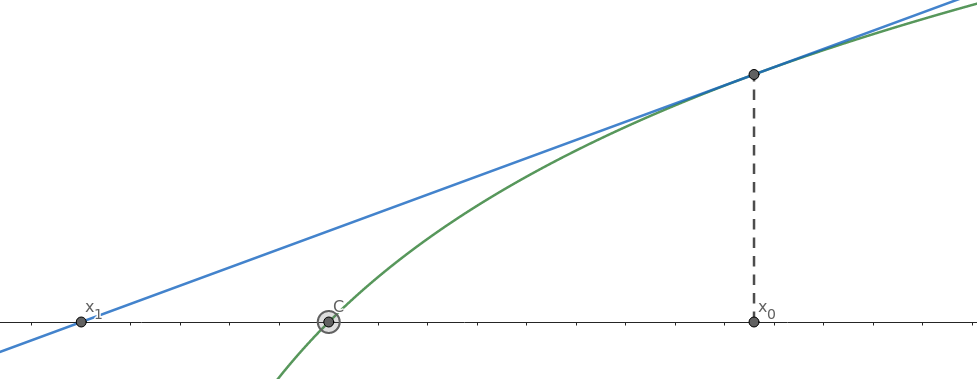
\includegraphics[scale=0.44]{../images/Newton_method.png}
\end{center}

Но самое главное здесь - это оценка.
\begin{proof}
Уравнение касательной имеет вид
\begin{equation*}
y = f(x_0) + f'(x_0)(x-x_0)
\end{equation*}
Теперь надо узнать, при каком $x_1$ $y = 0$:
\begin{align*}
(x_1 - x_0) &= -\frac{f(x_0)} {f'(x_0)}\\
x_1 &= x_0 - \frac{f(x_0)}{f'(x_0)}
\end{align*}
Теперь запускаем этот процесс рекурсивно:
\begin{equation*}
x_{n+1} = x_n - \frac{f(x_n)} {f'(x_n)}
\end{equation*}
Посмотрим, насколько быстро мы приближаемся к корню:
\begin{equation*}
C - x_{n+1} = C - x_n + \frac{f(x_n)} {f'(x_n)} = \frac{f(x_n) + f'(x_n)(C - x_n)} {f'(x_n)}
\end{equation*}
Формула Тейлора в $x_n$
\begin{equation*}
f(x) = f(x_n) + f'(x_n)(x - x_n) + \frac{f''(t_n)} {2!} (x - x^n)^2
\end{equation*}
При $x:= C$ $f(x) = 0$, первые два слагаемых равны числителю предыдущей формулы. Значит, мы можем ее продолжить:
\begin{equation*}
\frac{f(x_n) + f'(x_n)(C - x_n)} {f'(x_n)} = \frac{-\frac{1} {2} f''(t_n)(C - x_n)^2}{f'(x_n)}
\end{equation*}
Возьмем $M:= max|f''|; m:= min|f'| >0$. Тогда
\begin{equation*}
|C - x_{n+1}| \leq \frac{1} {2} \frac{|f''(t_n)||C -x_n|^2} {f'(x_n)} \leq \frac{M} {2m} |C - x_n|^2
\end{equation*}
\begin{align*}
|C - x_{n+1}| \leq \frac{M} {2m} |C - x_n|^2 \leq \frac{M}{2m}\left|\frac{M}{2m}|C - x_{n-1}|^2\right|^2 &=\\
= \left(\frac{M}{2m}\right)^{1 + 2} |C - x_{n-1}|^4 \leq \ldots &\leq \left(\frac{M}{2m}\right)^{1 + 2 + \ldots + 2^n} |C - x_1|^{2^n} = \frac{2m} {M} \left(\left(\frac{M}{2m}\right)^2|C - x_1|\right)^{2^n}
\end{align*}
Потребуем выбрать начальное приближение так, чтобы скобка была $<1$. Тогда  разница будет убывать ОЧЕНЬ быстро.
\end{proof}

\subsubsection{Иррациональность числа $e^2$ \texorpdfstring{$^3$}{}}
\textit{Формулировка: }
$e^2$ --- иррационально.
\begin{proof}
От противного. Пусть $e^2 = \frac{2k} {n} \Leftrightarrow ne = 2k\cdot e^{-1}$. Домножим все на $(2k-1)!$:
\begin{equation*}
n(2k-1)!e = (2k)!\cdot e^{-1}
\end{equation*}
Докажем, что левая часть чуть больше некоторого целого числа, а правая часть чуть меньше некоторого целого числа.

Вспомним формулу Тейлора с остатком в форме Лагранжа:
\begin{equation*}
e^x = 1 + x + \frac{x^2} {2!} + \dots + \frac{x^m} {m!} + \frac{e^c} {(m+1)!} x^{m+1} \qquad c \in (0, x)
\end{equation*}
Теперь будем подставлять в эту формулу $x = 1$ и $x = -1$:
\begin{equation*}
n(2k-1)!e = n(2k-1)!\left(1 + 1 + \frac{1} {2!} + \dots + \frac{1} {(2k - 1)!}\right) + n(2k-1)!\frac{e^c} {(2k)!}\qquad c \in (0, 1)
\end{equation*}
Заметим, что левое слагаемое --- целое число. Оценим остаток:
\begin{equation*}
n(2k-1)!\frac{e^c} {(2k)!} = \frac{n}{2k}e^c = e^{c-2} < e^{-1} < \frac{1} {2}
\end{equation*}
\begin{equation*}
(2k)!\cdot e^{-1} = (2k)!\left(1 -1 + \frac{1} {2!} +  \dots + \frac{1} {(2k)!}\right) - \frac{e^c} {(2k + 1)!} \qquad c \in (-1, 0)
\end{equation*}
Левое слагаемое, кстати, тоже целое число. $e^2 = \frac{2k} {n}$, тогда, очевидно, $k>1$. Оцениваем остаток:
\begin{equation*}
\frac{e^c} {(2k + 1)!} < \frac{1} {2k + 1} < \frac{1} {3}
\end{equation*}
Итого, есть целое число, от которого мы смещаемся вправо меньше, чем на $\frac{1} {2}$ и целое число, от которого мы смещаемся влево меньше, чем на $\frac{1} {3}$ и приходим в одно и то же число. Абсурд.
\end{proof}

\subsubsection{Теорема Брауэра\texorpdfstring{$^3$}{}}

\textit{Формулировка:}
\begin{enumerate}
\item $F: B(0, 1) \subset \mathbb{R}^m \rightarrow B(0, 1) \subset \mathbb{R}^m \text{ непрерывно, тогда } \exists x \in B(0, 1): F(x) = x$
\item $F: [0, 1]^m \rightarrow [0, 1]^m - \text{ непрерывно, тогда } \exists x \in [0, 1]^m F(x) = x$
\end{enumerate}

Более подробно про теорему Брауэра и игру Гекс можно посмотреть тут \href{https://arxiv.org/abs/1409.7890}{тык}

\paragraph{Игра Гекс}
Поле для игры состоит из "прямоугольника", составленного из правильных шестиугольников (см. рисунок). Две противоположные стороны назовем черными, две другиие --- белыми. Игроки ходят по очереди, крася один из шестиугольников в черный или белый цвет, их цель --- проложить дорожку либо от черной стороны к черной, либо от белой к белой. Проложивший дорожку, выигрывает.
\begin{center}
    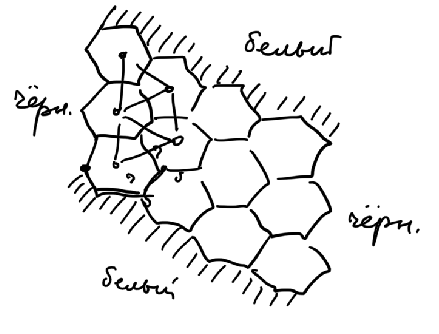
\includegraphics[scale=0.44]{../images/Brauer's_th.png}
\end{center}

\textit{Лемма.}

\textit{Формулировка:}

Любая раскраска для игры Гекс будет выигрышна для одной из сторон

\begin{proof}
Накидаем случайную раскраску шестигранников в черный и белый цвета. Рассмотрим точку на "левом нижнем" шестиграннике, которая будет одновременно и на белой и на черной стороне (на рисунке выше --- толстая черная точка). Начнем обходить шестиграннике по следующему правилу: черные шестигранники оставляем по левой руке, белые --- по правой. Теперь думаем, к чему это нас может привести: мы не можем зайти в цикл, не касающийся сторон из-за выбранного правила обхода. Тогда, т.к. всего конечное число гексов, мы рано или поздно выйдем на границу. Но начинали мы с точки, которая принадлежит и белой, и черной стороне. Значит, мы победили.
\end{proof}

Теперь вместо Гексов будем рассматривать граф, вершинами которого являются гексы, а ребрами --- наличие соприкосновения между ними. Пусть он имеет размер $n \times n$.
Каждому узлу $(k, l)$ будем сопоставлять точку $\left(\frac{k}{n}, \frac{l}{n}\right)$. По только что доказанной лемме существует ломаная из одной стороны в противоположную по узлам одного цвета.

\begin{center}
    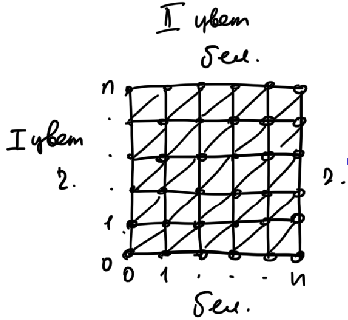
\includegraphics[scale=0.44]{../images/Brauer's_th2.png}
\end{center}

\paragraph{Доказательство теоремы Брауэра}
\begin{proof}
$F:[0, 1]^2 \rightarrow [0, 1]^2$, $x = (x_1, x_2)$, $F(x) = \left(f_1(x), f_2(x)\right)$
Введем необходимые обозначения:
$x, y \in \mathbb{R}^2$, $\| x, y\|$ - расстояние, $\rho(x, y) = max(|x_1 - y_1|, |x_2 - y_2|)$ --- непрерывна в $\mathbb{R}^2 \times \mathbb{R}^2$
Функция $x \in [0, 1]^2 \rightarrow \rho\left(x, F(x)\right)$ --- непрерывна на $[0, 1]^2$

Вот только теперь начинается доказательство. Доказывать будем от противного: пусть $\forall x: F(x) \neq x$.
По теореме Вейерштрасса:
\begin{equation}\label{Vey_th}
\exists \varepsilon > 0 \forall x \in [0, 1]^2 \rho\left(x, F(x)\right) \geq \varepsilon
\end{equation}
По теореме Кантора (для $F$, и $x = [0, 1]^2$) $F$ --- равномерно непрерывна на $[0, 1]^2$, т.е. для этого $\varepsilon \exists \delta > 0$ (НУО $\delta \leq \varepsilon$) $\forall x, \bar{x} \|x - \bar{x} \| < \delta \|F(x) - F(\bar{x})\| < \varepsilon$.

Возьмем $\frac{\sqrt{2}}{n} < \delta$, построим доску $HEX(n, n)$ и начнем ее красить. Но красить будем не от балды. $v = (v_1, v_2), v_1, v_2 \in \mathbb{Z}_+$ --- узел доски $HEX(n, n)$. 
\begin{equation}
color(V) = min\left\{i\in\{1, 2\}: \left| f_i\left(\frac{v} {n}\right) - \frac{v_i} {n}\right| \geq \varepsilon\right\}\notag
\end{equation}
это определение корректно в силу \eqref{Vey_th}.
По лемме об игре в Гекс существет ломаная $I$ цвета от одной вертикальной стороны квадрата к другой, либо ломаная $II$ цвета от одной горизонтальной стороны квадрата к другой.

\begin{center}
    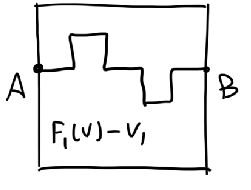
\includegraphics[scale=0.44]{../images/Brauer's_th3.png}
\end{center}

$f_i - i$-тая координата $F$.

В т.A: $f_i(A) \geq 0, A_1 = 0 \Rightarrow f_1(A) - A_1 \geq \varepsilon$

В т.B: $f_i(B) \leq 1, B_1 = 1 \Rightarrow f_1(B) - B \leq - \varepsilon$

То есть, в какой-то момент, мы совершили скачок на $\geq 2\varepsilon$, но при переходе от одного узла к другому каждая координата меняется на $\frac{1} {n} < \delta \leq \varepsilon$, т.е. сумма меняется $ < 2\varepsilon$.
В случае, когда мы двигаемся по диагонали, мы рассматриваем то же $\delta$, и проводим аналогичные рассуждения.

Противоречие.

\end{proof}

\end{document}
